\documentclass{beamer}
\usepackage{beamerthemeCVC}
\usepackage{graphicx}

\usepackage{xmpmulti}

%% PRESENTATION CONFIGURATION PARAMETERS %%%%%%%%%%%%%%%%%%%%%%%%%%%%%%%%%%%%%%%
\titlebackgroundfile{images/template_title}
%\framebackgroundfile{images/template_frame}
\framebackgroundfile{images/template_frame_v01}
%\definecolor{vermell}{HTML}{8C2423}
\definecolor{vermell}{HTML}{000066}
\definecolor{gris}{HTML}{4C4C4C}

\usefonttheme{structurebold}

\setbeamercolor{author in head/foot}{fg=white}
\setbeamercolor{title in head/foot}{fg=white}
\setbeamercolor{section in head/foot}{fg=vermell}
\setbeamercolor{normal text}{fg=gris}
\setbeamercolor{frametitle}{fg=vermell}
%\setbeamercolor{frametitle}{fg=blue!20!black}
\setbeamerfont{block title}{size={}}
\setbeamerfont{author}{size=\footnotesize}
\setbeamerfont{date}{size=\footnotesize}
\setbeamertemplate{itemize item}[circle]
\setbeamertemplate{itemize subitem}[circle]
\setbeamertemplate{itemize subsubitem}[circle]
\setbeamertemplate{itemize subsubsubitem}[circle]
\setbeamercolor{itemize item}{fg=vermell}
\setbeamercolor{itemize subitem}{fg=vermell}
\setbeamercolor{itemize subsubitem}{fg=vermell}
\setbeamercolor{itemize subsubsubitem}{fg=vermell}
\setbeamercolor{enumerate item}{fg=vermell}
\setbeamercolor{enumerate subitem}{fg=vermell}
\setbeamercolor{enumerate subsubitem}{fg=vermell}
\setbeamercolor{enumerate subsubsubitem}{fg=vermell}
\setbeamercolor{alerted text}{fg=vermell}
\setbeamerfont{alerted text}{series=\bfseries}
% This command makes that acrobat reader doesn't changes the colors of the slide
% when there are figures with transparencies.
\pdfpageattr {/Group << /S /Transparency /I true /CS /DeviceRGB>>}




\graphicspath{{images/}}



%%%%%%%%%%%%%%%%%%%%%%%%%%%%%%%%%%%%%%%%%%%%%%%%%%%%%%%%%%%%%%%%%%%%%%%%%%%%%%%%

%      + Short title.               + Title which appears in the cover.
%      v                            v
%\title[Beamer presentation example]{Nonlinear Dynamics Approach to Human Activity Recognition Using Inertial Sensors}
\vspace{5mm}
\title[Quantifying Dexterity in Human Activities ̣Through the Time-delay Embedded  Phase Space Representation]
{Quantifying Dexterity in Human Activities ̣\\ Through the Time-delay Embedded \\ Phase Space Representation}
%       + Short author names which appear in the slides.
%       v
\author[Miguel Perez-Xochicale]
{   % Author names which appear in the cover page.
    %Perez-Xochicale Miguel Angel\inst{1}
    \textbf{Miguel Perez-Xochicale}
}
%          + Short affiliation which appears in the slides.
%          v
\institute[CVC-IIIA]
{   % Affiliation information which appears in the cover page.

      \vspace{5mm}
    \begin{tabular}{c}
    %\inst{1}Internal Research Conference 
    \end{tabular}
}
%     + Short acronym of the conference or date of the presentation.
%     v
\date[DEMO-2013]
{   % Conference name which appears in the cover page.
     18th May 2015
}





\begin{document}
% Creates the cover page.
\frame{\titlepage}





%+++++++++++++++++++++++++++++++++++++++++++++++++++
%+++++++++++++++++++++++++++++++++++++++++++++++++++
\section{Literature Review}


%%%%%%%%%%%%%%%%%%
%%%%%%%%%%%%%%%%%%
%SECTION00






% 
% %+++++++++++++++++++++++++++++++++++++++++++++++++++
% \begin{frame}
% 	\frametitle{Why is HAR a challenging task?}
% \vspace{-0.5cm}
% \begin{figure}
%  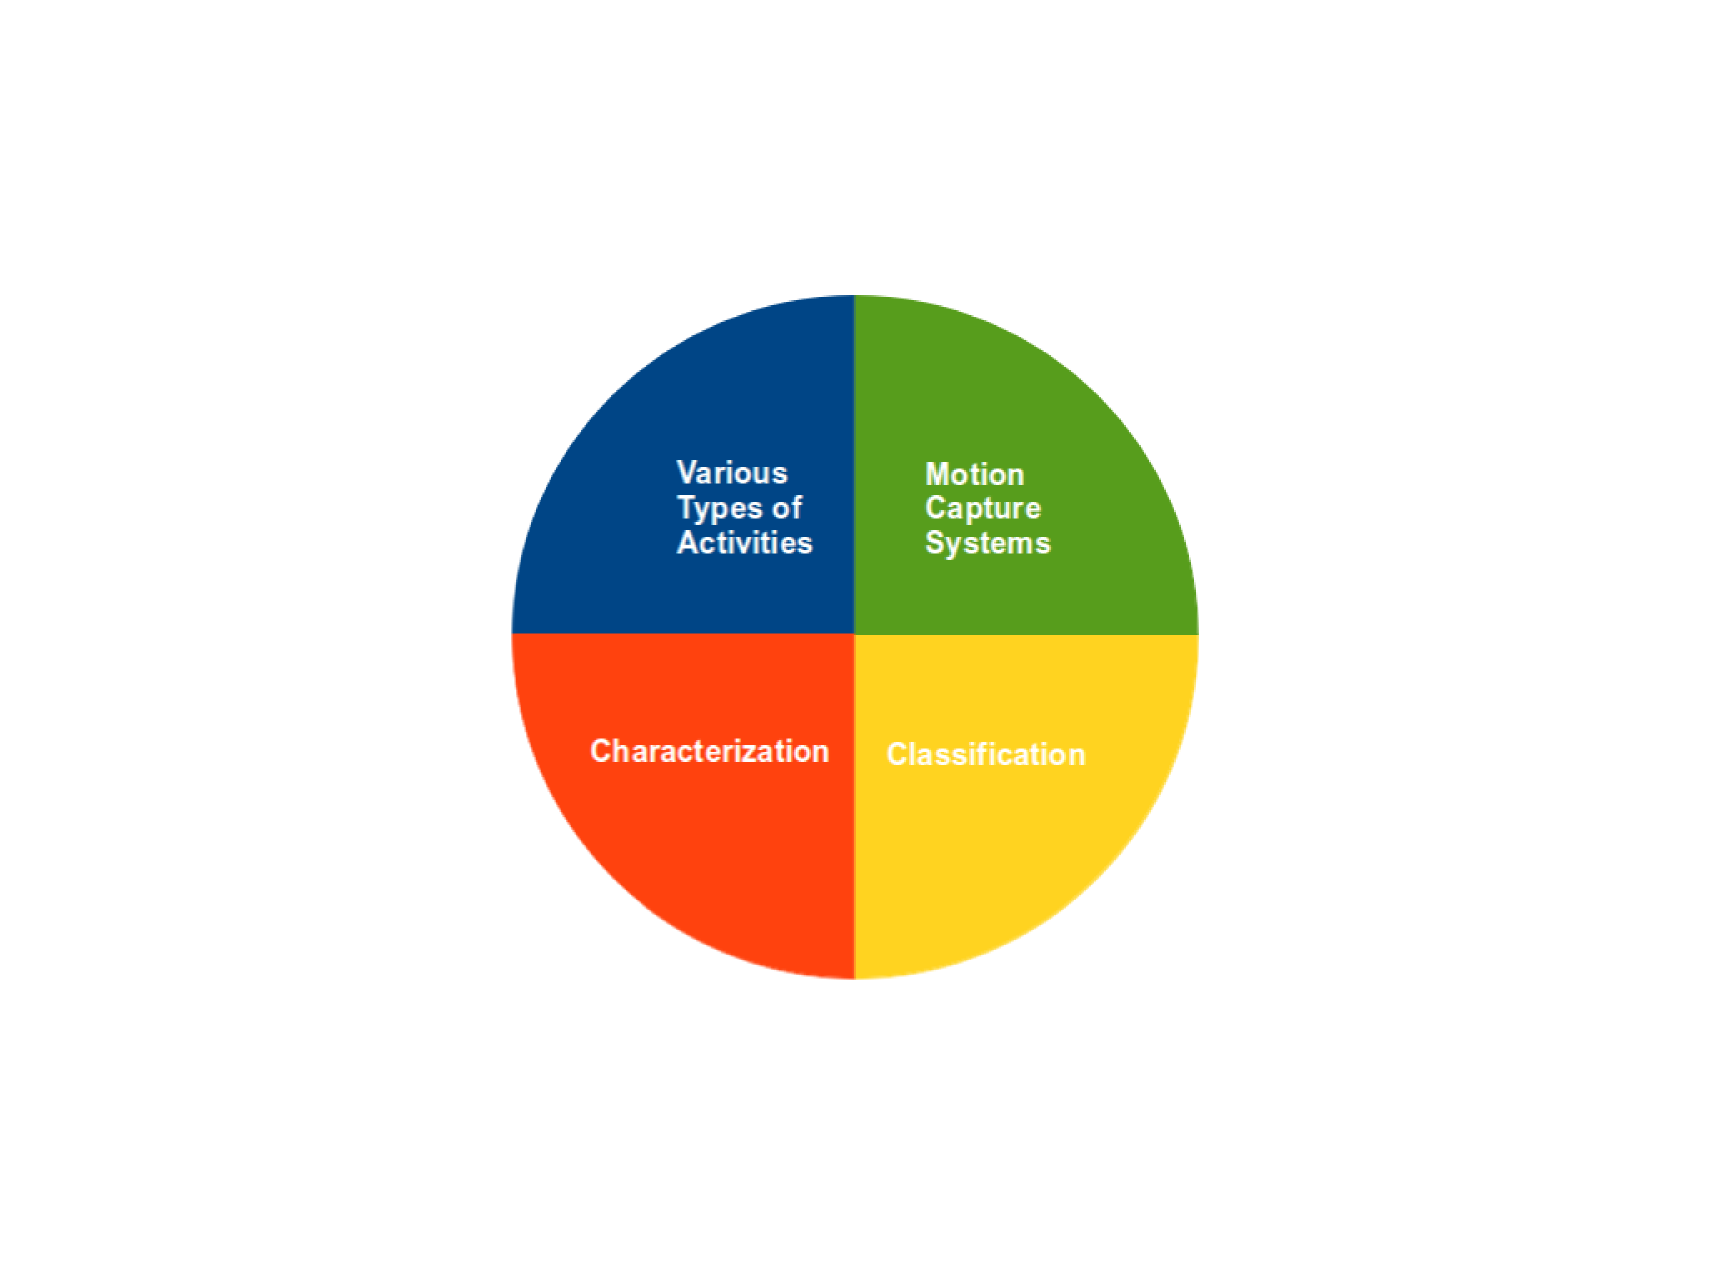
\includegraphics[scale=.3]{har00}
% \vspace{-0.6cm}
% %  \caption{Reconstructed State Space Via Taken's Theorem}
% \end{figure}
% \end{frame}
% %---------------------------------------------------
% 
% %+++++++++++++++++++++++++++++++++++++++++++++++++++
% \begin{frame}
% 	\frametitle{Why is HAR a challenging task?}
% \vspace{-0.5cm}
% \begin{figure}
%  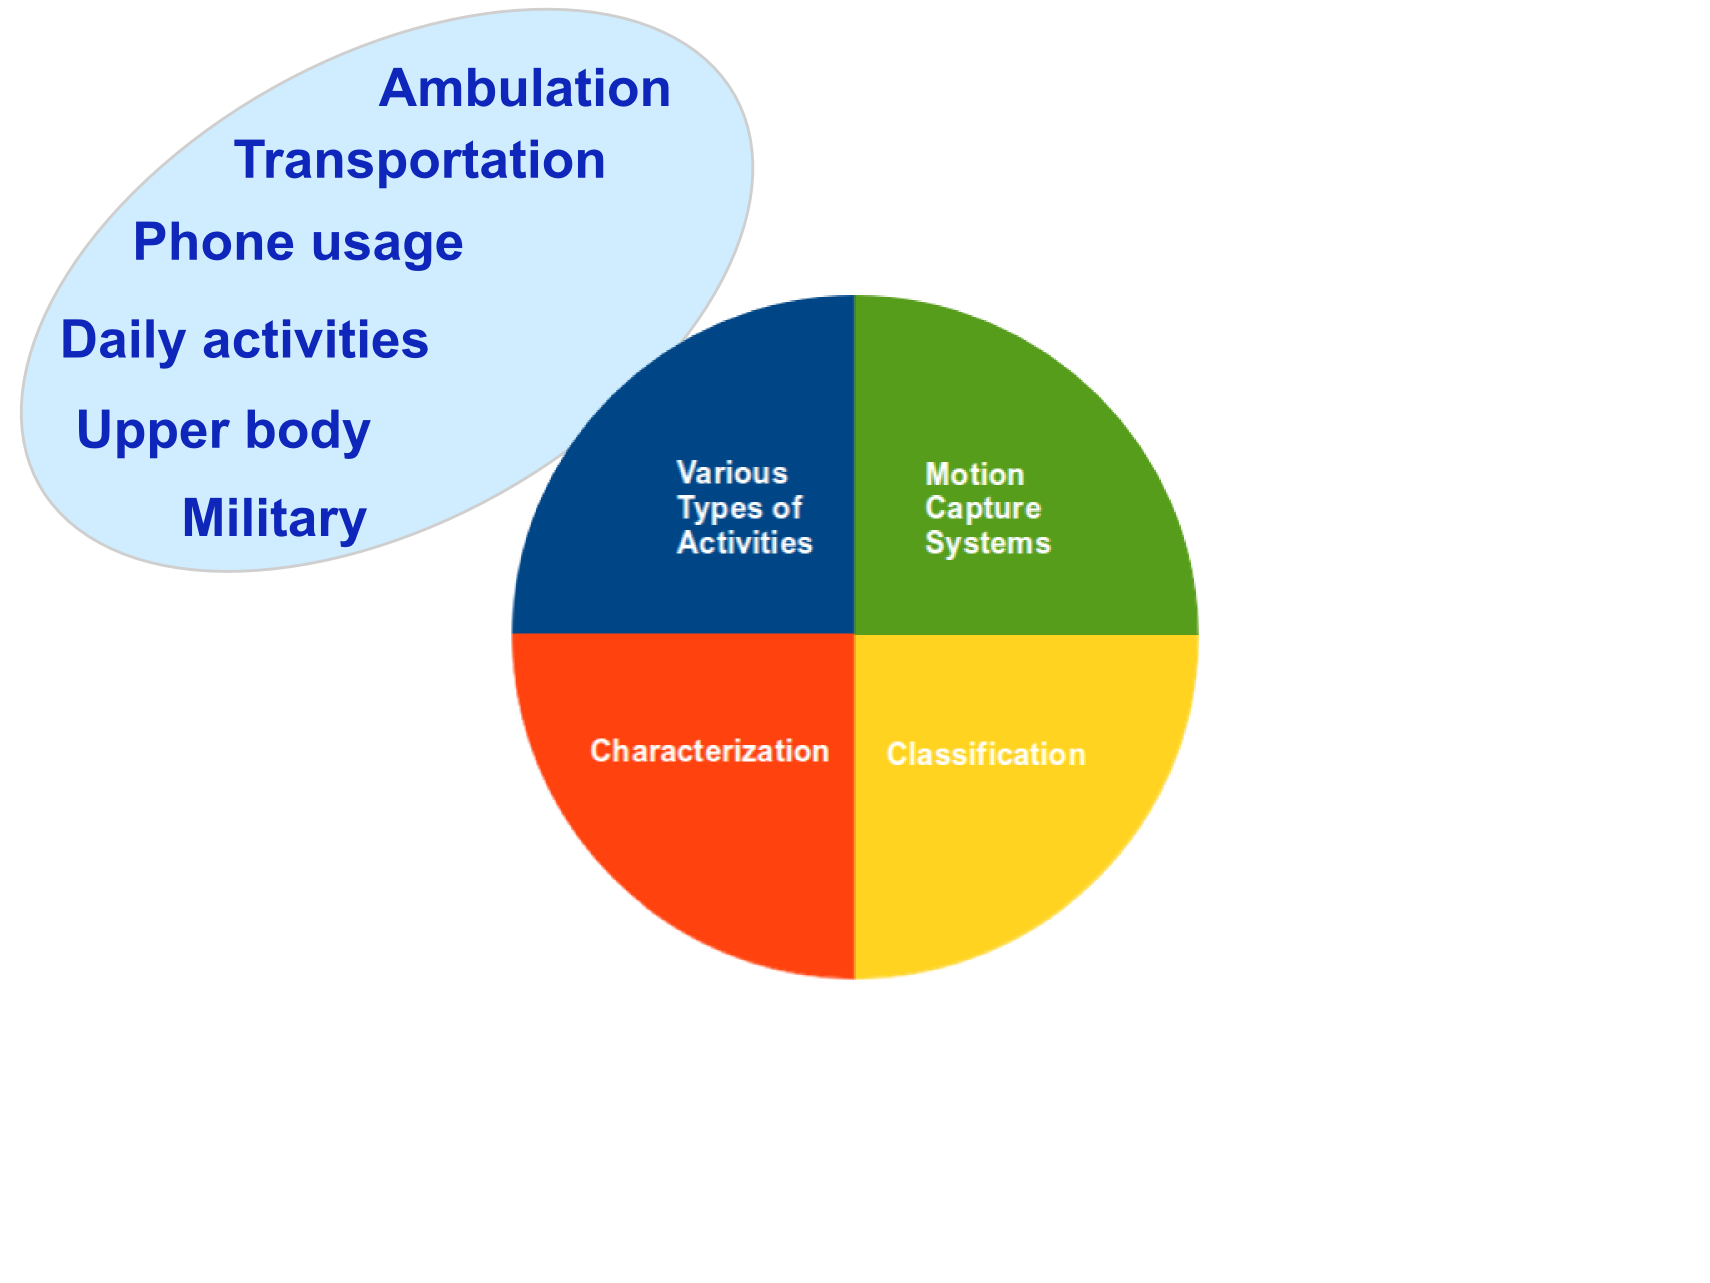
\includegraphics[scale=.3]{har02}
% \vspace{-0.6cm}
% %  \caption{Reconstructed State Space Via Taken's Theorem}
% \end{figure}
% \end{frame}
% %---------------------------------------------------
% 
% %+++++++++++++++++++++++++++++++++++++++++++++++++++
% \begin{frame}
% 	\frametitle{Why is HAR a challenging task?}
% \vspace{-0.5cm}
% \begin{figure}
%  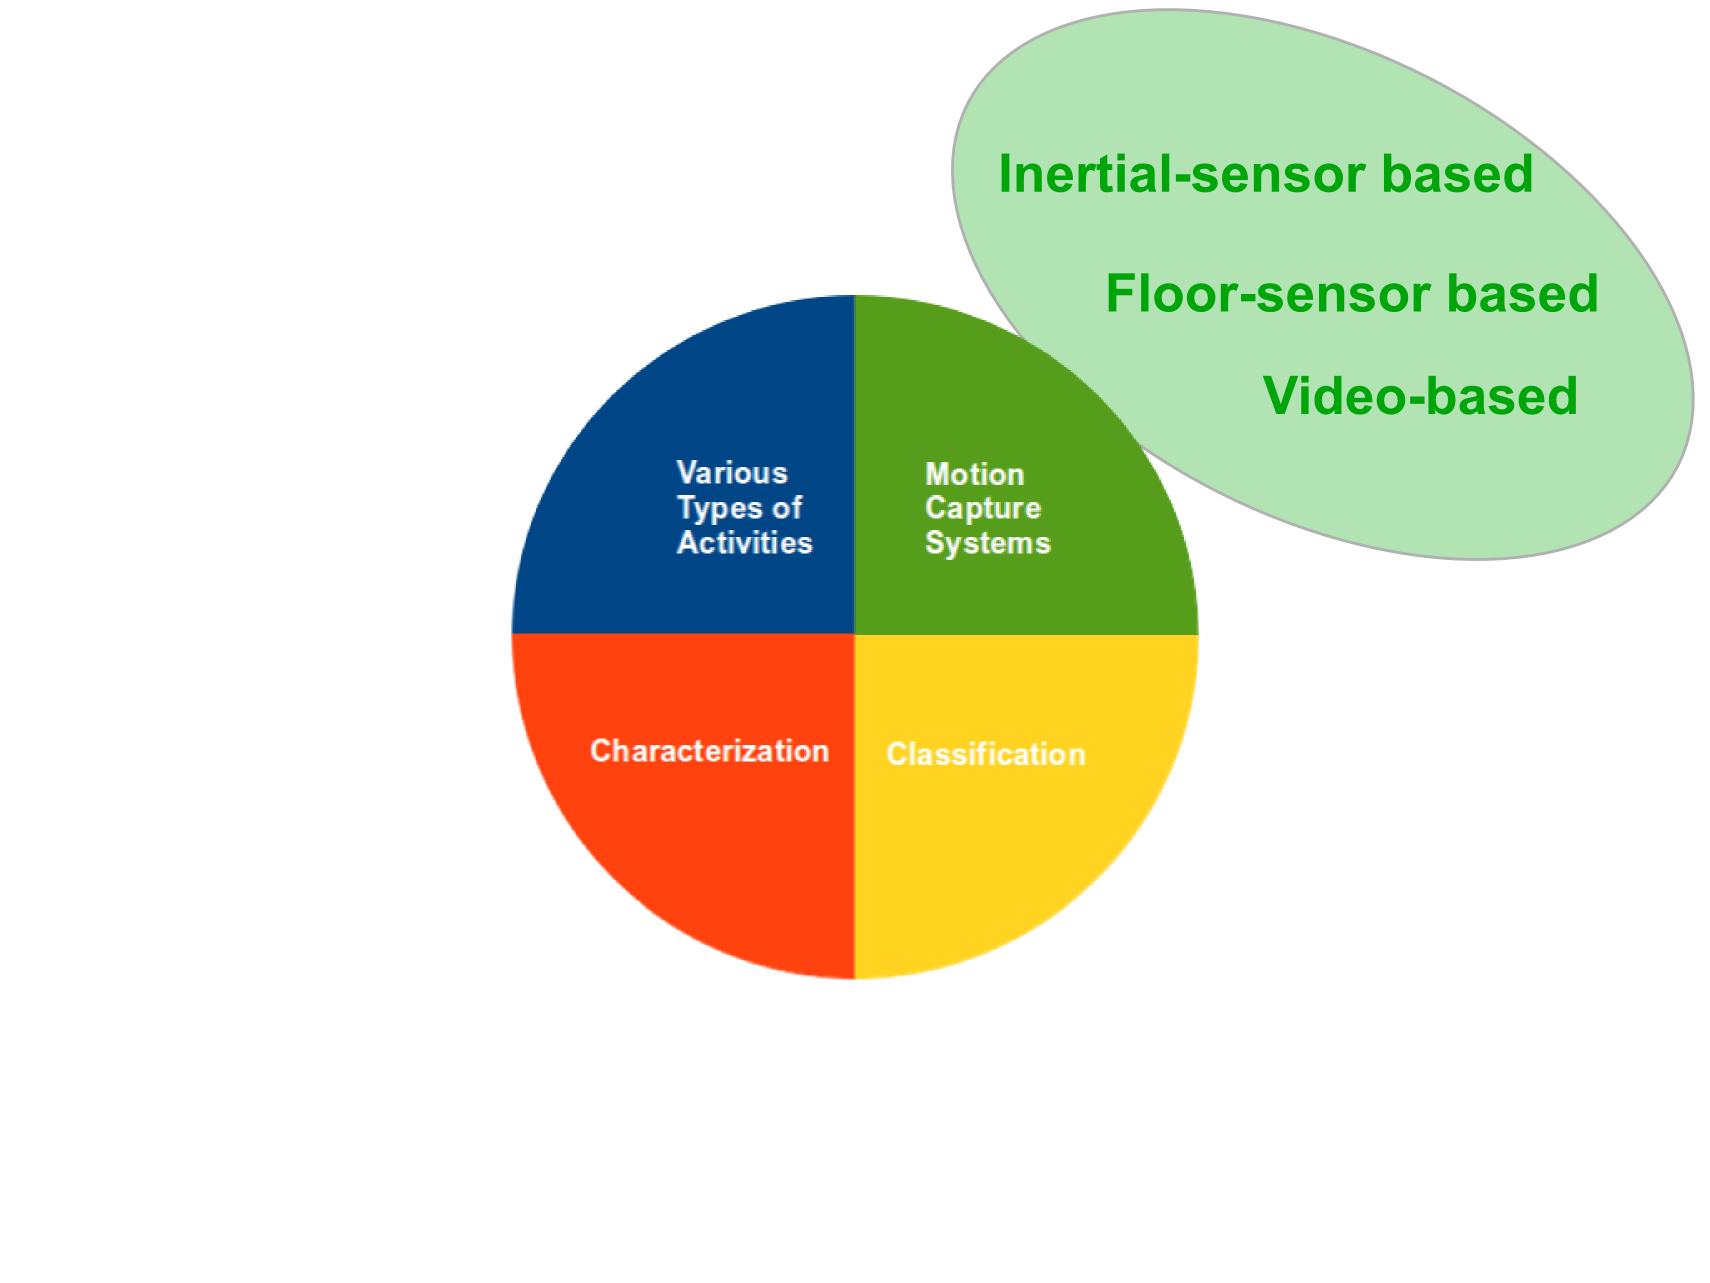
\includegraphics[scale=.3]{har03}
% \vspace{-0.6cm}
% %  \caption{Reconstructed State Space Via Taken's Theorem}
% \end{figure}
% \end{frame}
% %---------------------------------------------------
% 
% %+++++++++++++++++++++++++++++++++++++++++++++++++++
% \begin{frame}
% 	\frametitle{Why is HAR a challenging task?}
% \vspace{-0.5cm}
% \begin{figure}
%  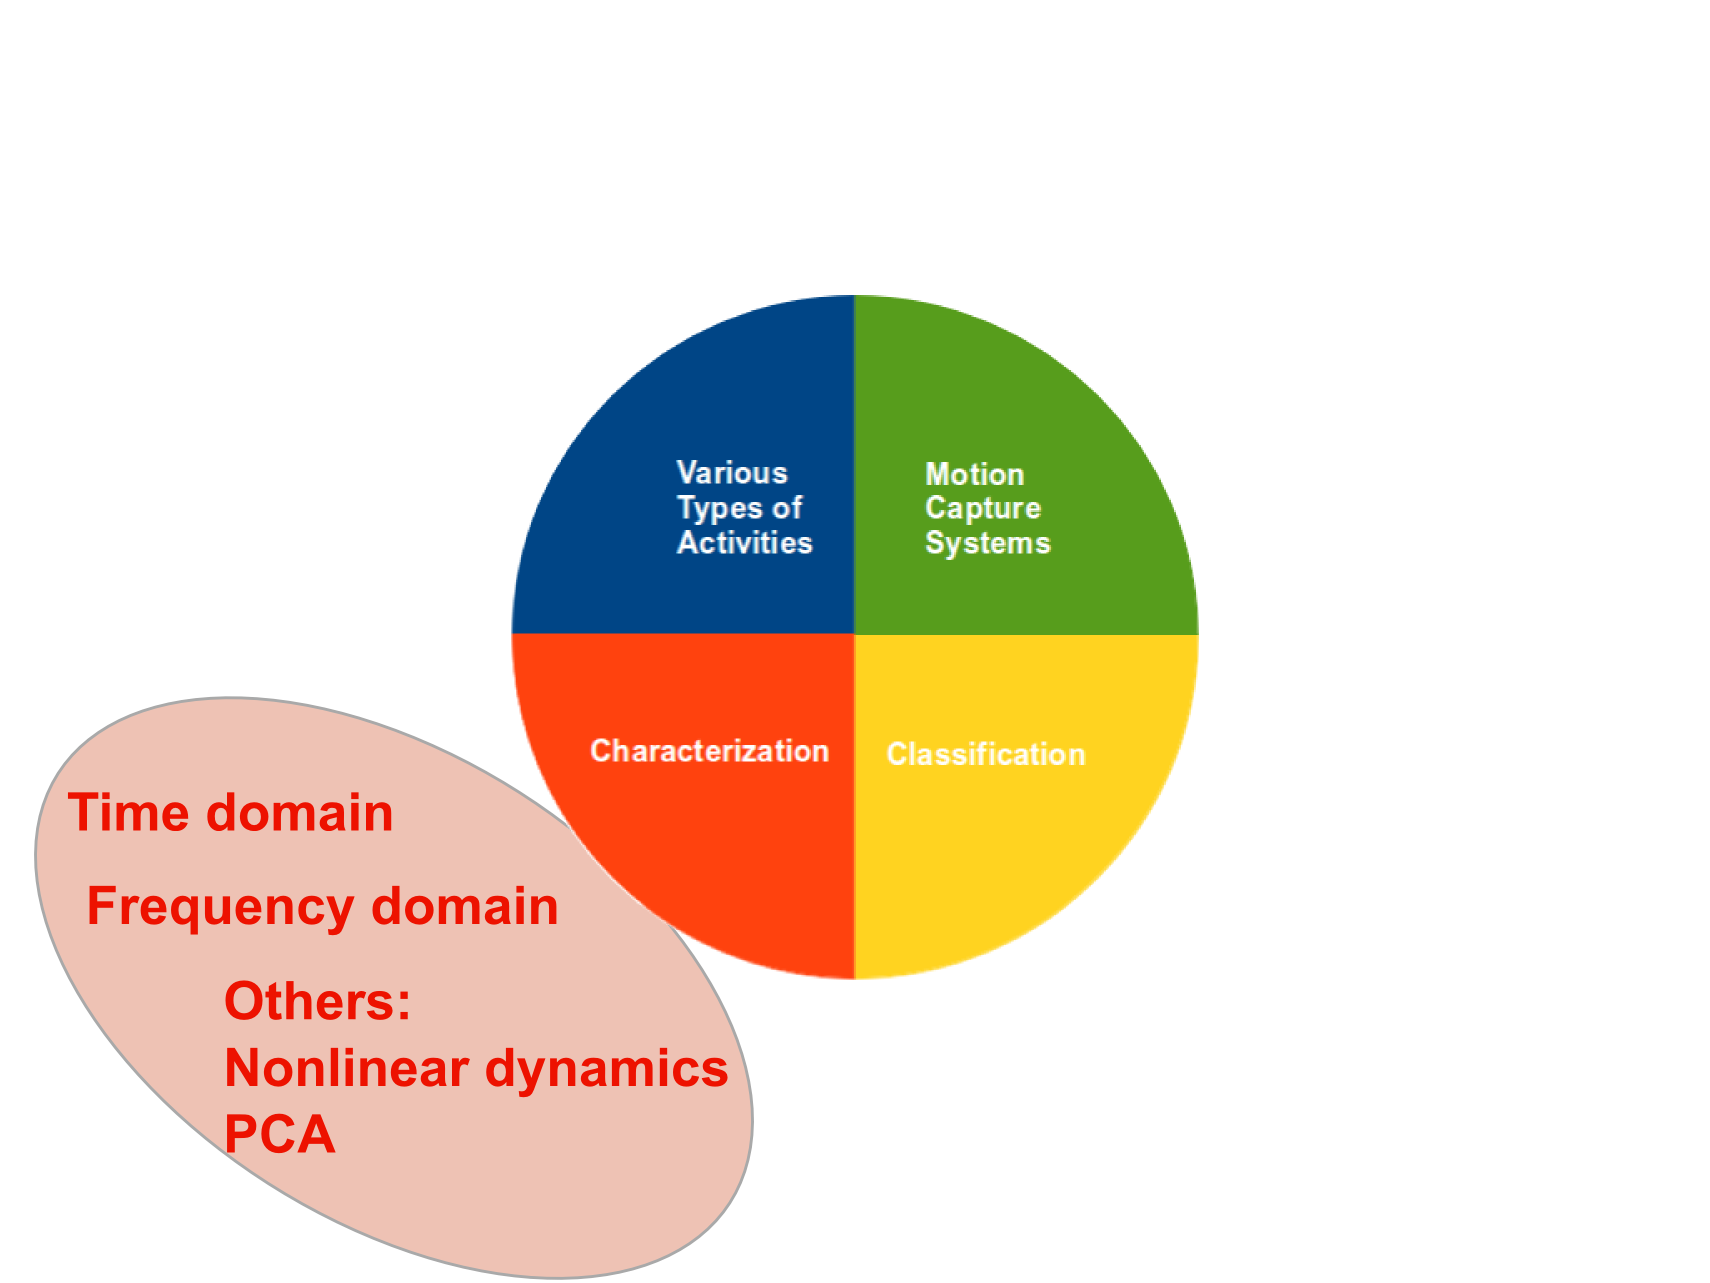
\includegraphics[scale=.3]{har05}
% \vspace{-0.6cm}
% %  \caption{Reconstructed State Space Via Taken's Theorem}
% \end{figure}
% \end{frame}
% %---------------------------------------------------
% 
% 
% %+++++++++++++++++++++++++++++++++++++++++++++++++++
% \begin{frame}
% 	\frametitle{Why is HAR a challenging task?}
% \vspace{-0.5cm}
% \begin{figure}
%  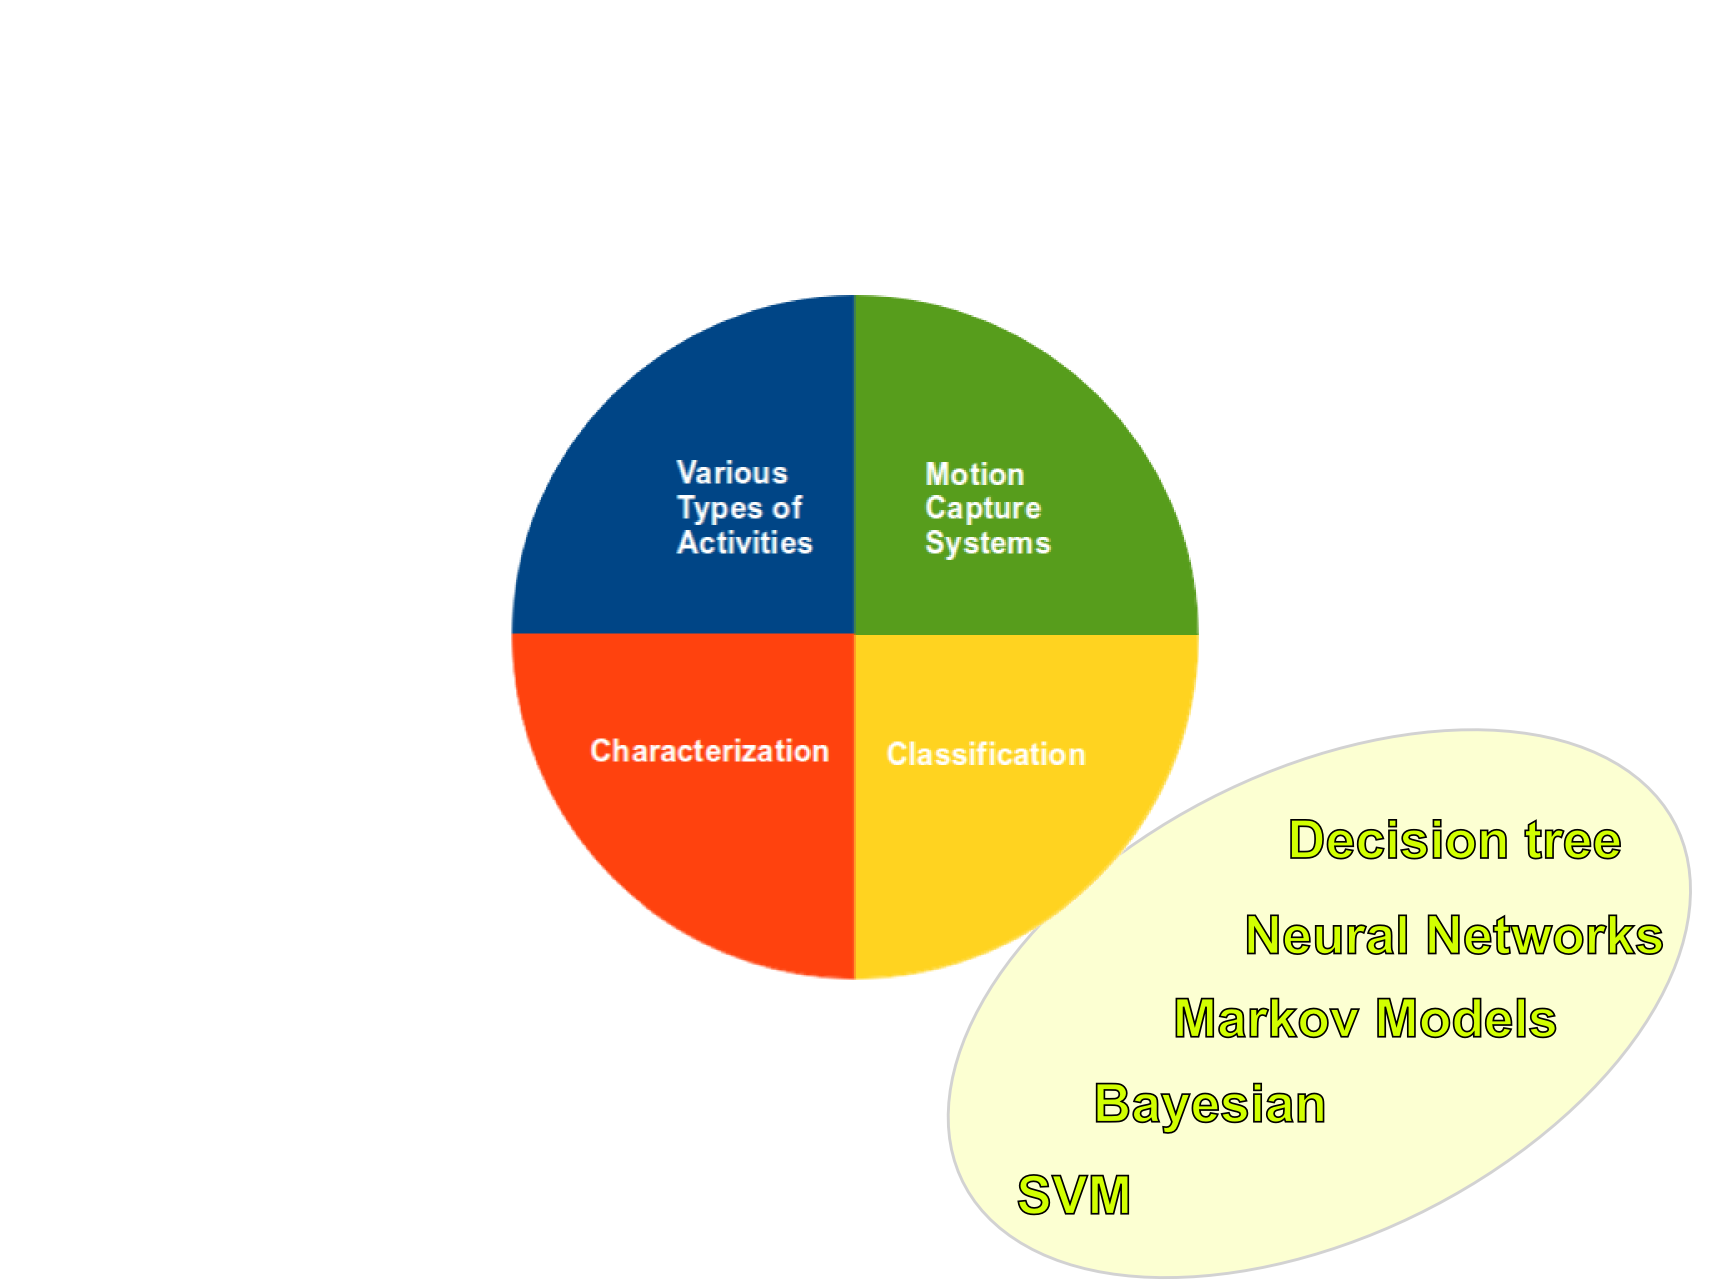
\includegraphics[scale=.3]{har04}
% \vspace{-0.6cm}
% %  \caption{Reconstructed State Space Via Taken's Theorem}
% \end{figure}
% \end{frame}
% %---------------------------------------------------



%+++++++++++++++++++++++++++++++++++++++++++++++++++
\begin{frame}
	\frametitle{Why is HAR a challenging task?}
\vspace{-0.5cm}
\begin{figure}
 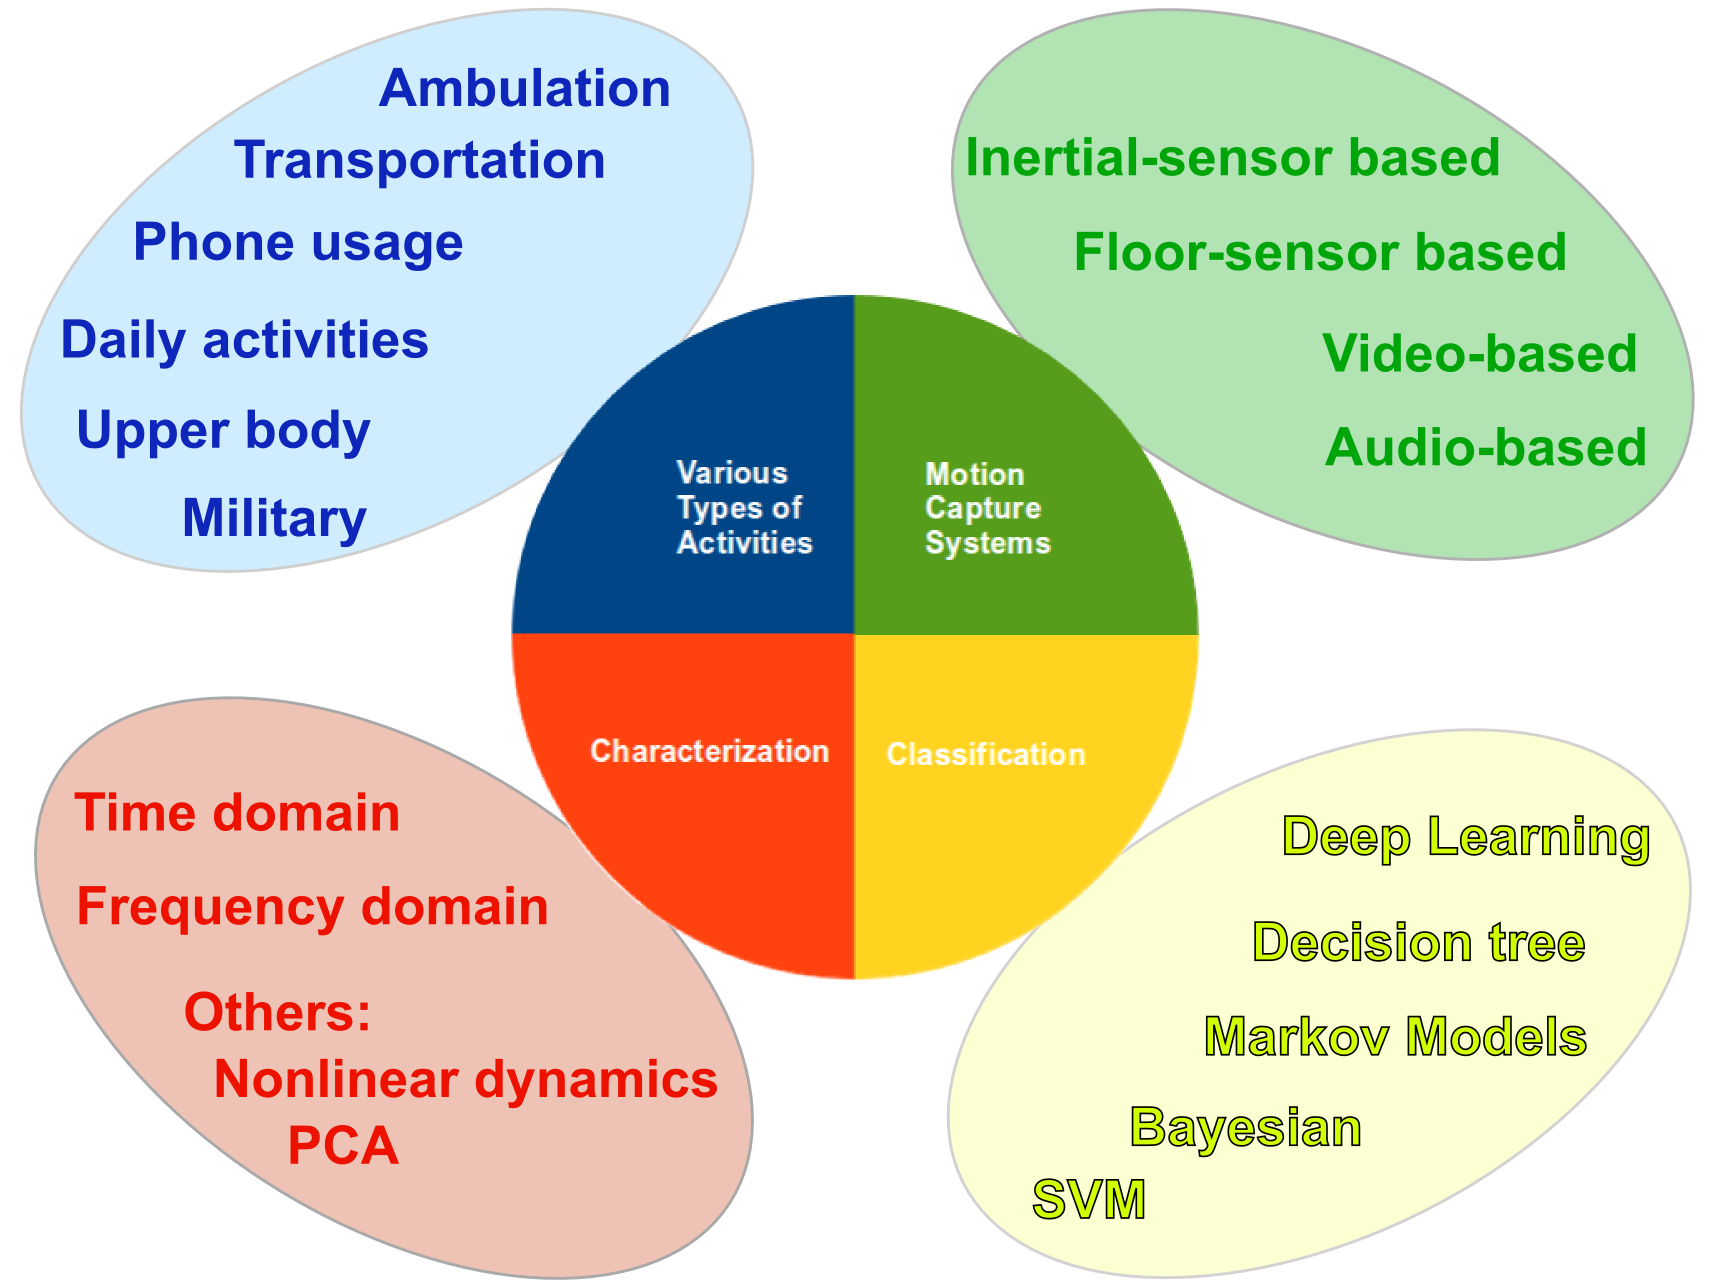
\includegraphics[scale=.3]{har_v0}
\vspace{-0.6cm}
%  \caption{Reconstructed State Space Via Taken's Theorem}
\end{figure}
\end{frame}
%---------------------------------------------------



%%%%%%%%%%%%%%%%%%
%%%%%%%%%%%%%%%%%%
%SECTION01



%+++++++++++++++++++++++++++++++++++++++++++++++++++
\begin{frame}
\frametitle{Study of electrophysiological time series}
\vspace{-0.5cm}
\begin{center}
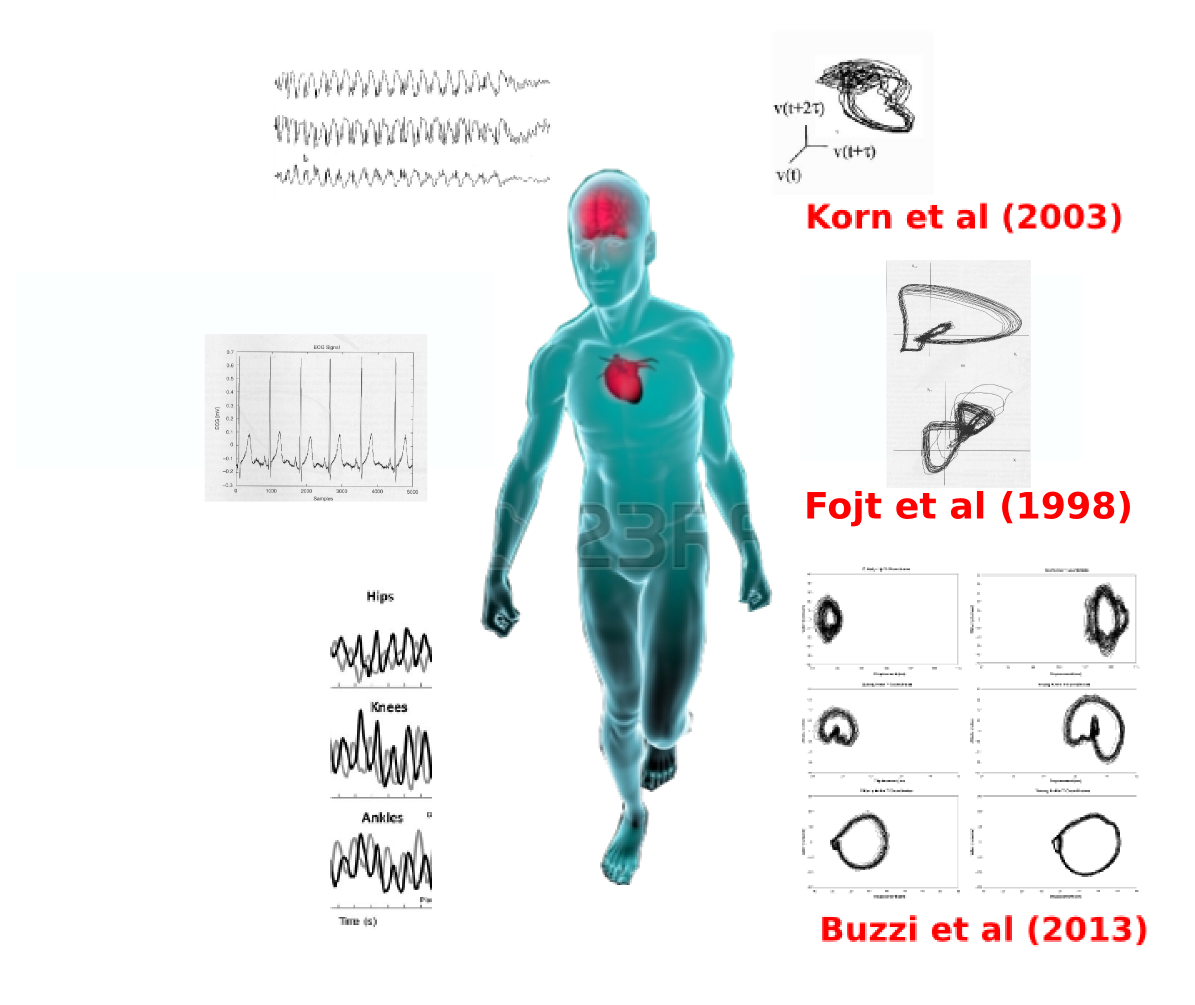
\includegraphics[scale=.4]{nonlinear_dynamics_in_humanbody_00}
\end{center}
\end{frame}
%---------------------------------------------------





%+++++++++++++++++++++++++++++++++++++++++++++++++++
\begin{frame}
\frametitle{Time Series Classification}
\vspace{-0.5cm}
\begin{center}
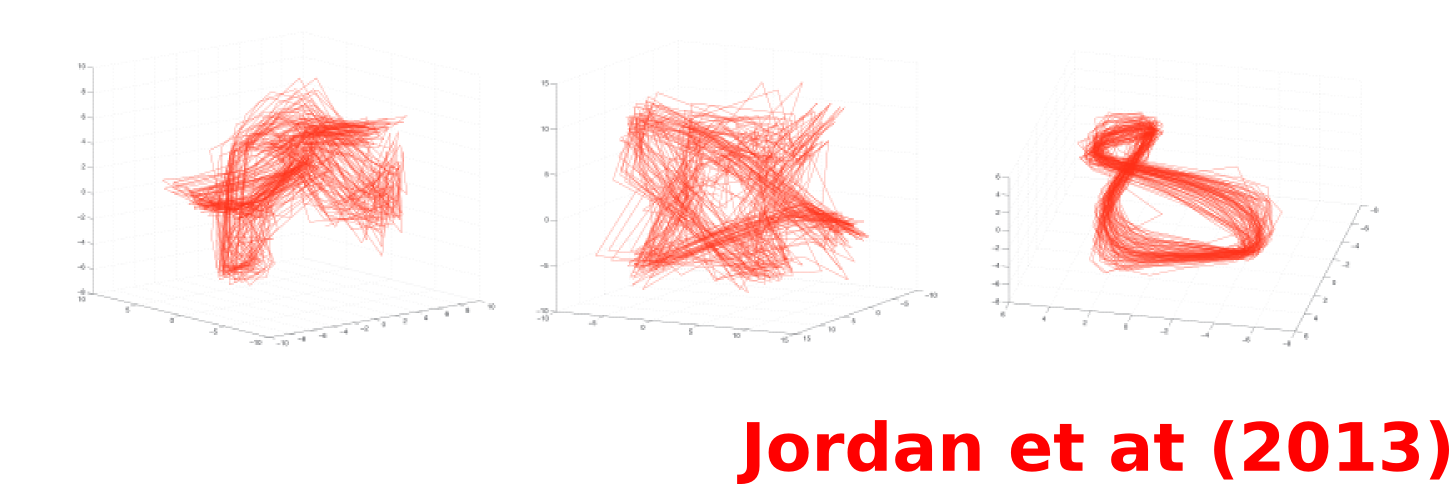
\includegraphics[scale=.45]{jordan2013}\\
Reconstructed state spaces for walking (left), running (middle), and biking (right) from
noisy accelerometer data.
\end{center}
\end{frame}
%---------------------------------------------------

%+++++++++++++++++++++++++++++++++++++++++++++++++++
\begin{frame}
\frametitle{Gait Identification}
\vspace{-0.5cm}
\begin{center}
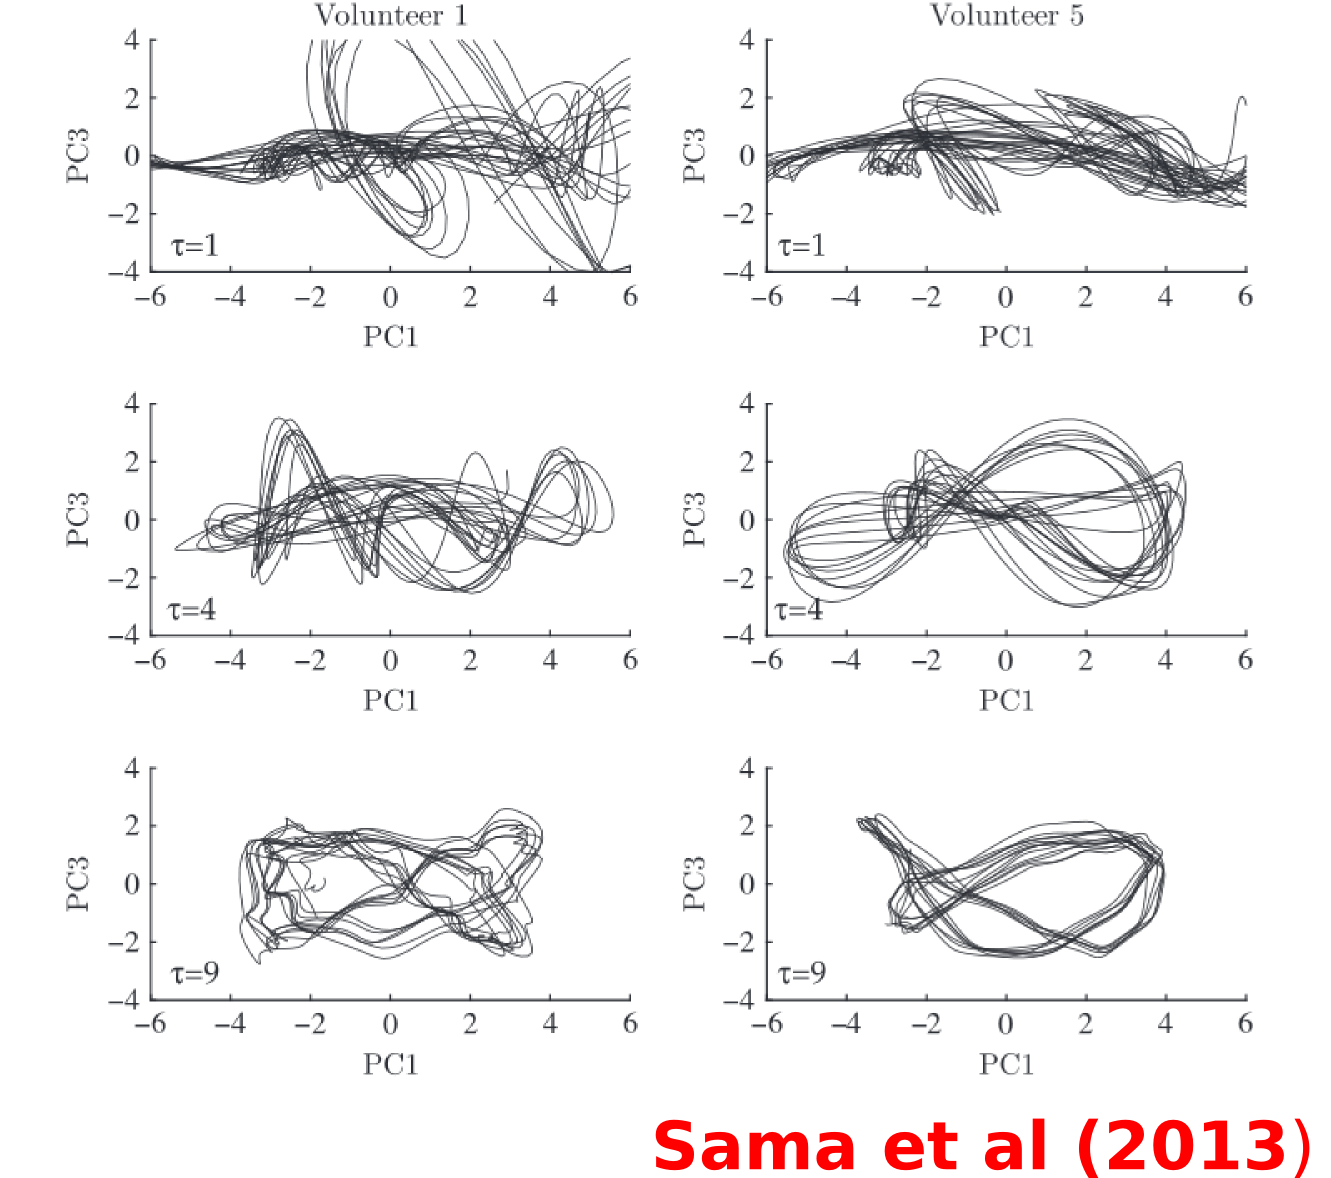
\includegraphics[scale=.3]{sama2013}\\
Reconstruction of the trajectory of the first and third PC for two indivials.
\end{center}
\end{frame}
%---------------------------------------------------



%+++++++++++++++++++++++++++++++++++++++++++++++++++
\begin{frame}
\frametitle{Dexterity of Tennis Players}
\vspace{-0.5cm}
\begin{center}
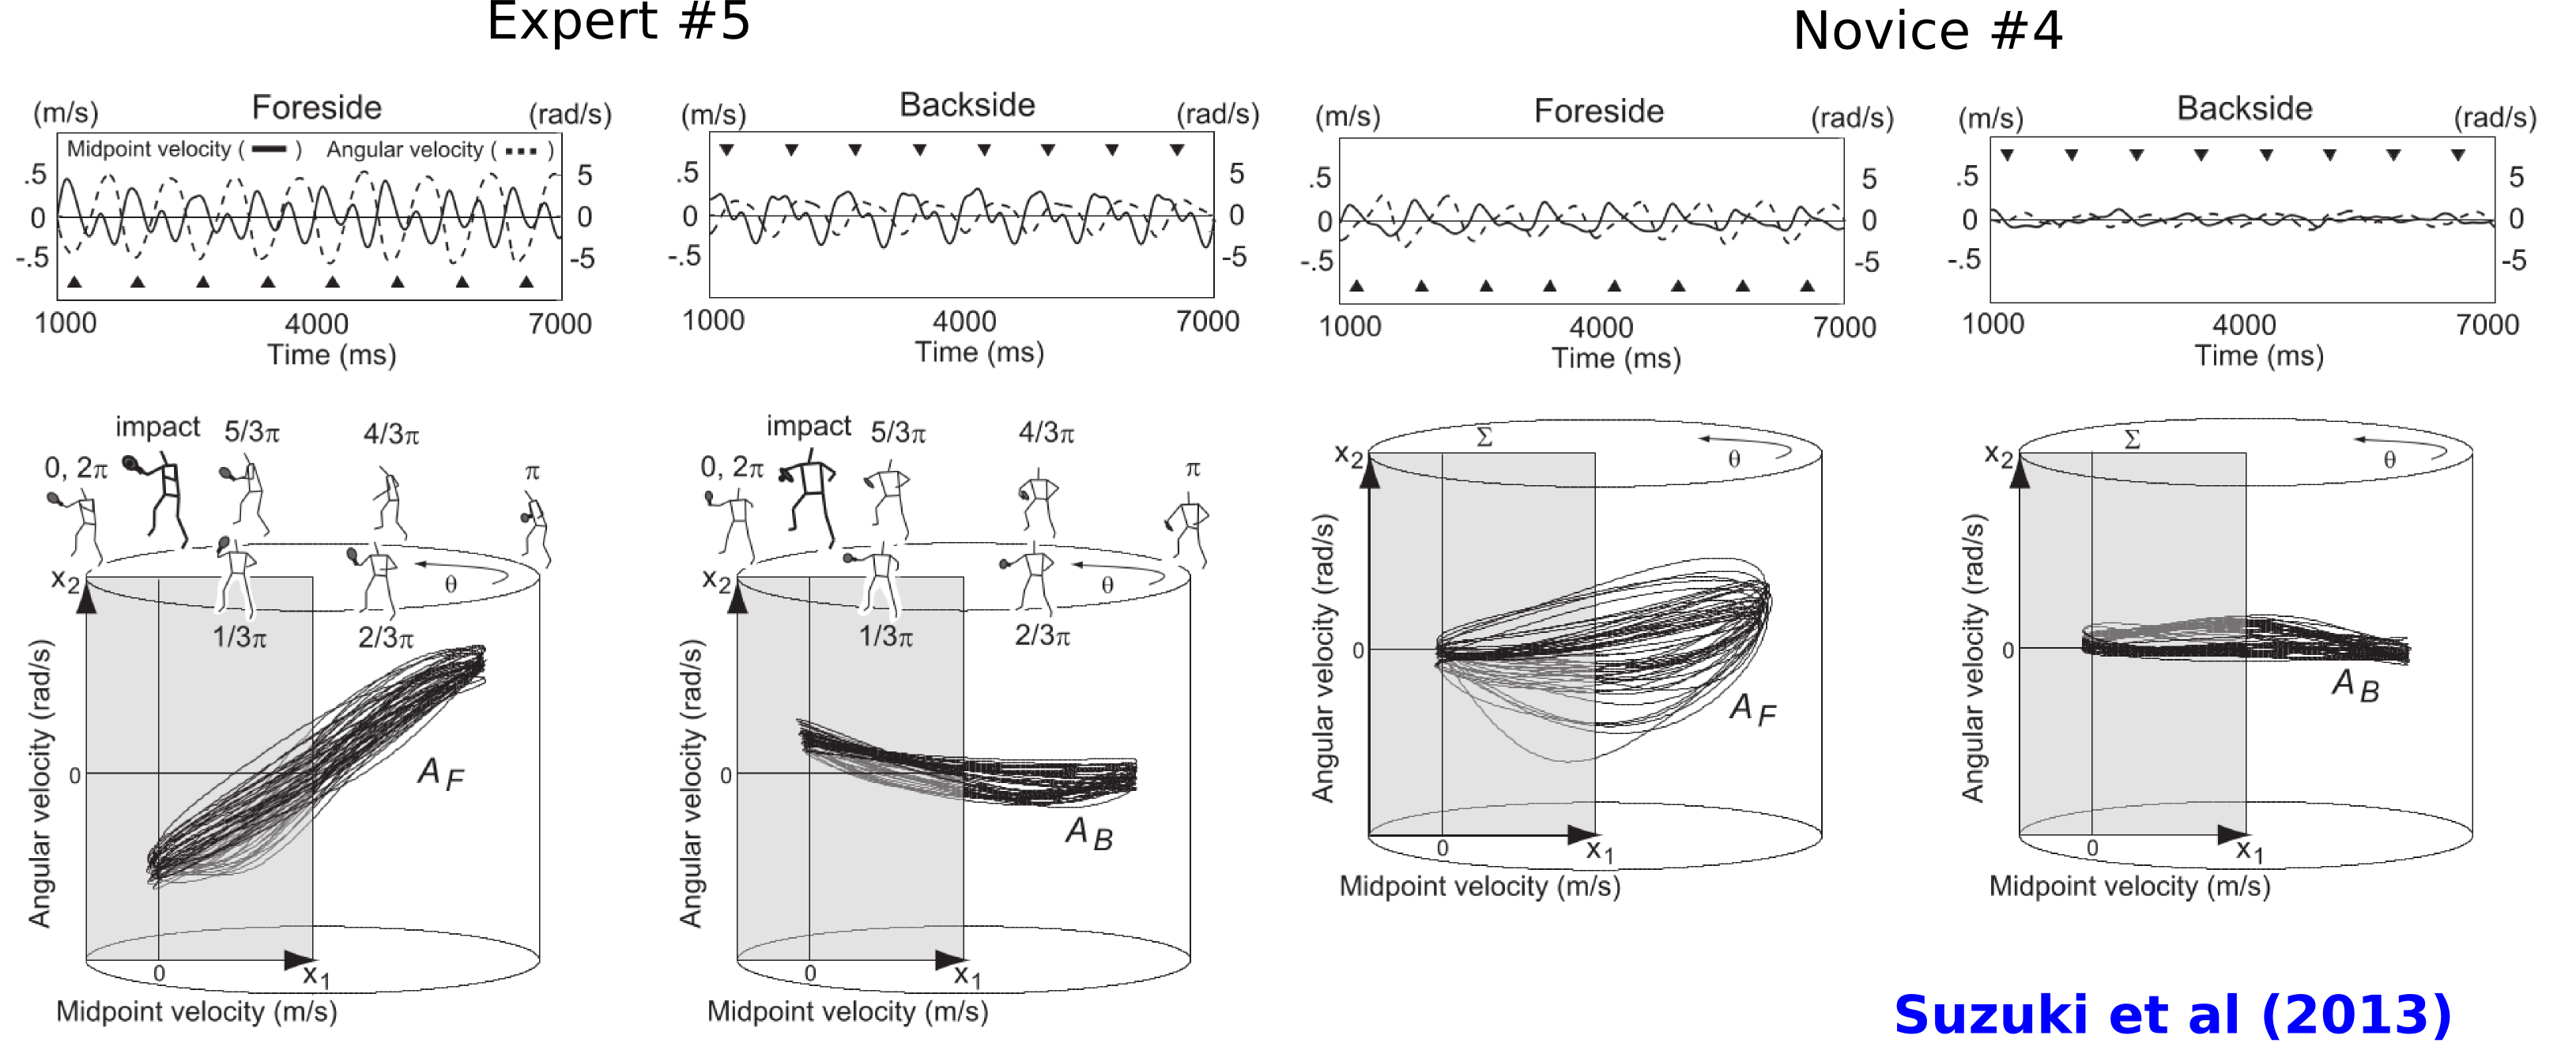
\includegraphics[scale=.2]{dexterity_tennis_suzuky2013}\\
Time series and hyper-cylindrical phase space from Expert \#5 and Novice \#4.
\end{center}
\end{frame}
%---------------------------------------------------


%+++++++++++++++++++++++++++++++++++++++++++++++++++
%+++++++++++++++++++++++++++++++++++++++++++++++++++
\section{Research Questions}

%+++++++++++++++++++++++++++++++++++++++++++++++++++
\begin{frame}
	\frametitle{Research Questions}

    \begin{itemize}
    \item How can phase space representation quantify the dexterity 
          of human activities?
    \item How can we apply Takens's Theorem and Principal Component Analysis
	  to characterise Human Activities?
    \item How do concepts from nonlinear dynamics help us to 
	  characterise dexterity in human activities?
    \end{itemize}

\end{frame}
%---------------------------------------------------


%+++++++++++++++++++++++++++++++++++++++++++++++++++
%+++++++++++++++++++++++++++++++++++++++++++++++++++
\section{State Space Representation}


%+++++++++++++++++++++++++++++++++++++++++++++++++++
\begin{frame}
\frametitle{Reconstructed State Space}
\vspace{-5mm}

\begin{figure}
\centering 
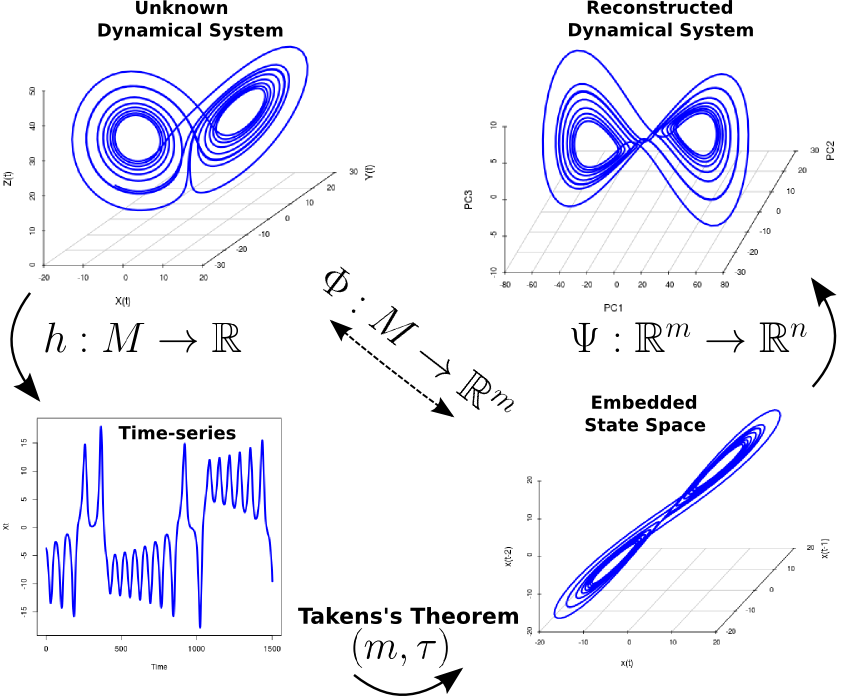
\includegraphics[scale=.35]{takens_theorem_v5} 
\end{figure}

\end{frame}
%---------------------------------------------------






%+++++++++++++++++++++++++++++++++++++++++++++++++++
\begin{frame}
\frametitle{Takens' Theorem (1981)}


According to Takens' Theorem, the reconstructed state space
in  \textbf{$m$ embedding dimension} with  \textbf{ $\tau$ embedding delay}
of the original system is given by 
%the delay coordinate (DC) vector

\begin{eqnarray*} 
\overline{x(t)} = (x(t), x(t - \tau), x(t-2\tau), ... , x (t-(m-1)\tau).
\end{eqnarray*}
 
Takens' Theorem, also knows as time-delay embeddings method, states
that for a large enough $m$ to unfold the attractor and $\tau > 0$ 
chosen to maximize the information content of $x(t)$, this method provides a 
one-to-one reconstruction of the true dimension $k$ system ($\mathbb{R}^k$).

% state space 

% Takens' Theorem, also knows as time-delay embeddings method, is useful 
% when one does not have access to the the true dimension $k$
% state space $\mathbb{R}^k$. Henceforth, it has been demostrated
% that one can obtain a manifold in $\mathbb{R}^m$ that is one-to-one
% and preserves local differential structure.


% One can represent a multidimensional phase
% space of by using the Taken's Theorem.
% 
% Let $o_t$ be the time series, 
% The time-delay reconstruction in $m$ dimensions with the time delay $\tau$
% 
% \begin{eqnarray*} 
% E_t : \mathbb{R}^k \rightarrow \mathbb{R}^m 
% \end{eqnarray*}

% It's natural to think that if $g'(c)>0$ then $g$ must be ``increasing at $x=c$.'' 
% \pause But what does ``increasing at $x=c$'' really mean?
% \pause 
% Taken's Method

% \begin{dfn} % We created the proclamation dfn near the start of the document.
% A function $g$ is \emph{increasing at $x=c$} if there 
% is an open interval $I=(c-\delta,c+\delta)$ such that \pause if $x_1, x_2\in I$, \pause then $x_1<x_2\Rightarrow \pause g(x_1)<g(x_2)$.
% \end{dfn}
\end{frame}
%---------------------------------------------------




%+++++++++++++++++++++++++++++++++++++++++++++++++++
\begin{frame}
\frametitle{Minimum embedding parameters}

\textbf{Cao (1997)} proposed a method 
based on the false neighbor method
to determine the minimum embedding dimmension
from time-series based on Taken's theorem.

% \textbf{Fraser et al (1985)}  used the mutual information method 
% for the choice of the delay embedding.

\begin{figure}
\centering 
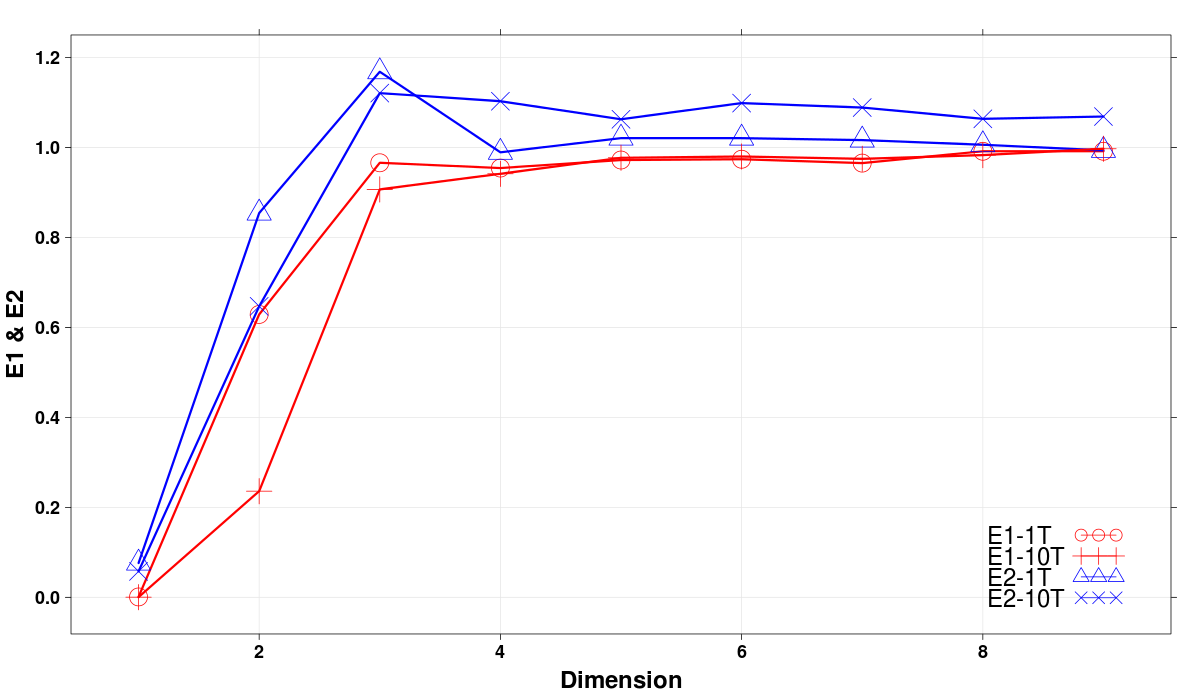
\includegraphics[scale=0.15]{e1e2cao1997} \\
The values E1 and E2 from Lorenz attractor \textbf{Cao (1997)}
\end{figure}
\end{frame}
%---------------------------------------------------





%+++++++++++++++++++++++++++++++++++++++++++++++++++
\begin{frame}
\frametitle{Phase Space Reconstruction}

\begin{figure}
 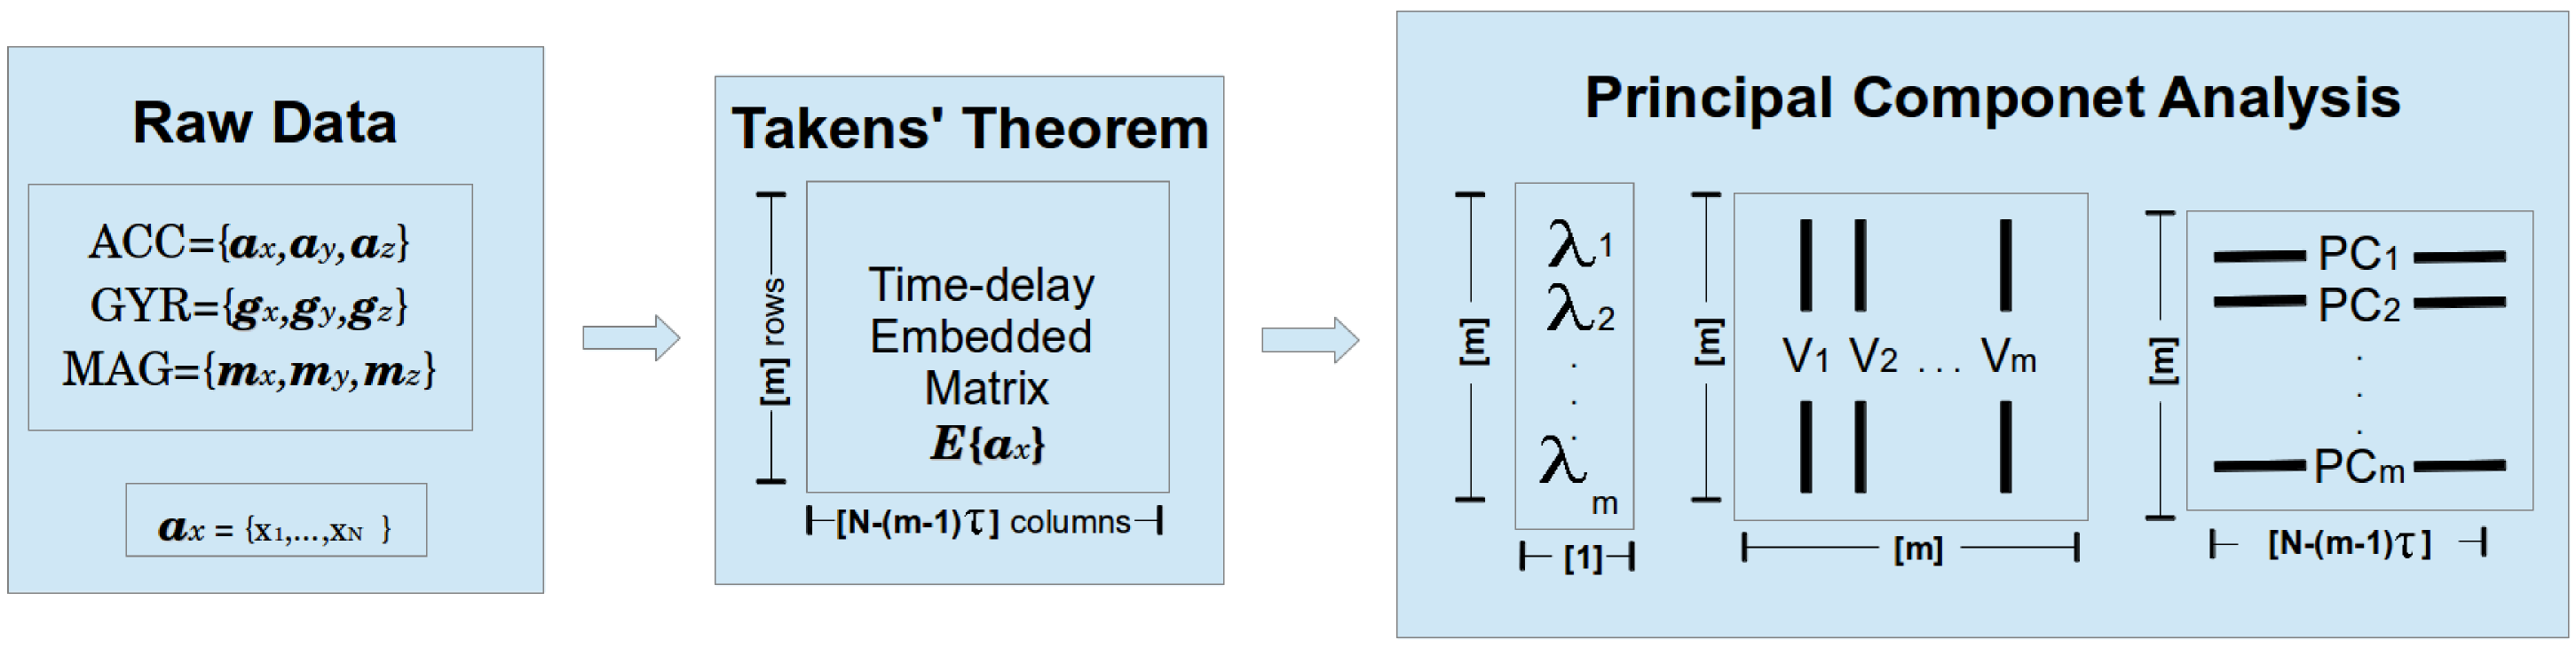
\includegraphics[scale=.23]{diagram_v9} \\
%\caption{Time series of the Lorenz System and 2D manifolds}
\end{figure} 
 
\end{frame}

% 



%+++++++++++++++++++++++++++++++++++++++++++++++++++
 \begin{frame}
 \frametitle{Time-Delay Embedding Example }
   
  \begin{columns}[onlytextwidth]
    \begin{column}{0.3\textwidth}
Lorenz System
 \begin{eqnarray*} 
  \frac{dx}{dt} &=&\sigma (x-y), \\
  \frac{dx}{dt} &=&x (\rho -z) - y, \\ 
  \frac{dx}{dt} &=&xy - \beta z.
 \end{eqnarray*}
 \end{column} 
  
  \begin{column}{0.63\textwidth}
       \begin{figure}
 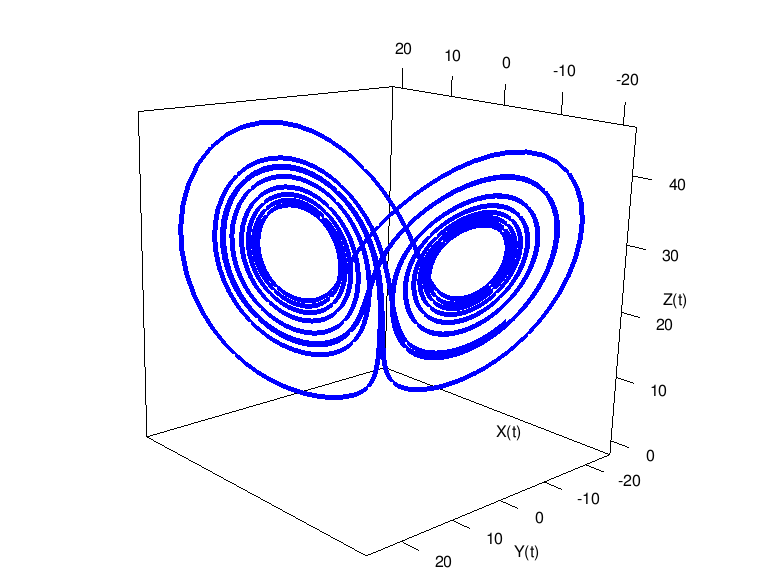
\includegraphics[scale=.25]{lorenzattractor}
  \caption{$\sigma=10$, $\rho=28$ and $\beta=3/8$}
       \end{figure}
     \end{column}
  \end{columns}
 \end{frame}



%+++++++++++++++++++++++++++++++++++++++++++++++++++
%%%%%%%%%%%%%%%
%%ANIMATION in evince
\begin{frame}
\frametitle{Time-Delay Embedding Example}
\vspace{-9mm}
\begin{columns}[onlytextwidth]
  \begin{column}{0.5\textwidth}
\begin{figure}
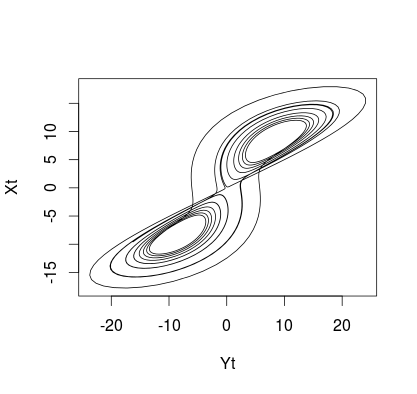
\includegraphics[scale=.3]{XY} 
\caption{Original Manifold}
\end{figure} 
\end{column} 

\begin{column}{0.5\textwidth}

\begin{figure}
\multiinclude[format=png,graphics={scale=0.25}]{images_frames_for_TAU/join} 
% 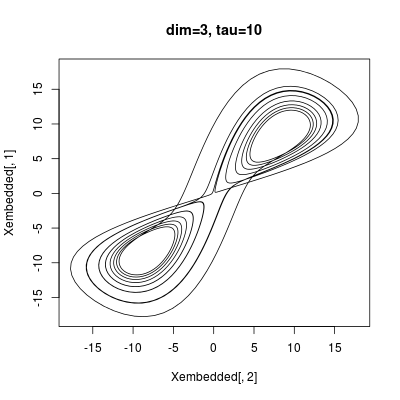
\includegraphics[scale=0.3]{images_frames_for_TAU/manifold_d3_t-10}
\caption{Reconstructed Manifold}
\end{figure}
\end{column}
\end{columns}
\end{frame}










%+++++++++++++++++++++++++++++++++++++++++++++++++++
%+++++++++++++++++++++++++++++++++++++++++++++++++++
\section{Preliminary Experiments}

% %+++++++++++++++++++++++++++++++++++++++++++++++++++
% \begin{frame}
% \frametitle{My goals this month}
% 
% 
%    \begin{itemize}	
%       \item Determine the technique(s) to quantify the dexterity of 
%         Salsa Dancers based on the analysis of the reconstructed state space.
%       \item Submit a paper in The International Symposium on Wearable Computers (ISWC).
%         Deadline: April 10th, 2015.
%     \end{itemize}
% 
% 
% \end{frame}
% %---------------------------------------------------

%+++++++++++++++++++++++++++++++++++++++++++++++++++
\begin{frame}
\frametitle{DECIMUS Class in C++}

\begin{figure}
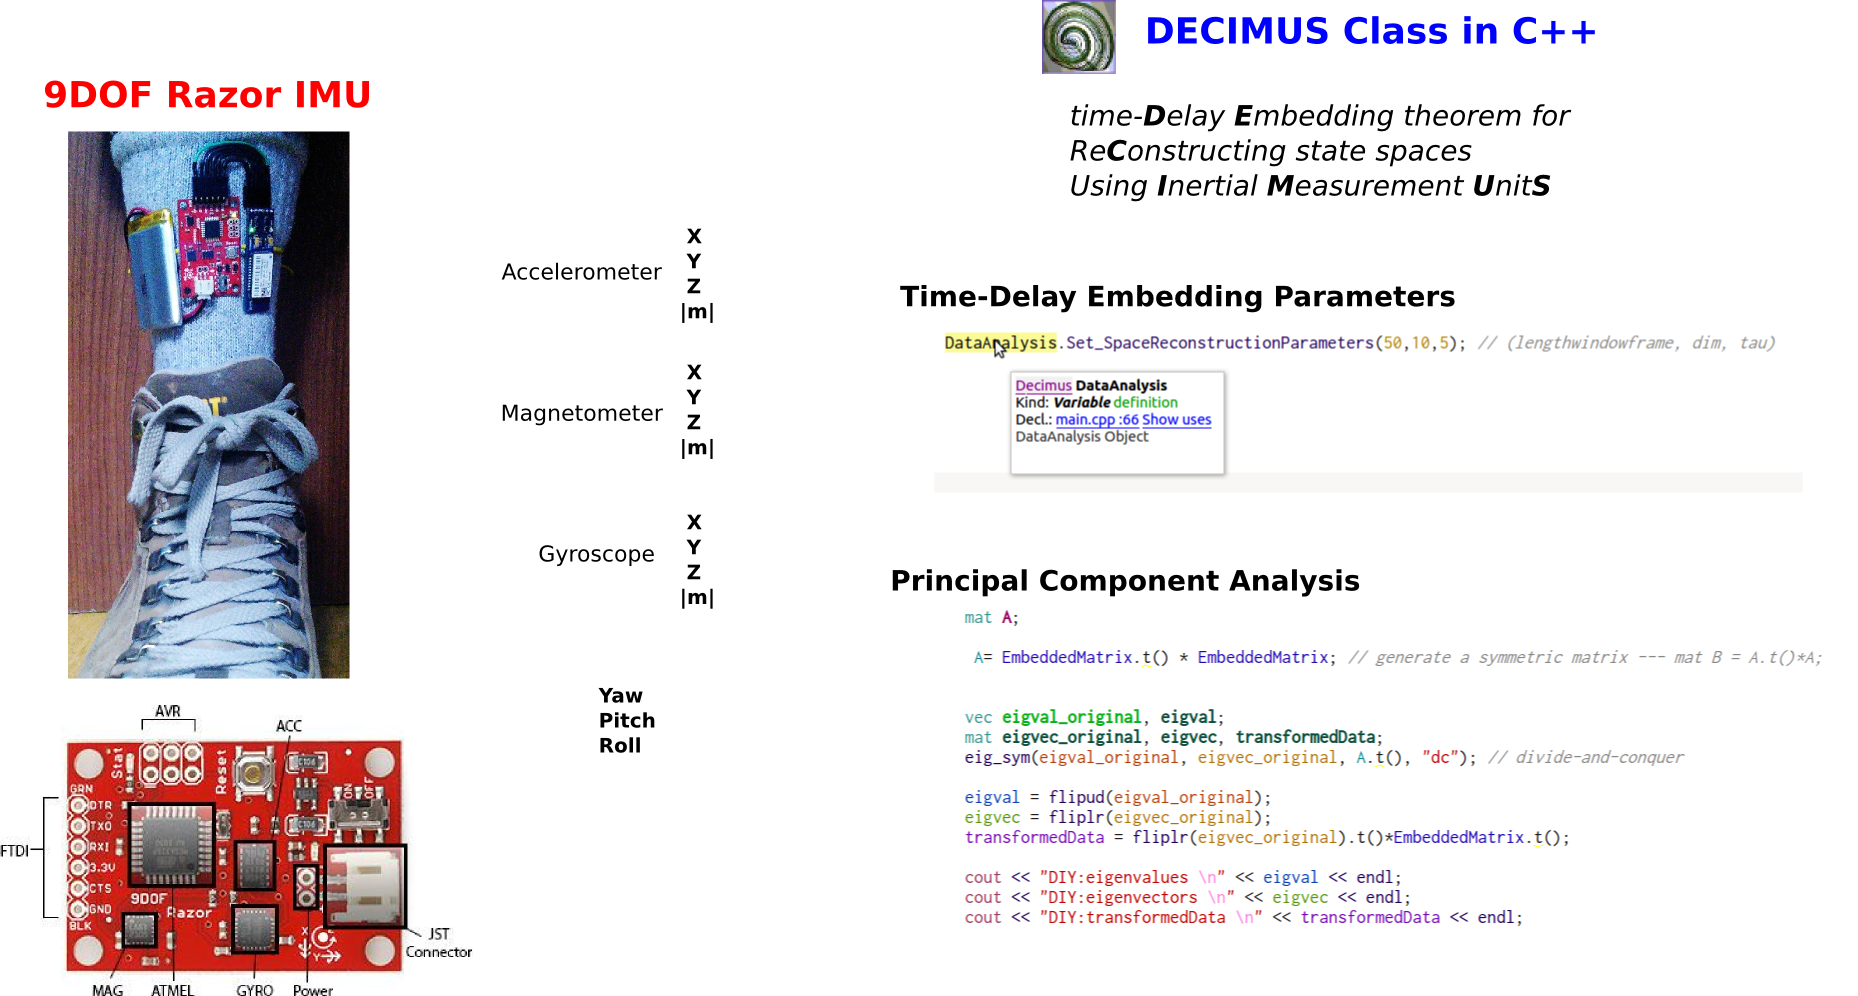
\includegraphics[scale=0.2]{procedure} \\
IMU, Axes and C++ Class
\end{figure}  
\end{frame}

 


%+++++++++++++++++++++++++++++++++++++++++++++++++++
\begin{frame}
\frametitle{Sawing  with a toolbox saw}
\vspace{-5mm}

 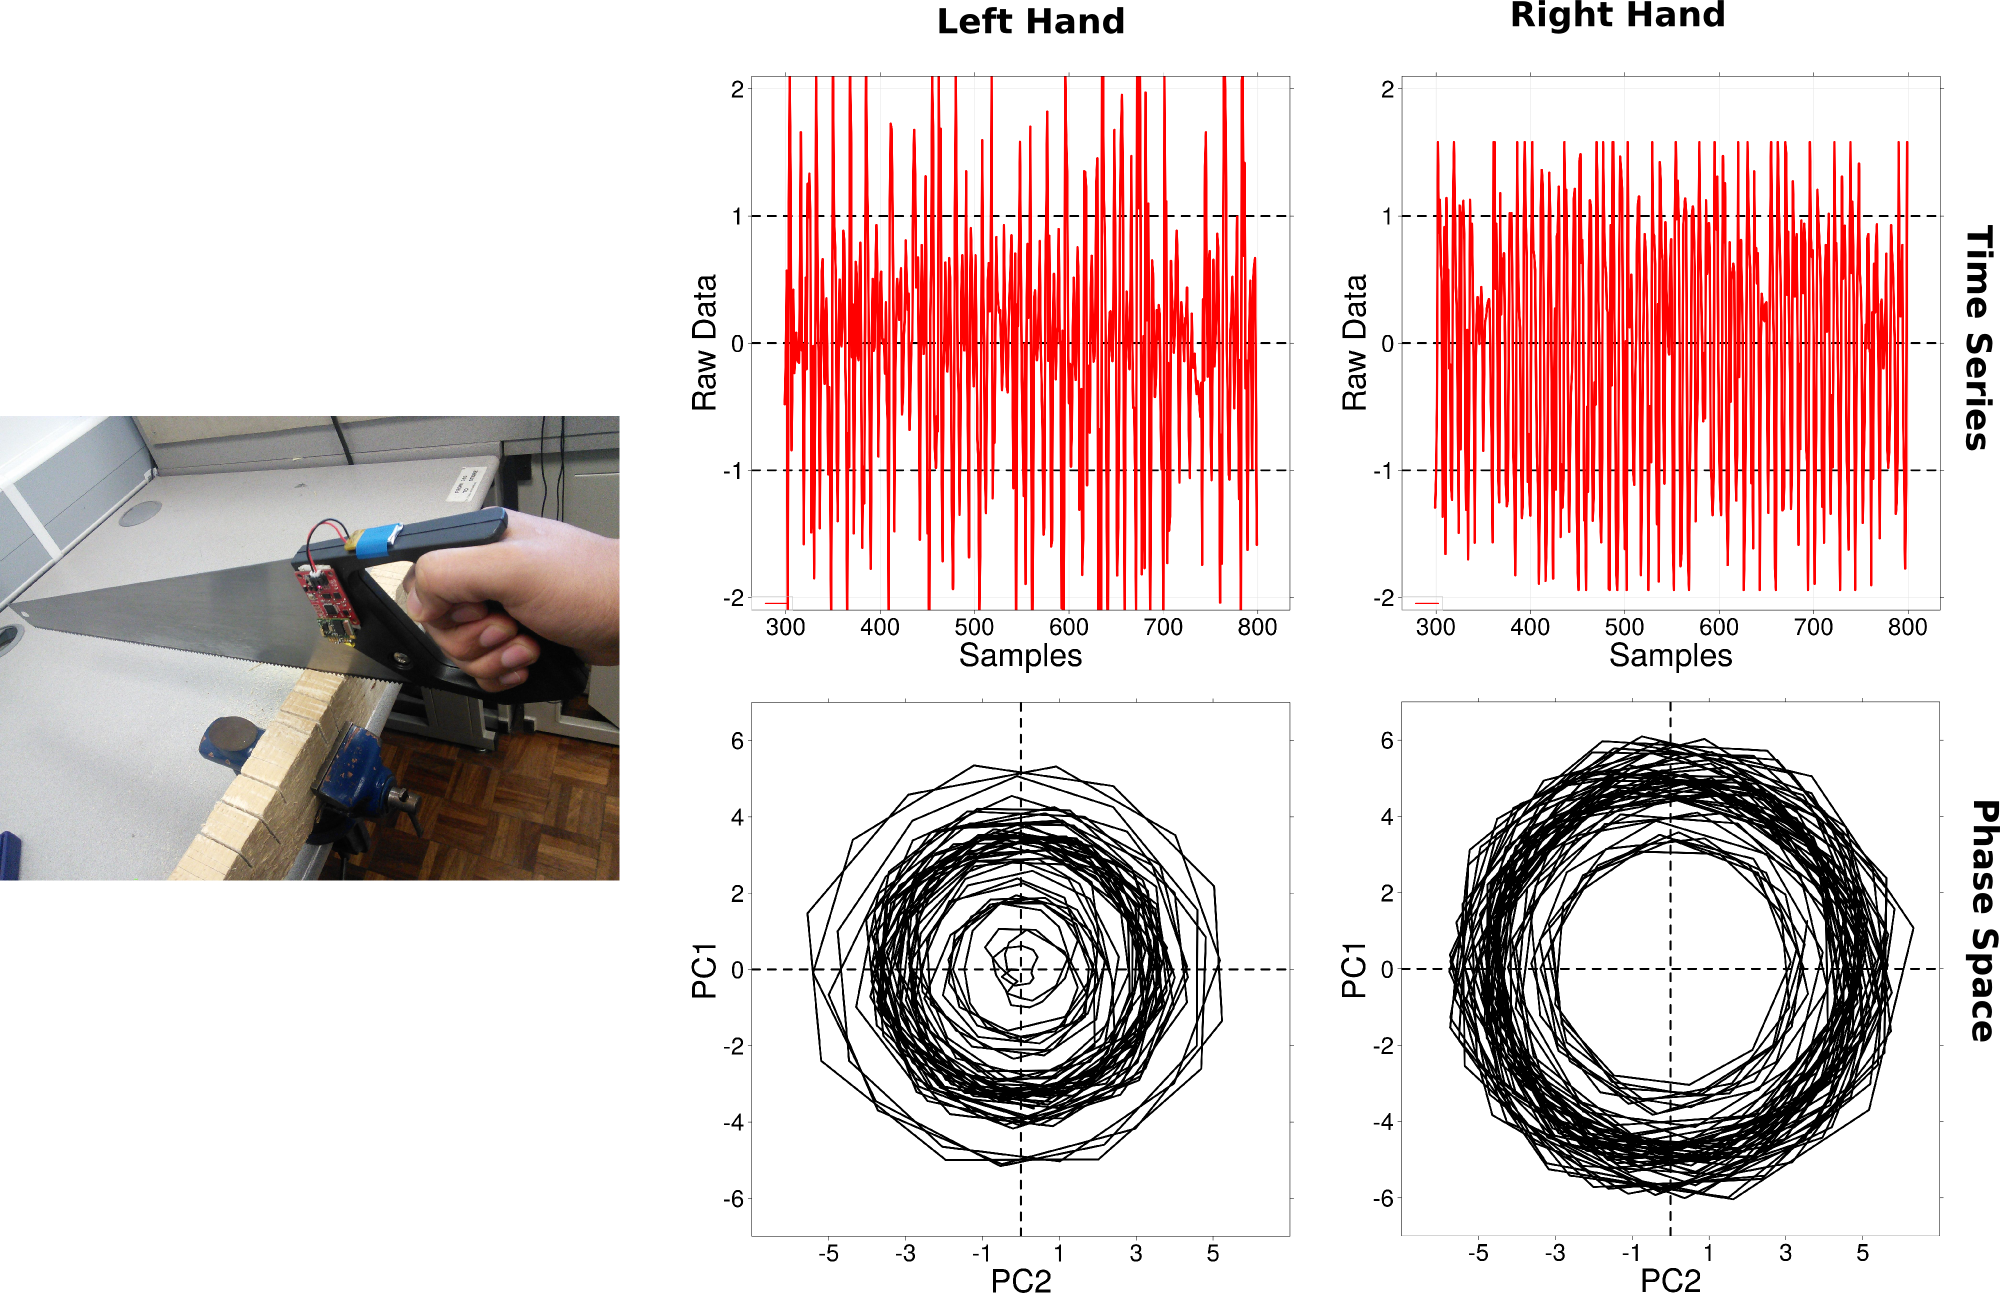
\includegraphics[scale=.045]{toolboxsaw} 

\end{frame}
%---------------------------------------------------

%+++++++++++++++++++++++++++++++++++++++++++++++++++
\begin{frame}
\frametitle{Sawing with a hack saw}
\vspace{-5mm}

 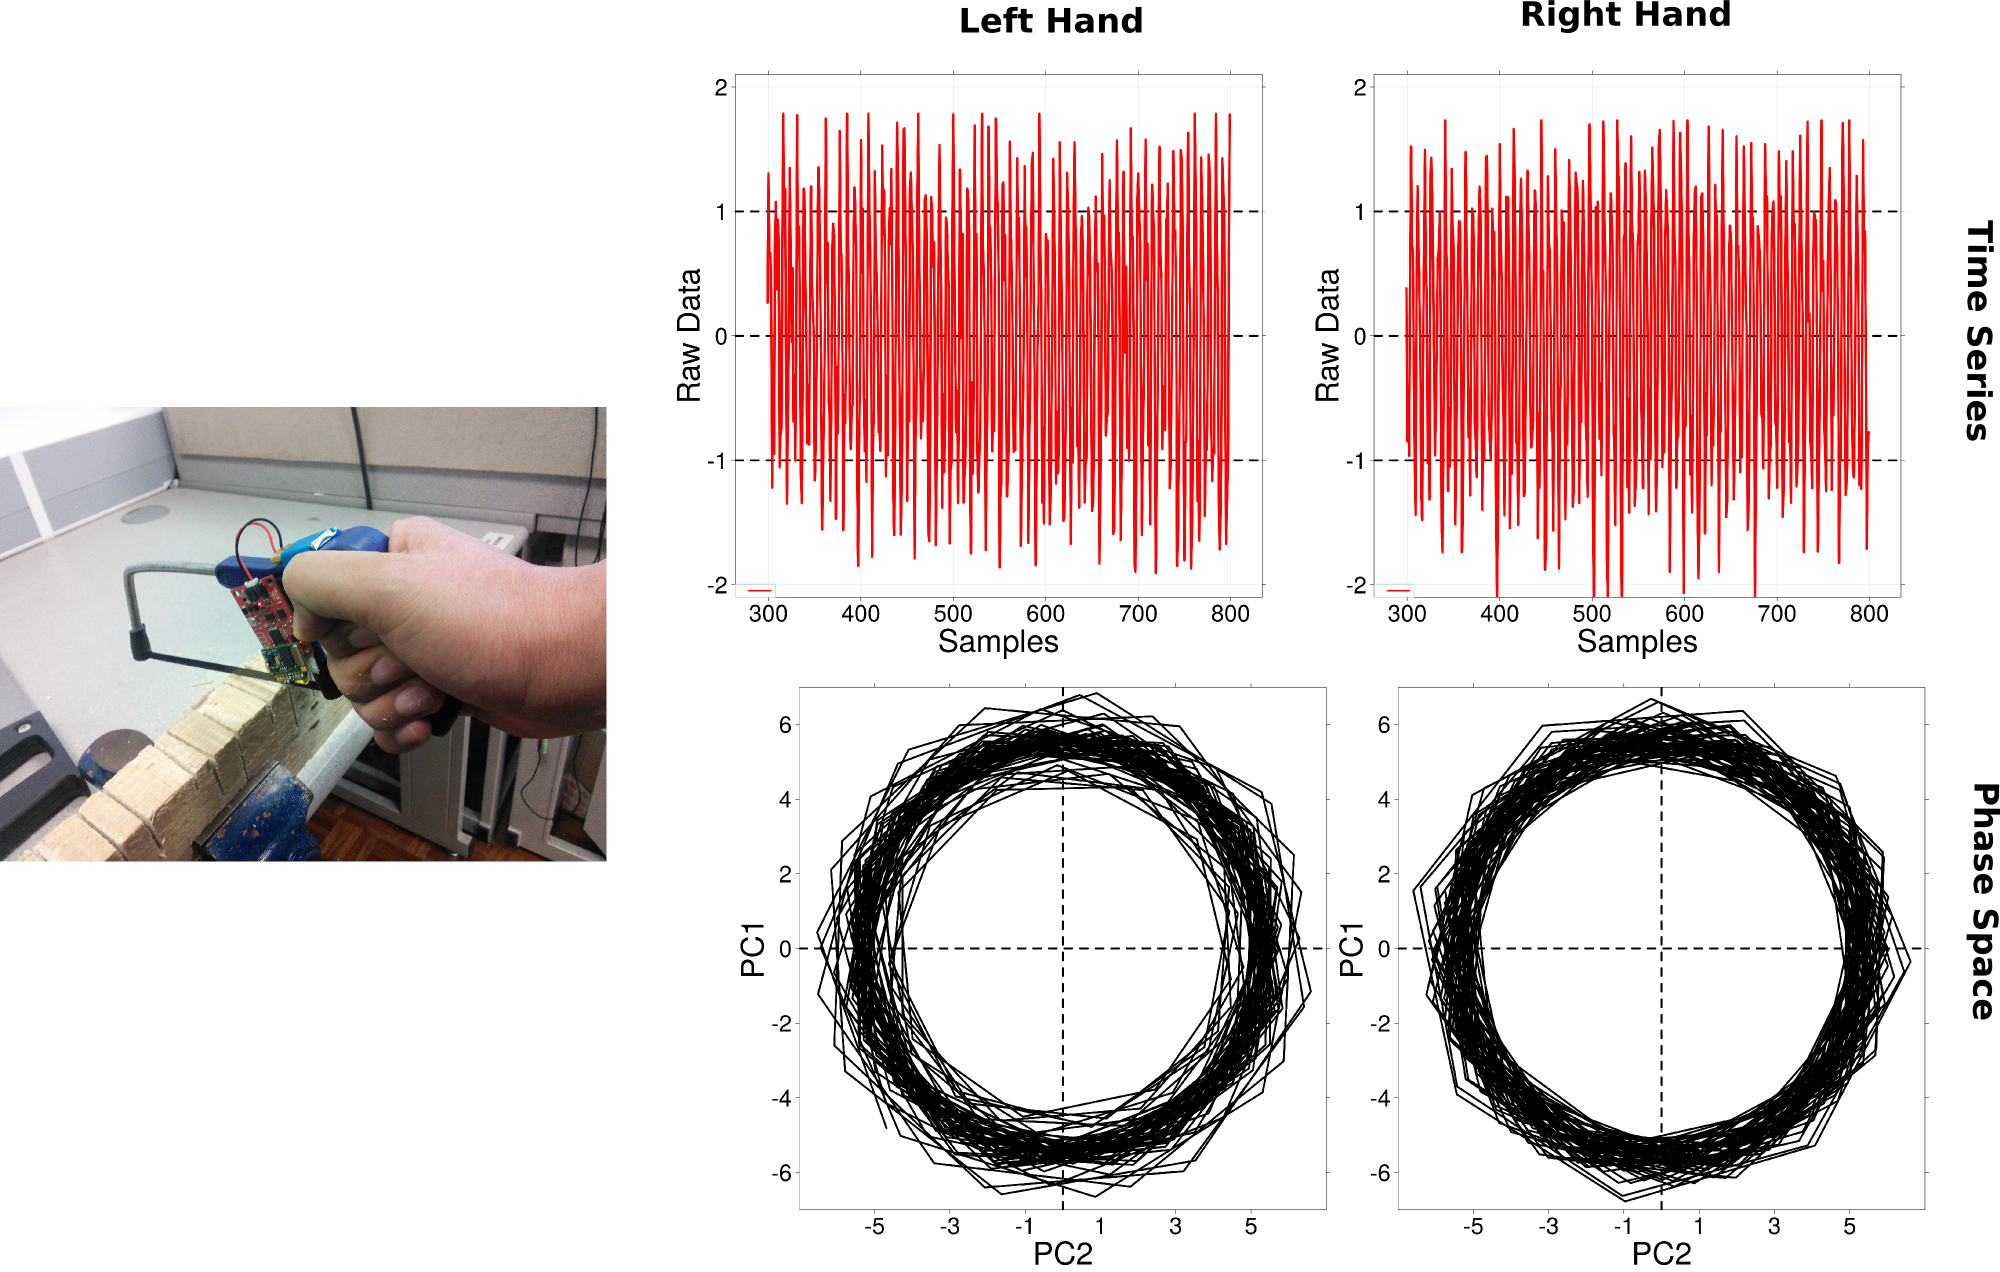
\includegraphics[scale=.045]{hacksaw} 

\end{frame}
%---------------------------------------------------







%+++++++++++++++++++++++++++++++++++++++++++++++++++
\begin{frame}
\frametitle{Quantifying Dexterity in Dance}
\vspace{-0.6cm}
\begin{figure}
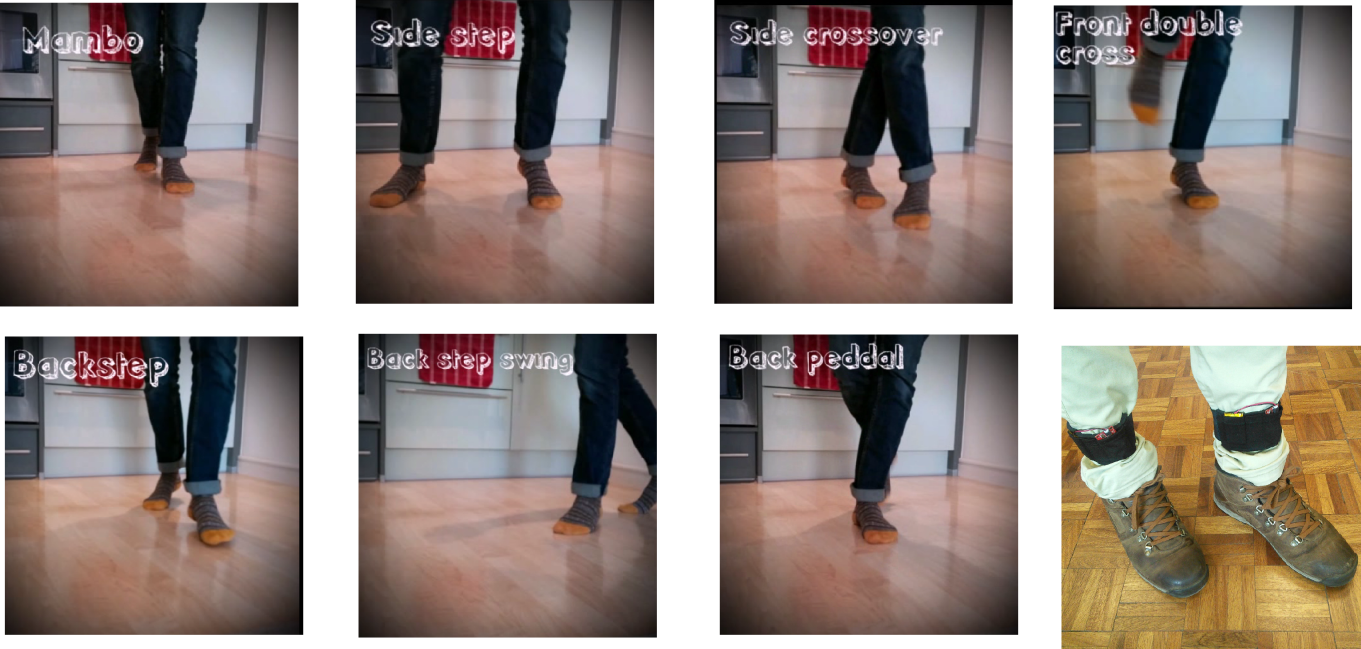
\includegraphics[scale=0.5]{beginner_salsa_steps_01} \\

\end{figure}  
\end{frame}


%+++++++++++++++++++++++++++++++++++++++++++++++++++
\begin{frame}
\frametitle{Phase Spaces for Dancing}
\vspace{-0.6cm}
\begin{figure}
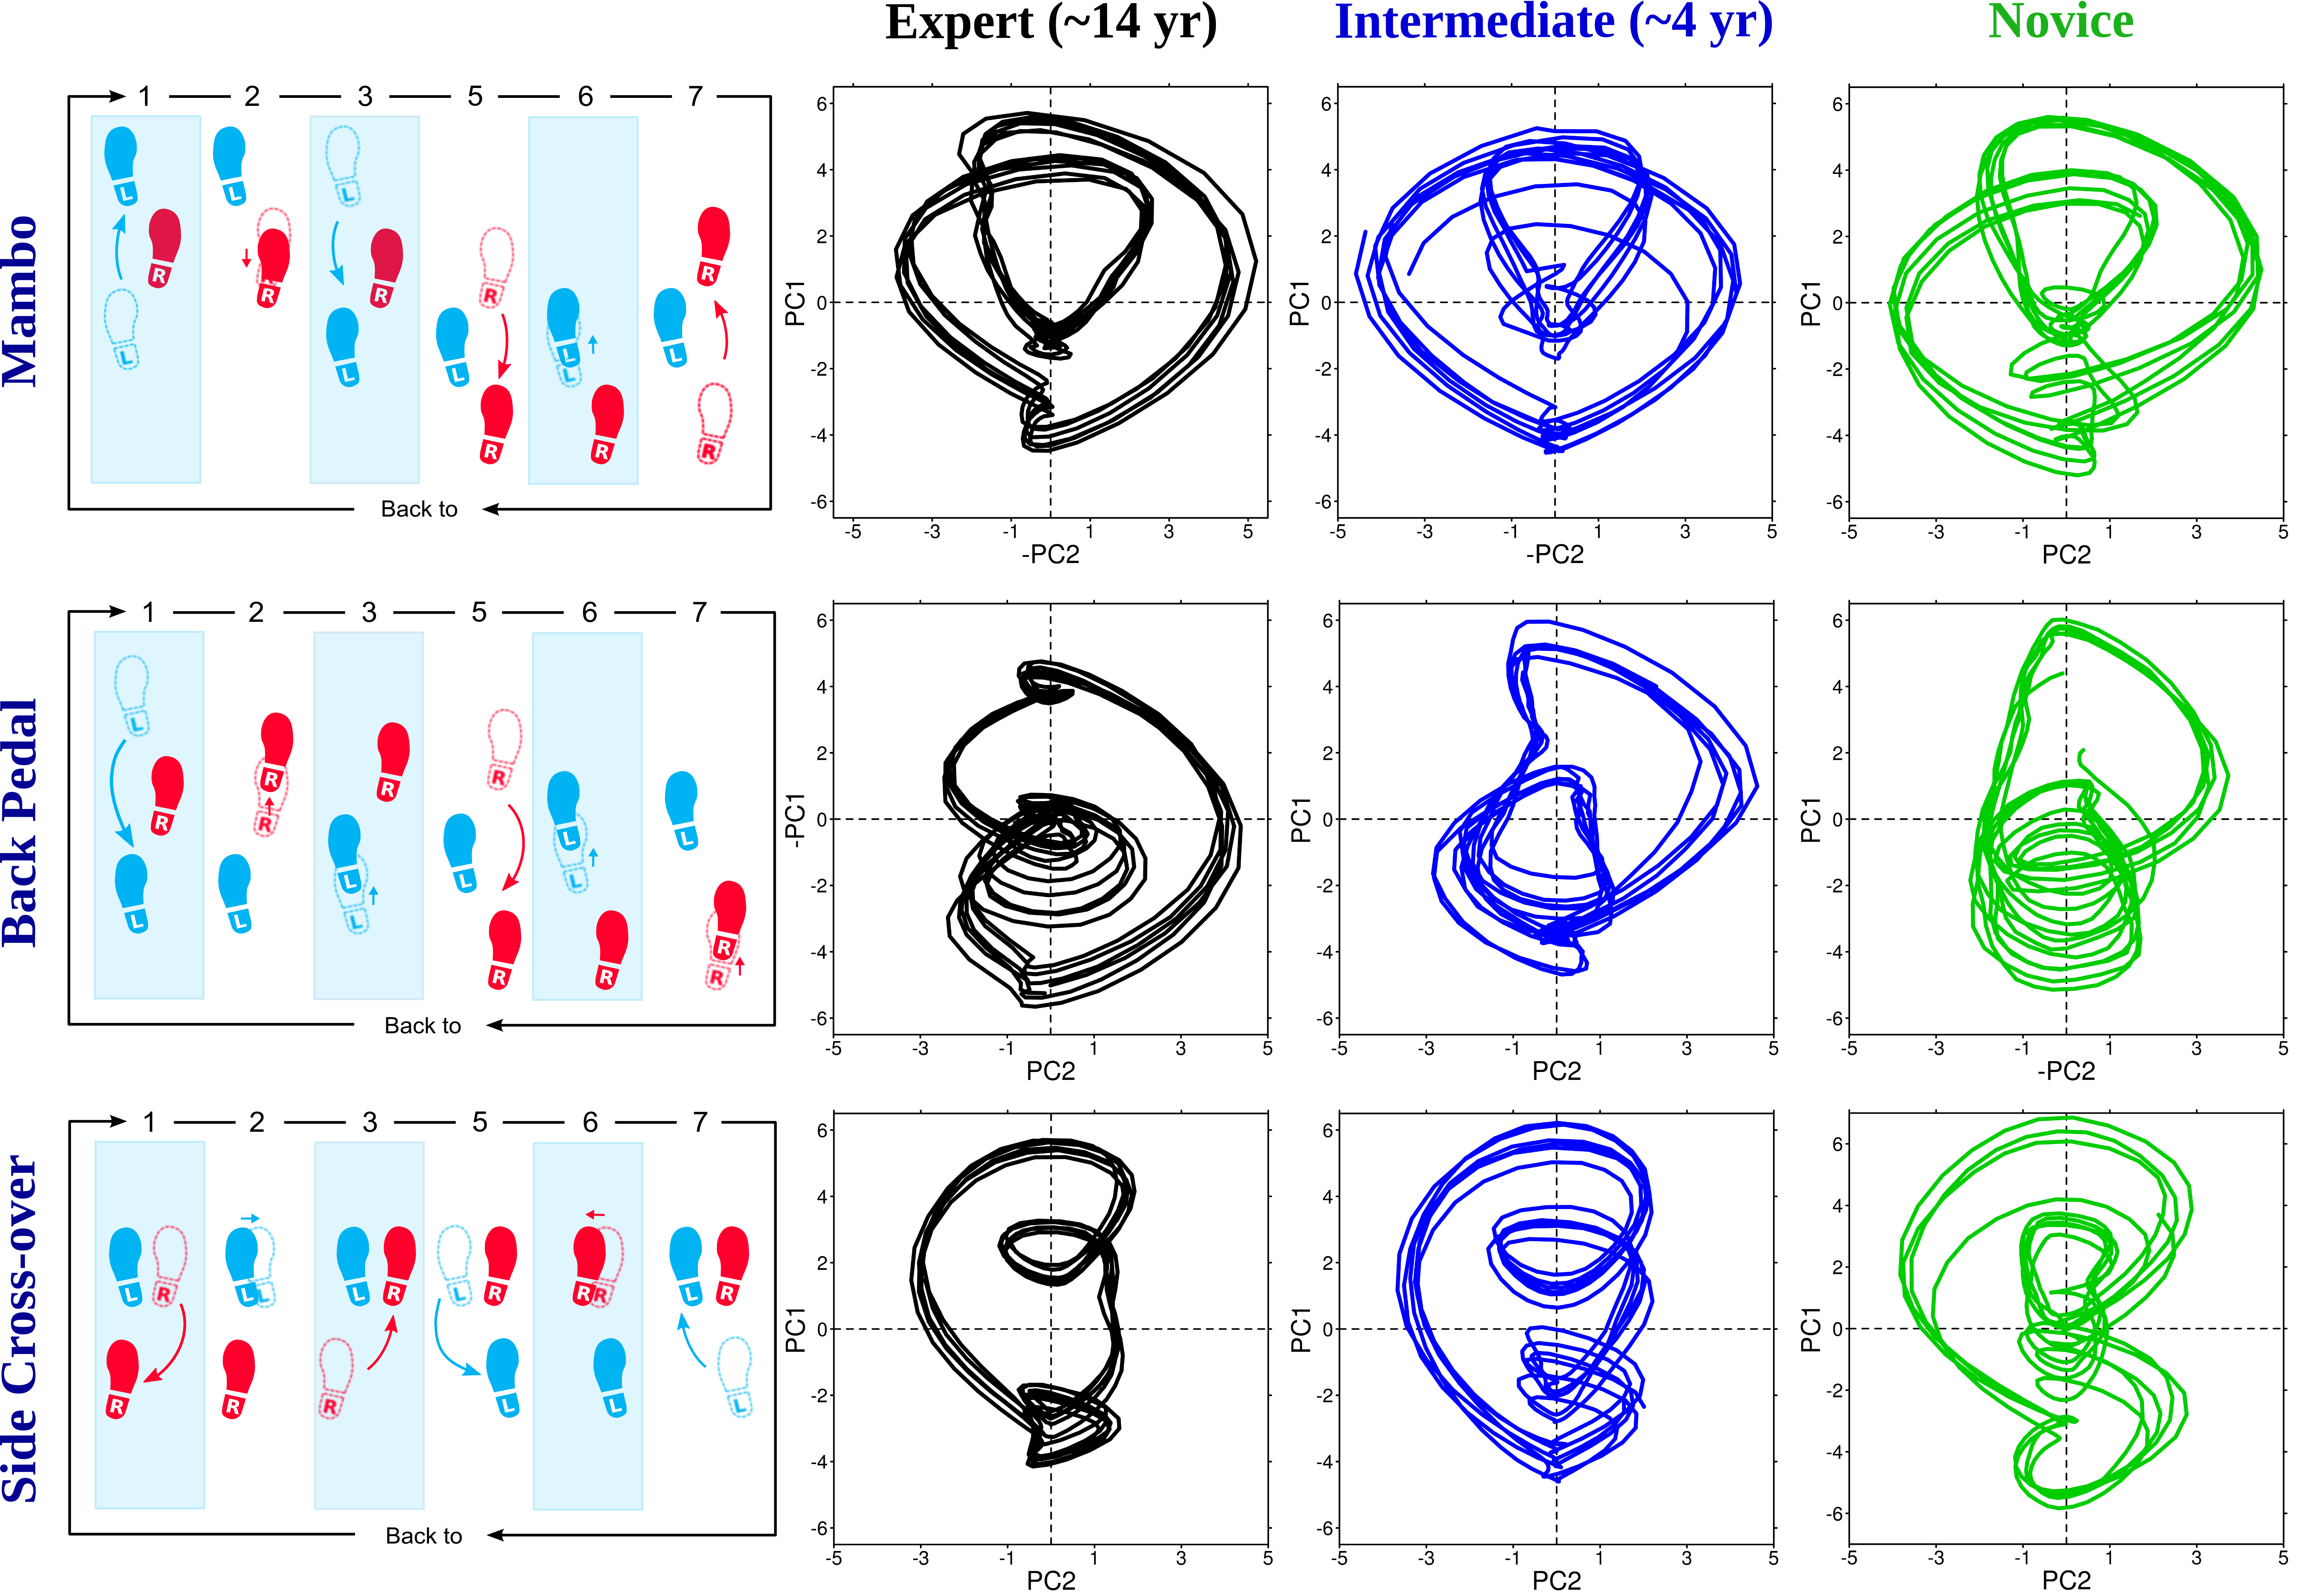
\includegraphics[scale=0.029]{results_v11} \\
\end{figure}  
\end{frame}

% %+++++++++++++++++++++++++++++++++++++++++++++++++++
% \begin{frame}
% \frametitle{$E1(d)$ and $E2(d)$ values}
% \vspace{-0.6cm}
% \begin{figure}
% \includegraphics[scale=0.07]{ev_gyr} \\
% 
% \end{figure}  
% \end{frame}
% 
% 
% %+++++++++++++++++++++++++++++++++++++++++++++++++++
% \begin{frame}
% \frametitle{$E1(d)$ and $E2(d)$ values}
% \vspace{-0.6cm}
% \begin{figure}
% \includegraphics[scale=0.07]{ev_mag} \\
% 
% \end{figure}  
% \end{frame}
% 



% 
% %+++++++++++++++++++++++++++++++++++++++++++++++++++
% \begin{frame}
% \frametitle{Percentages of variances}
% \vspace{-0.6cm}
% \begin{figure}
% 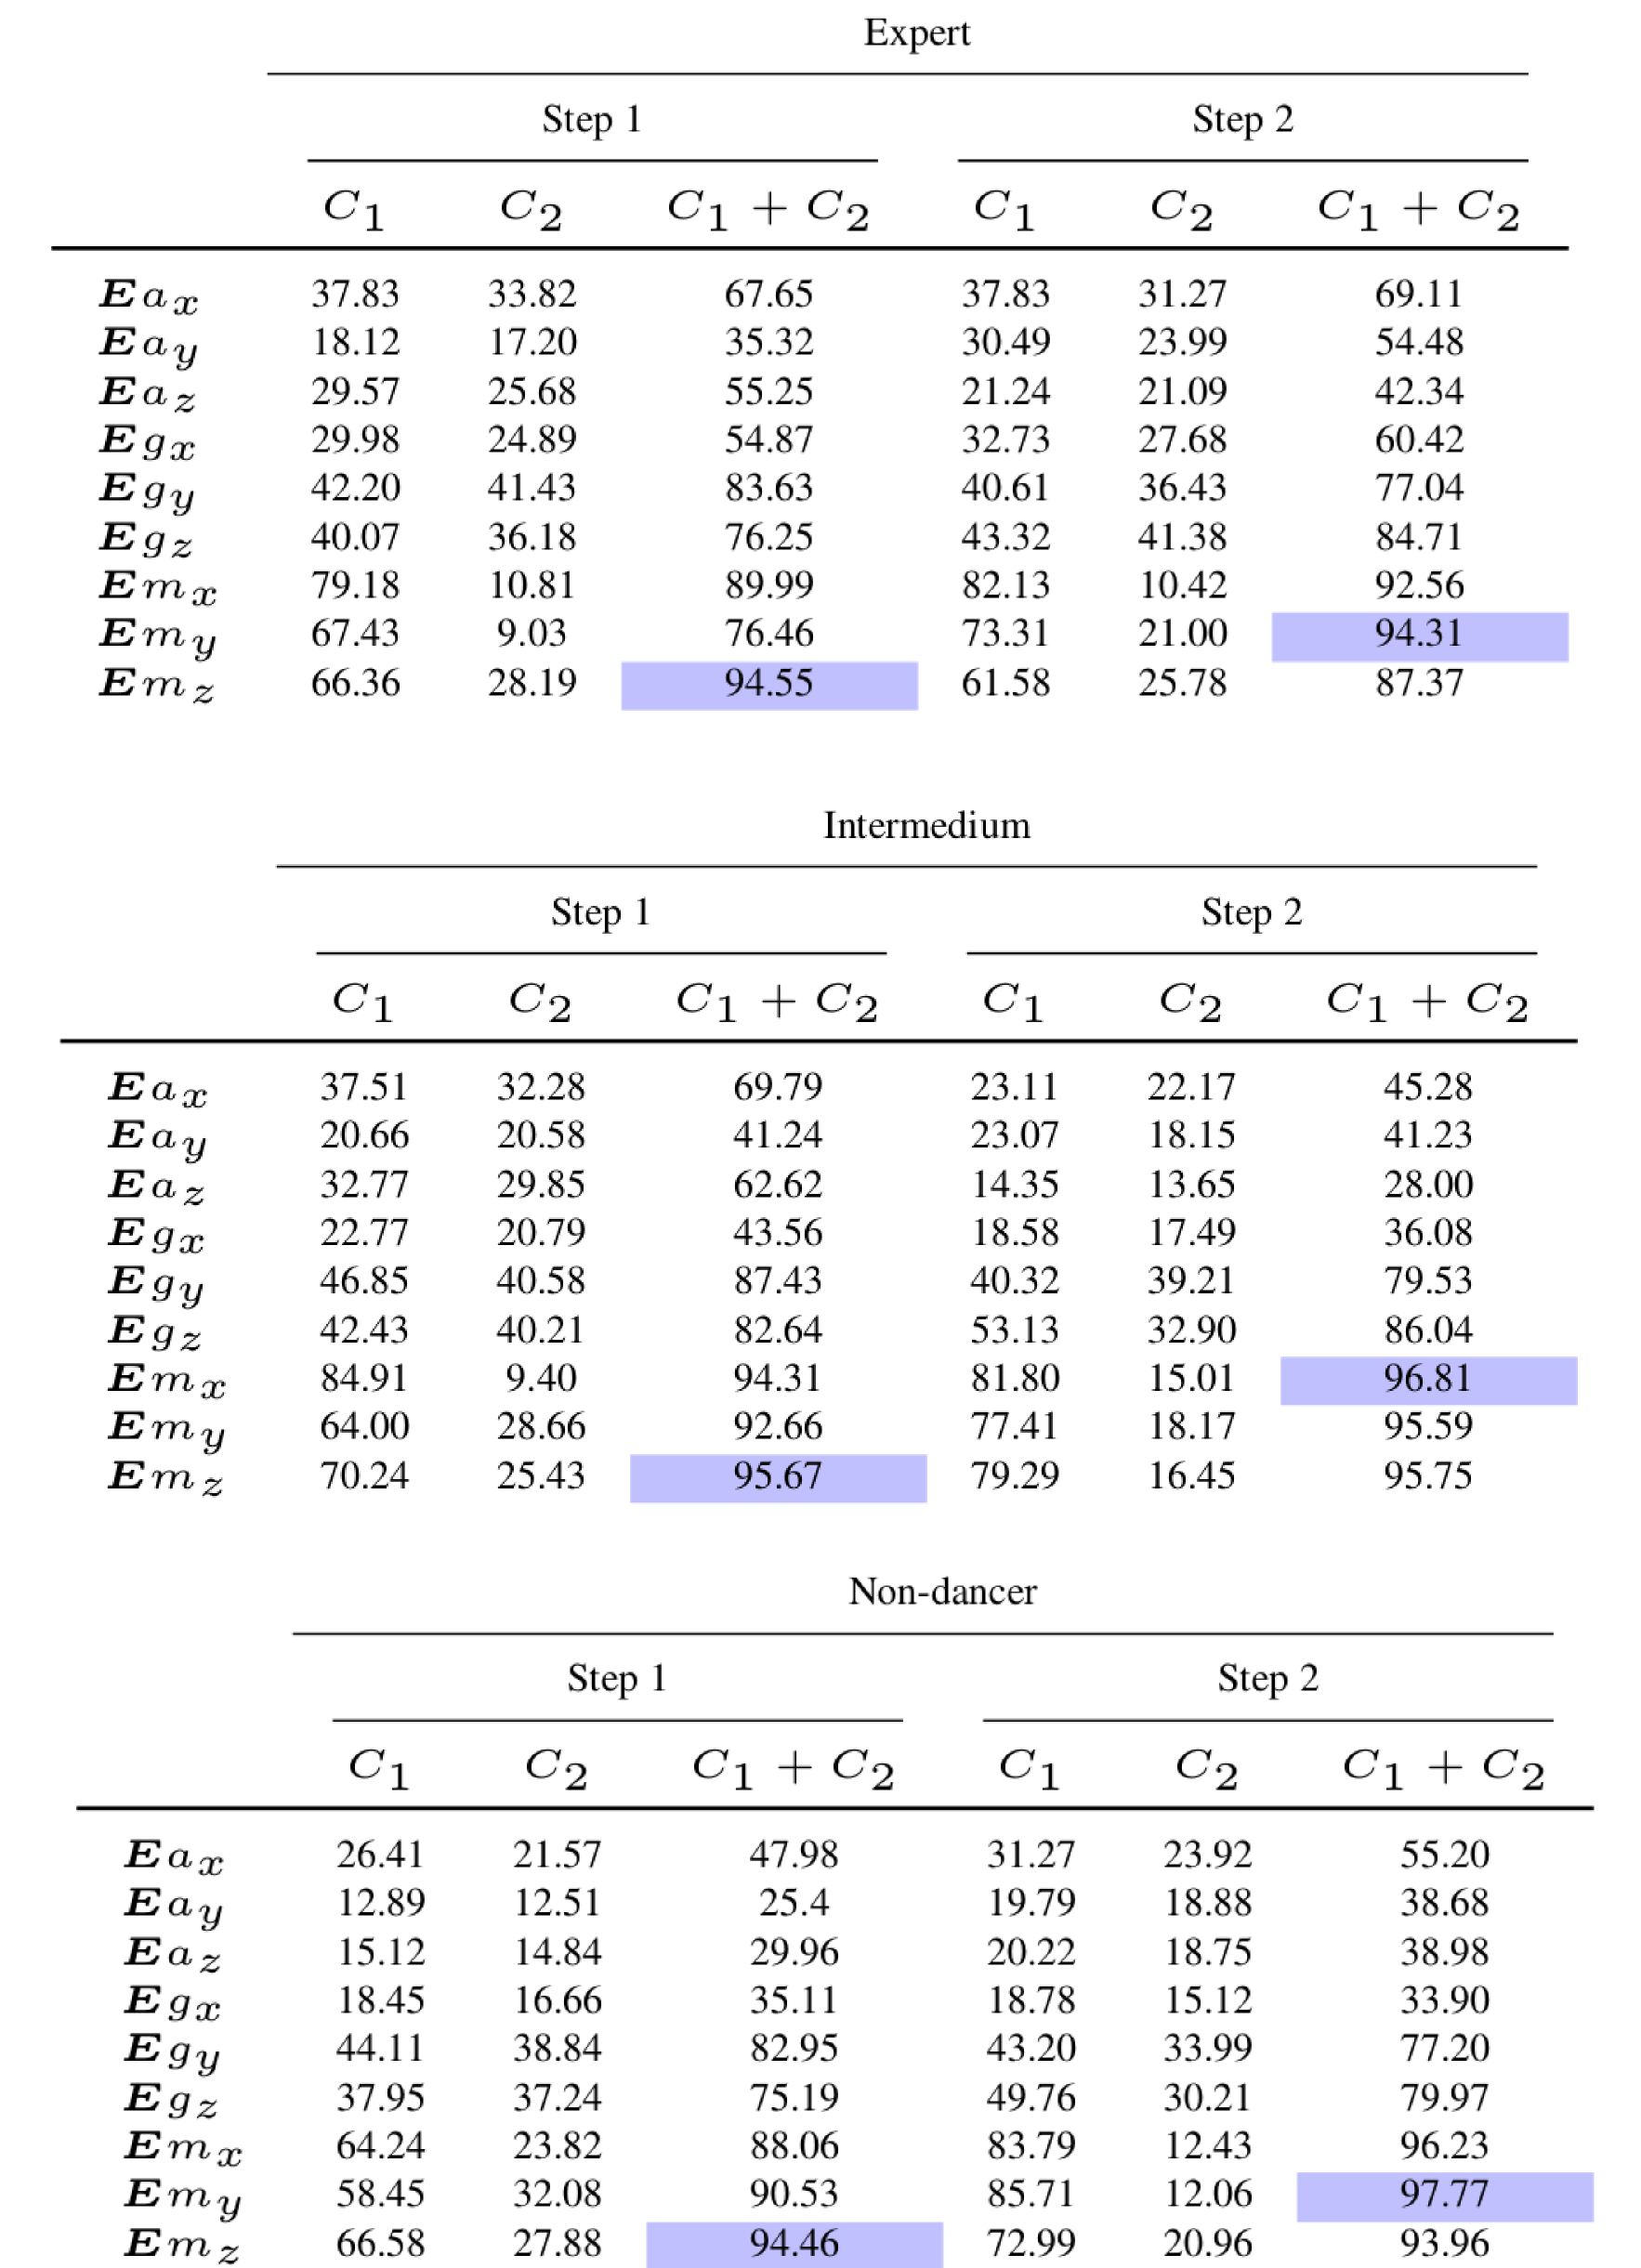
\includegraphics[scale=0.15]{tables_v1} \\
% 
% \end{figure}  
% \end{frame}
% 
% 
% 
% 



% 
% 
% %+++++++++++++++++++++++++++++++++++++++++++++++++++
% \begin{frame}
% \frametitle{2-D reconstructed state spaces (RSS)}
% \vspace{-0.6cm}
% \begin{figure}
% 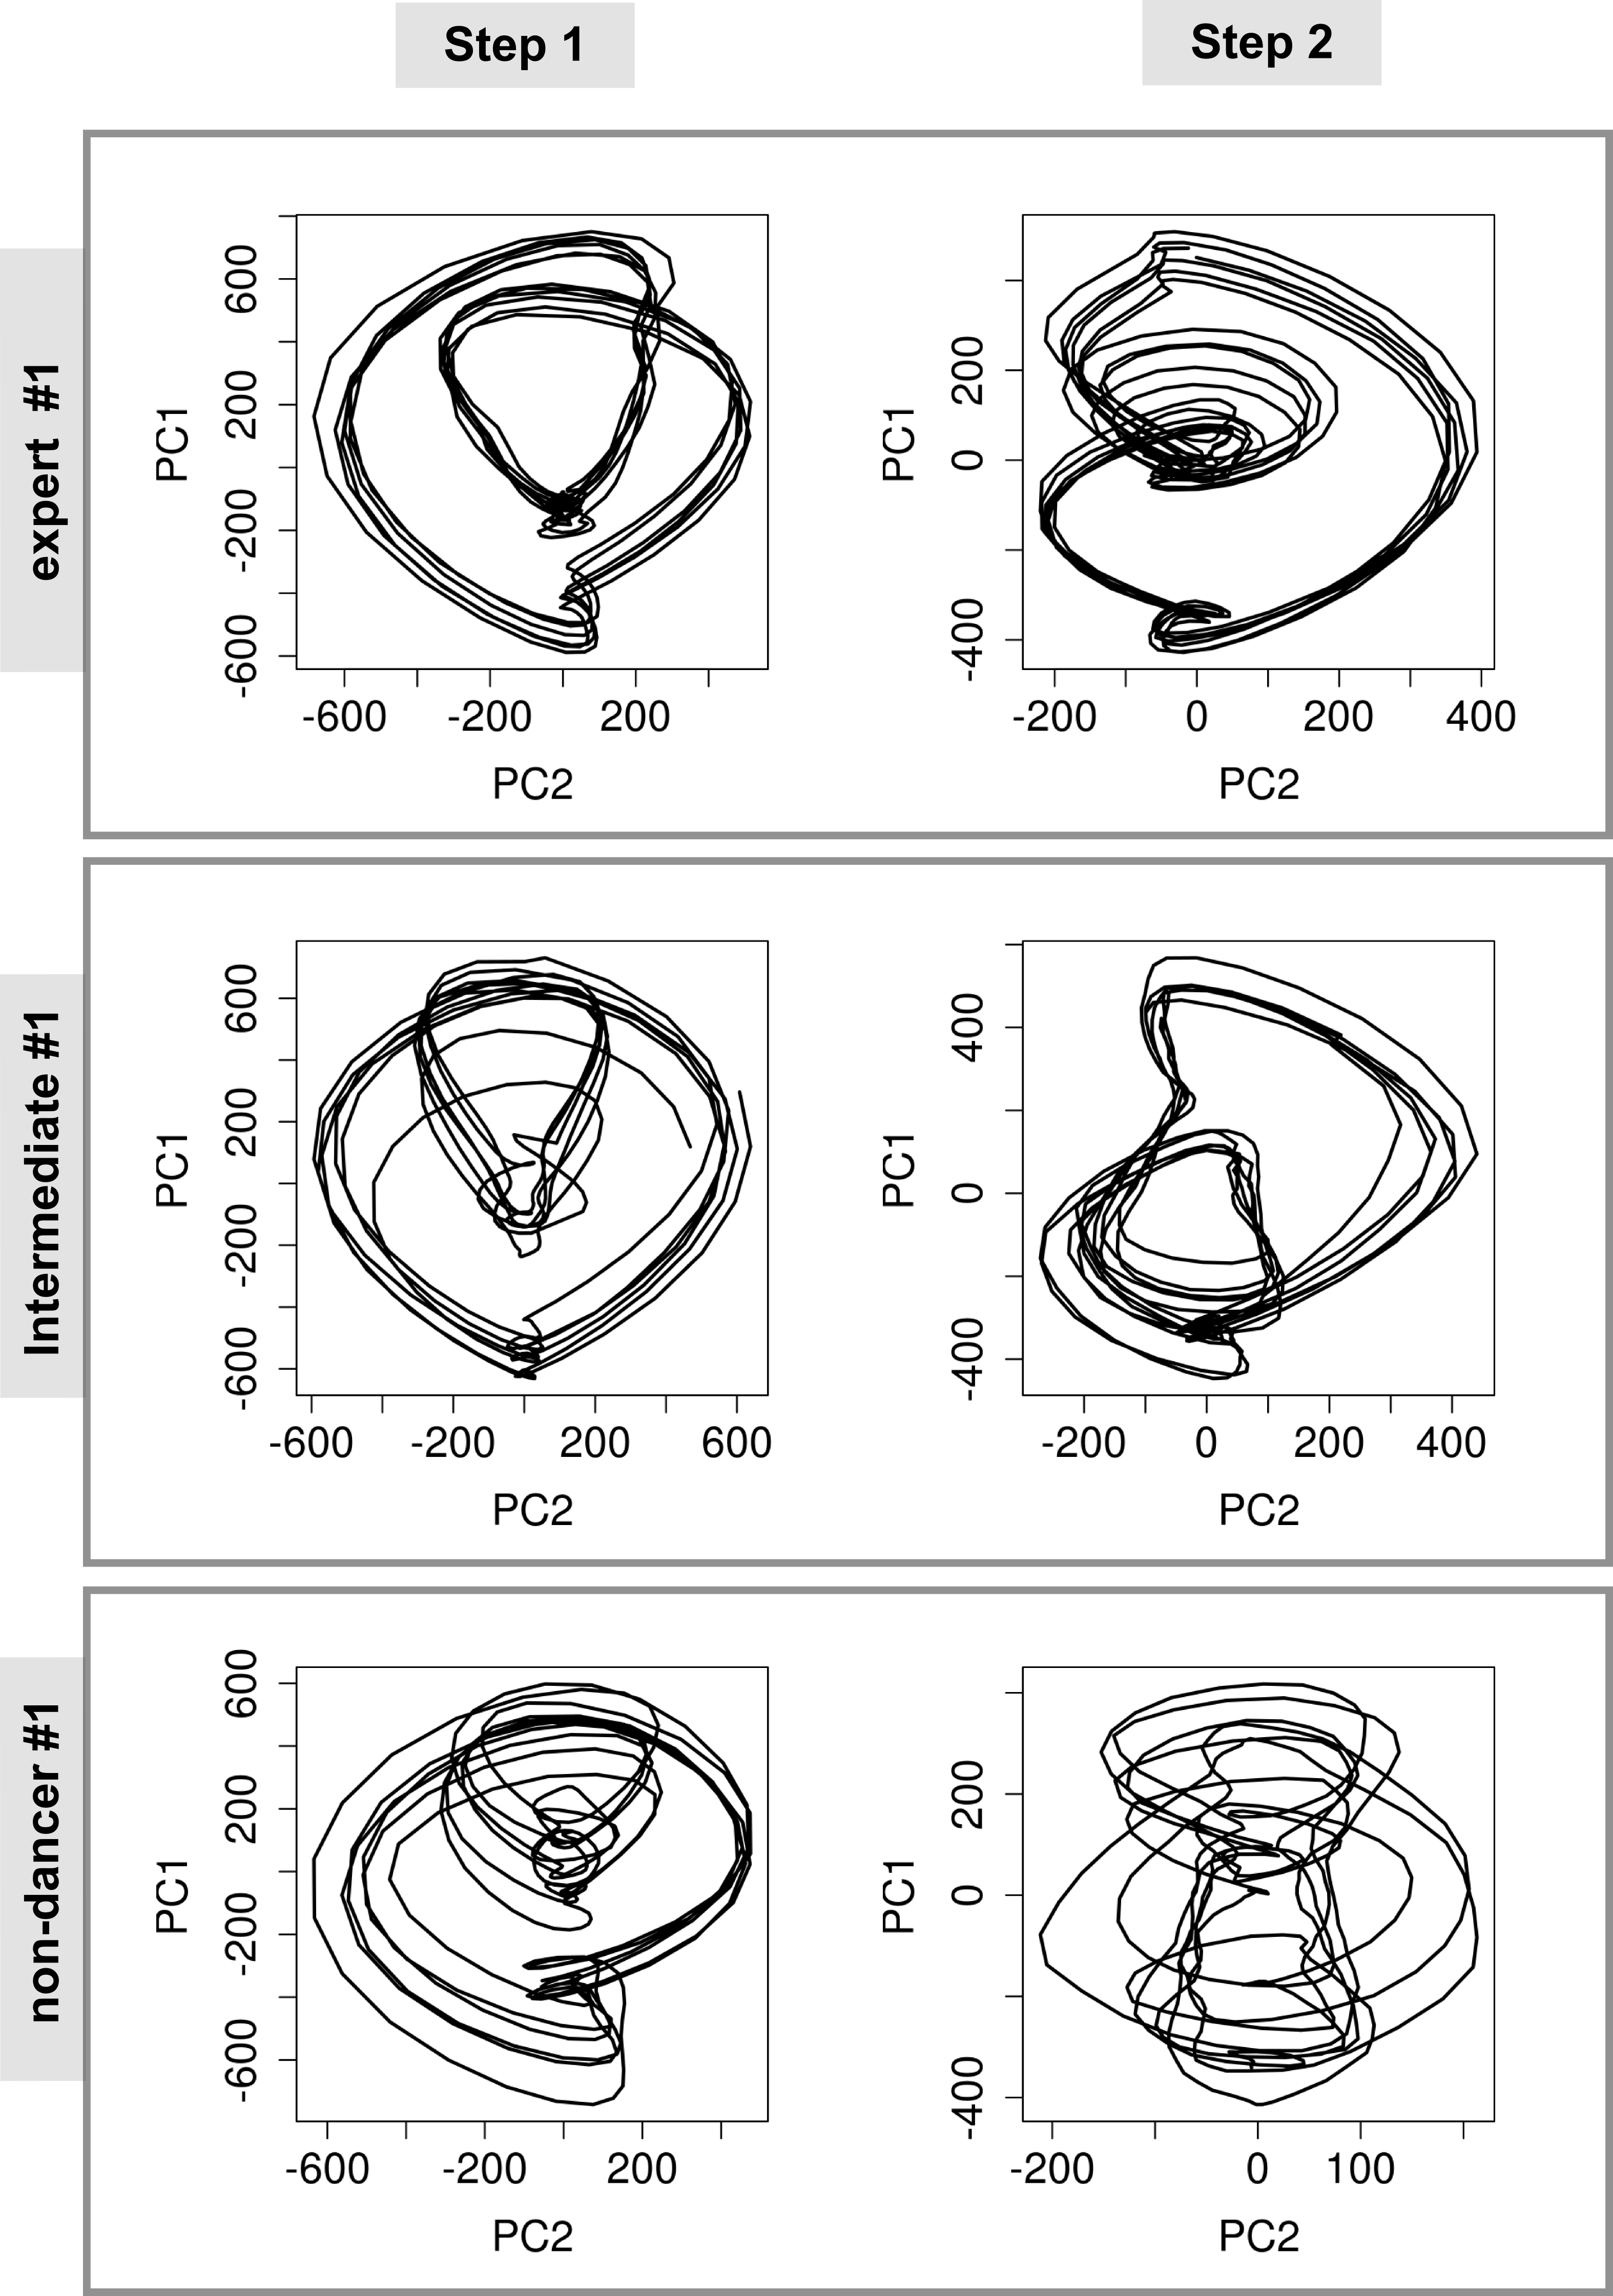
\includegraphics[scale=0.09]{skills} \\
% 
% \end{figure}  
% \end{frame}
% 
% 
% 
% 
% 
% %+++++++++++++++++++++++++++++++++++++++++++++++++++
% \begin{frame}
% \frametitle{Different embedded parameters}
% \vspace{-0.6cm}
% \begin{figure}
% 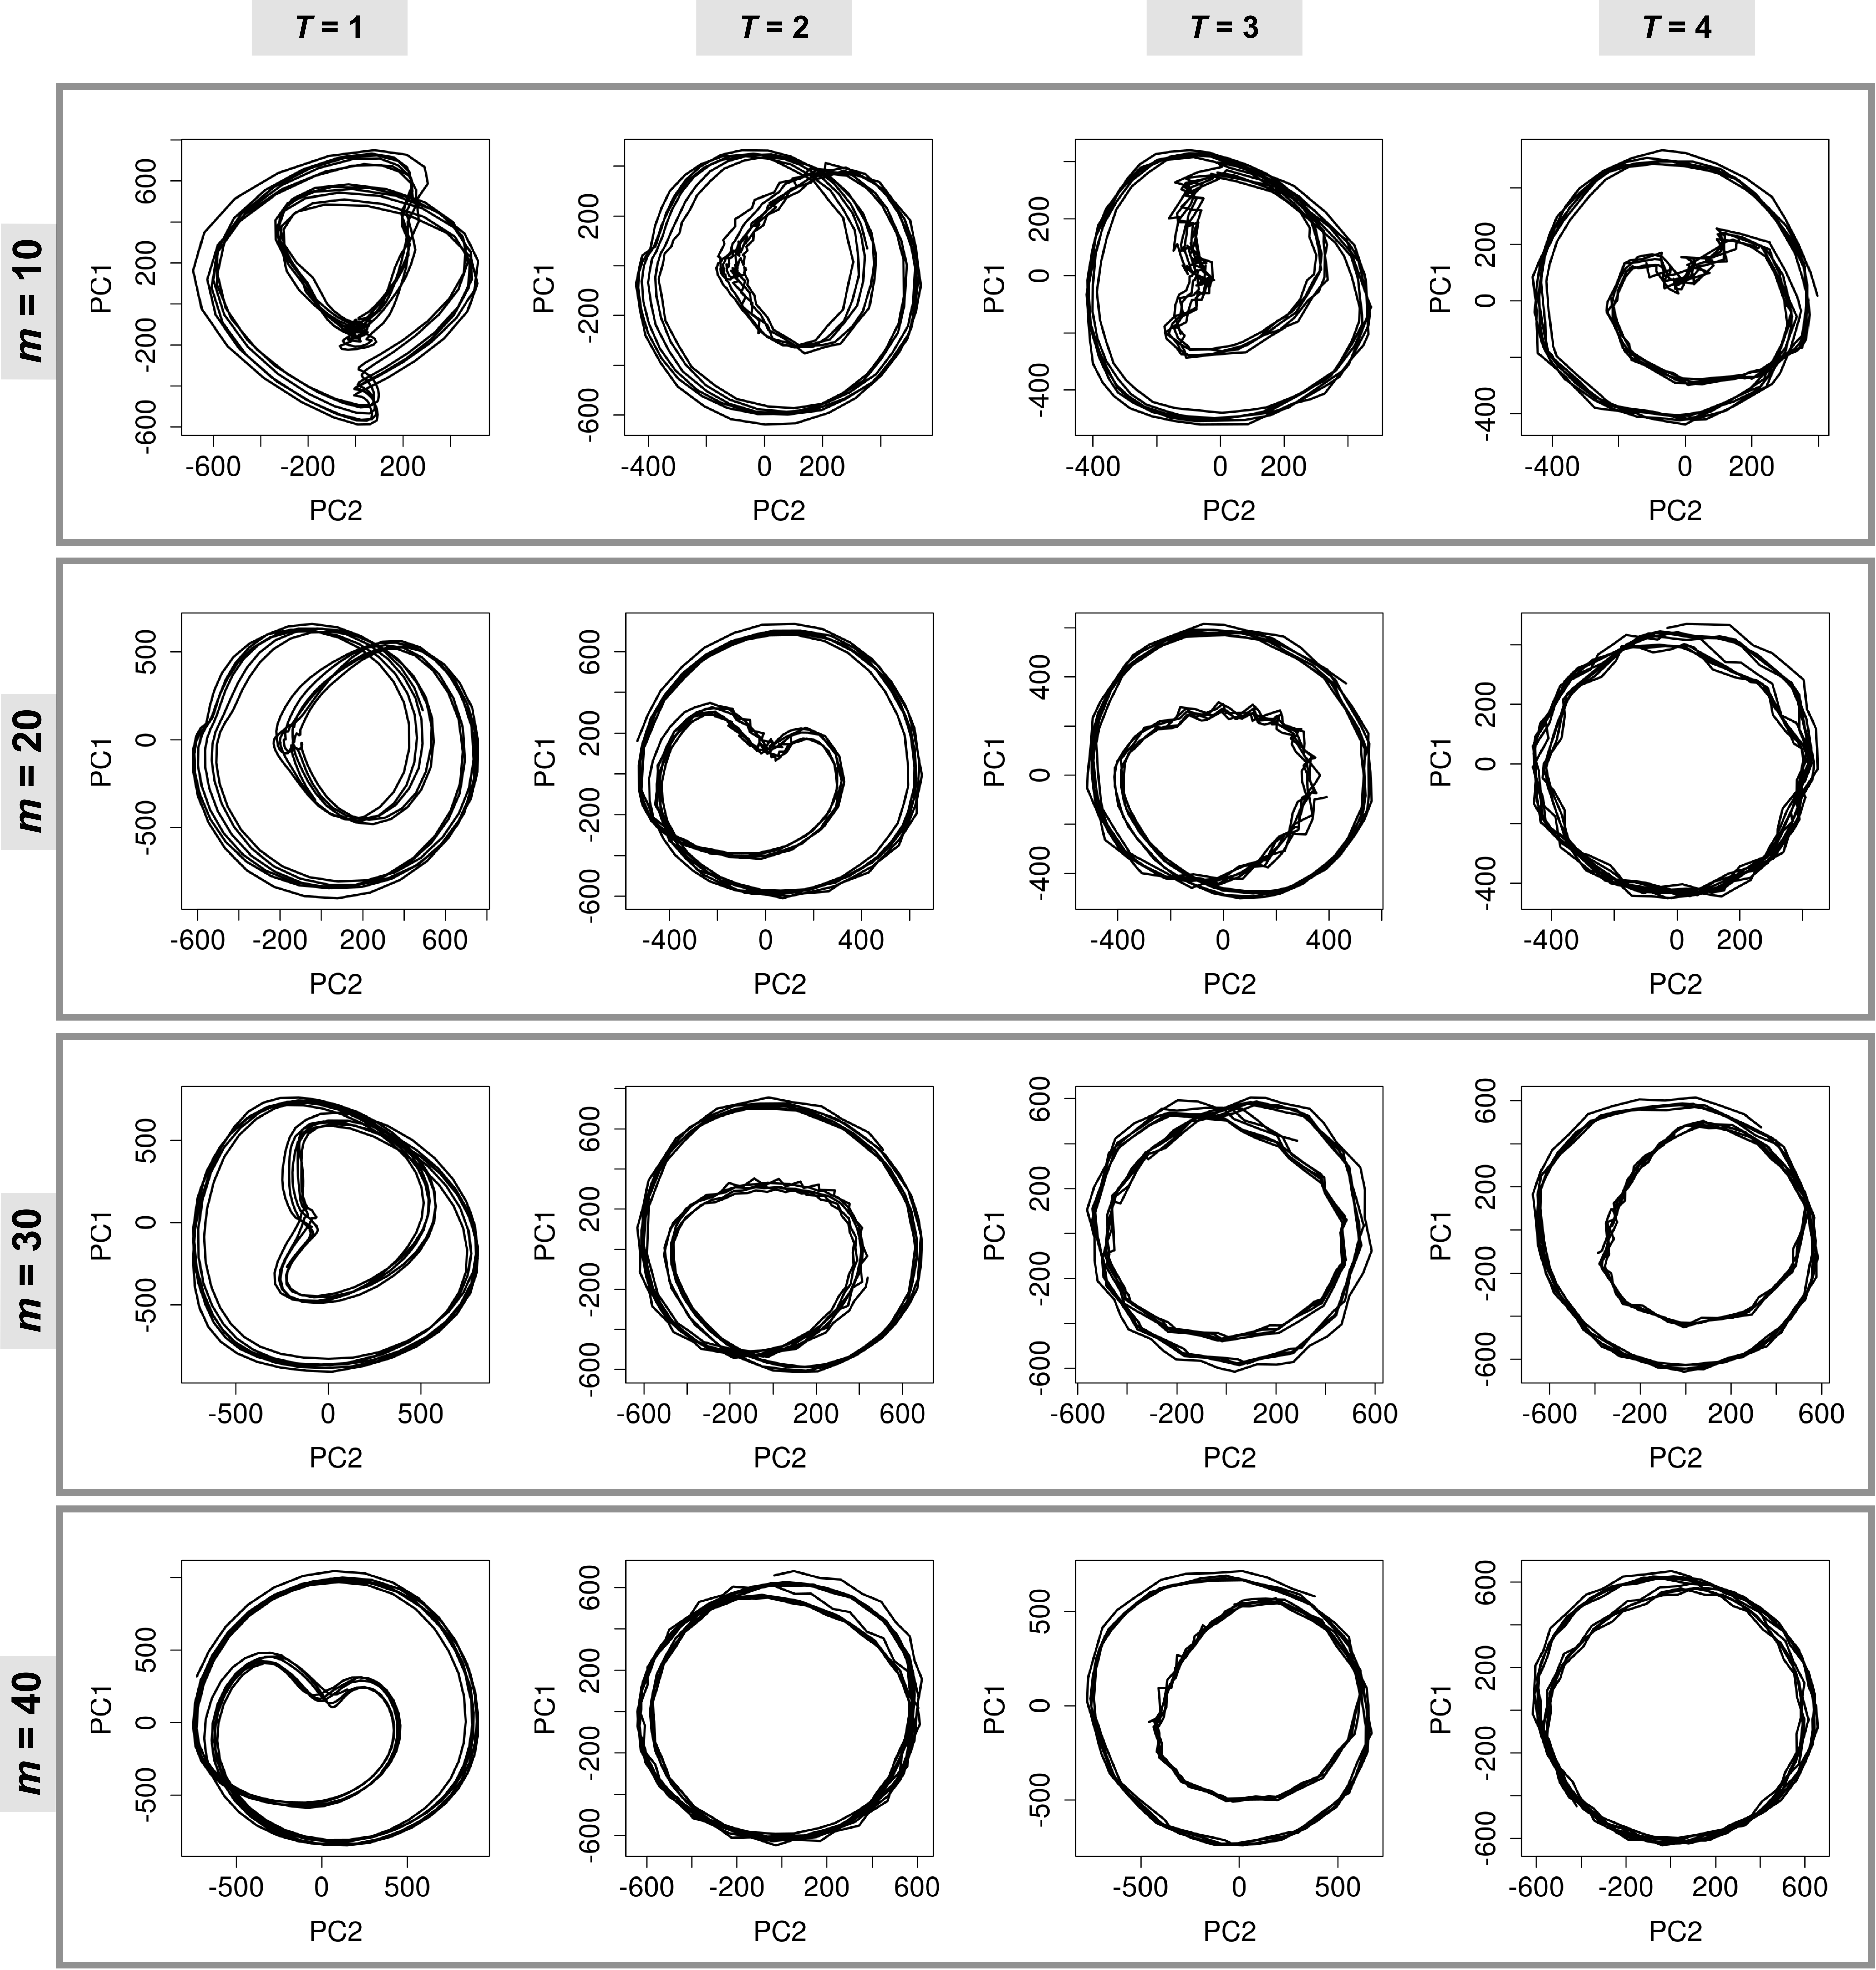
\includegraphics[scale=0.07]{takens} \\
% 
% \end{figure}  
% \end{frame}
% 





% 
% 
% 
% %+++++++++++++++++++++++++++++++++++++++++++++++++++
% \begin{frame}
% \frametitle{RSS for Feet Pattern 2 \\ Participan 0 (Woman)- IMU1 GYR Z }
% \vspace{-0.5cm}
% 
% \begin{figure}
% \centering 
% 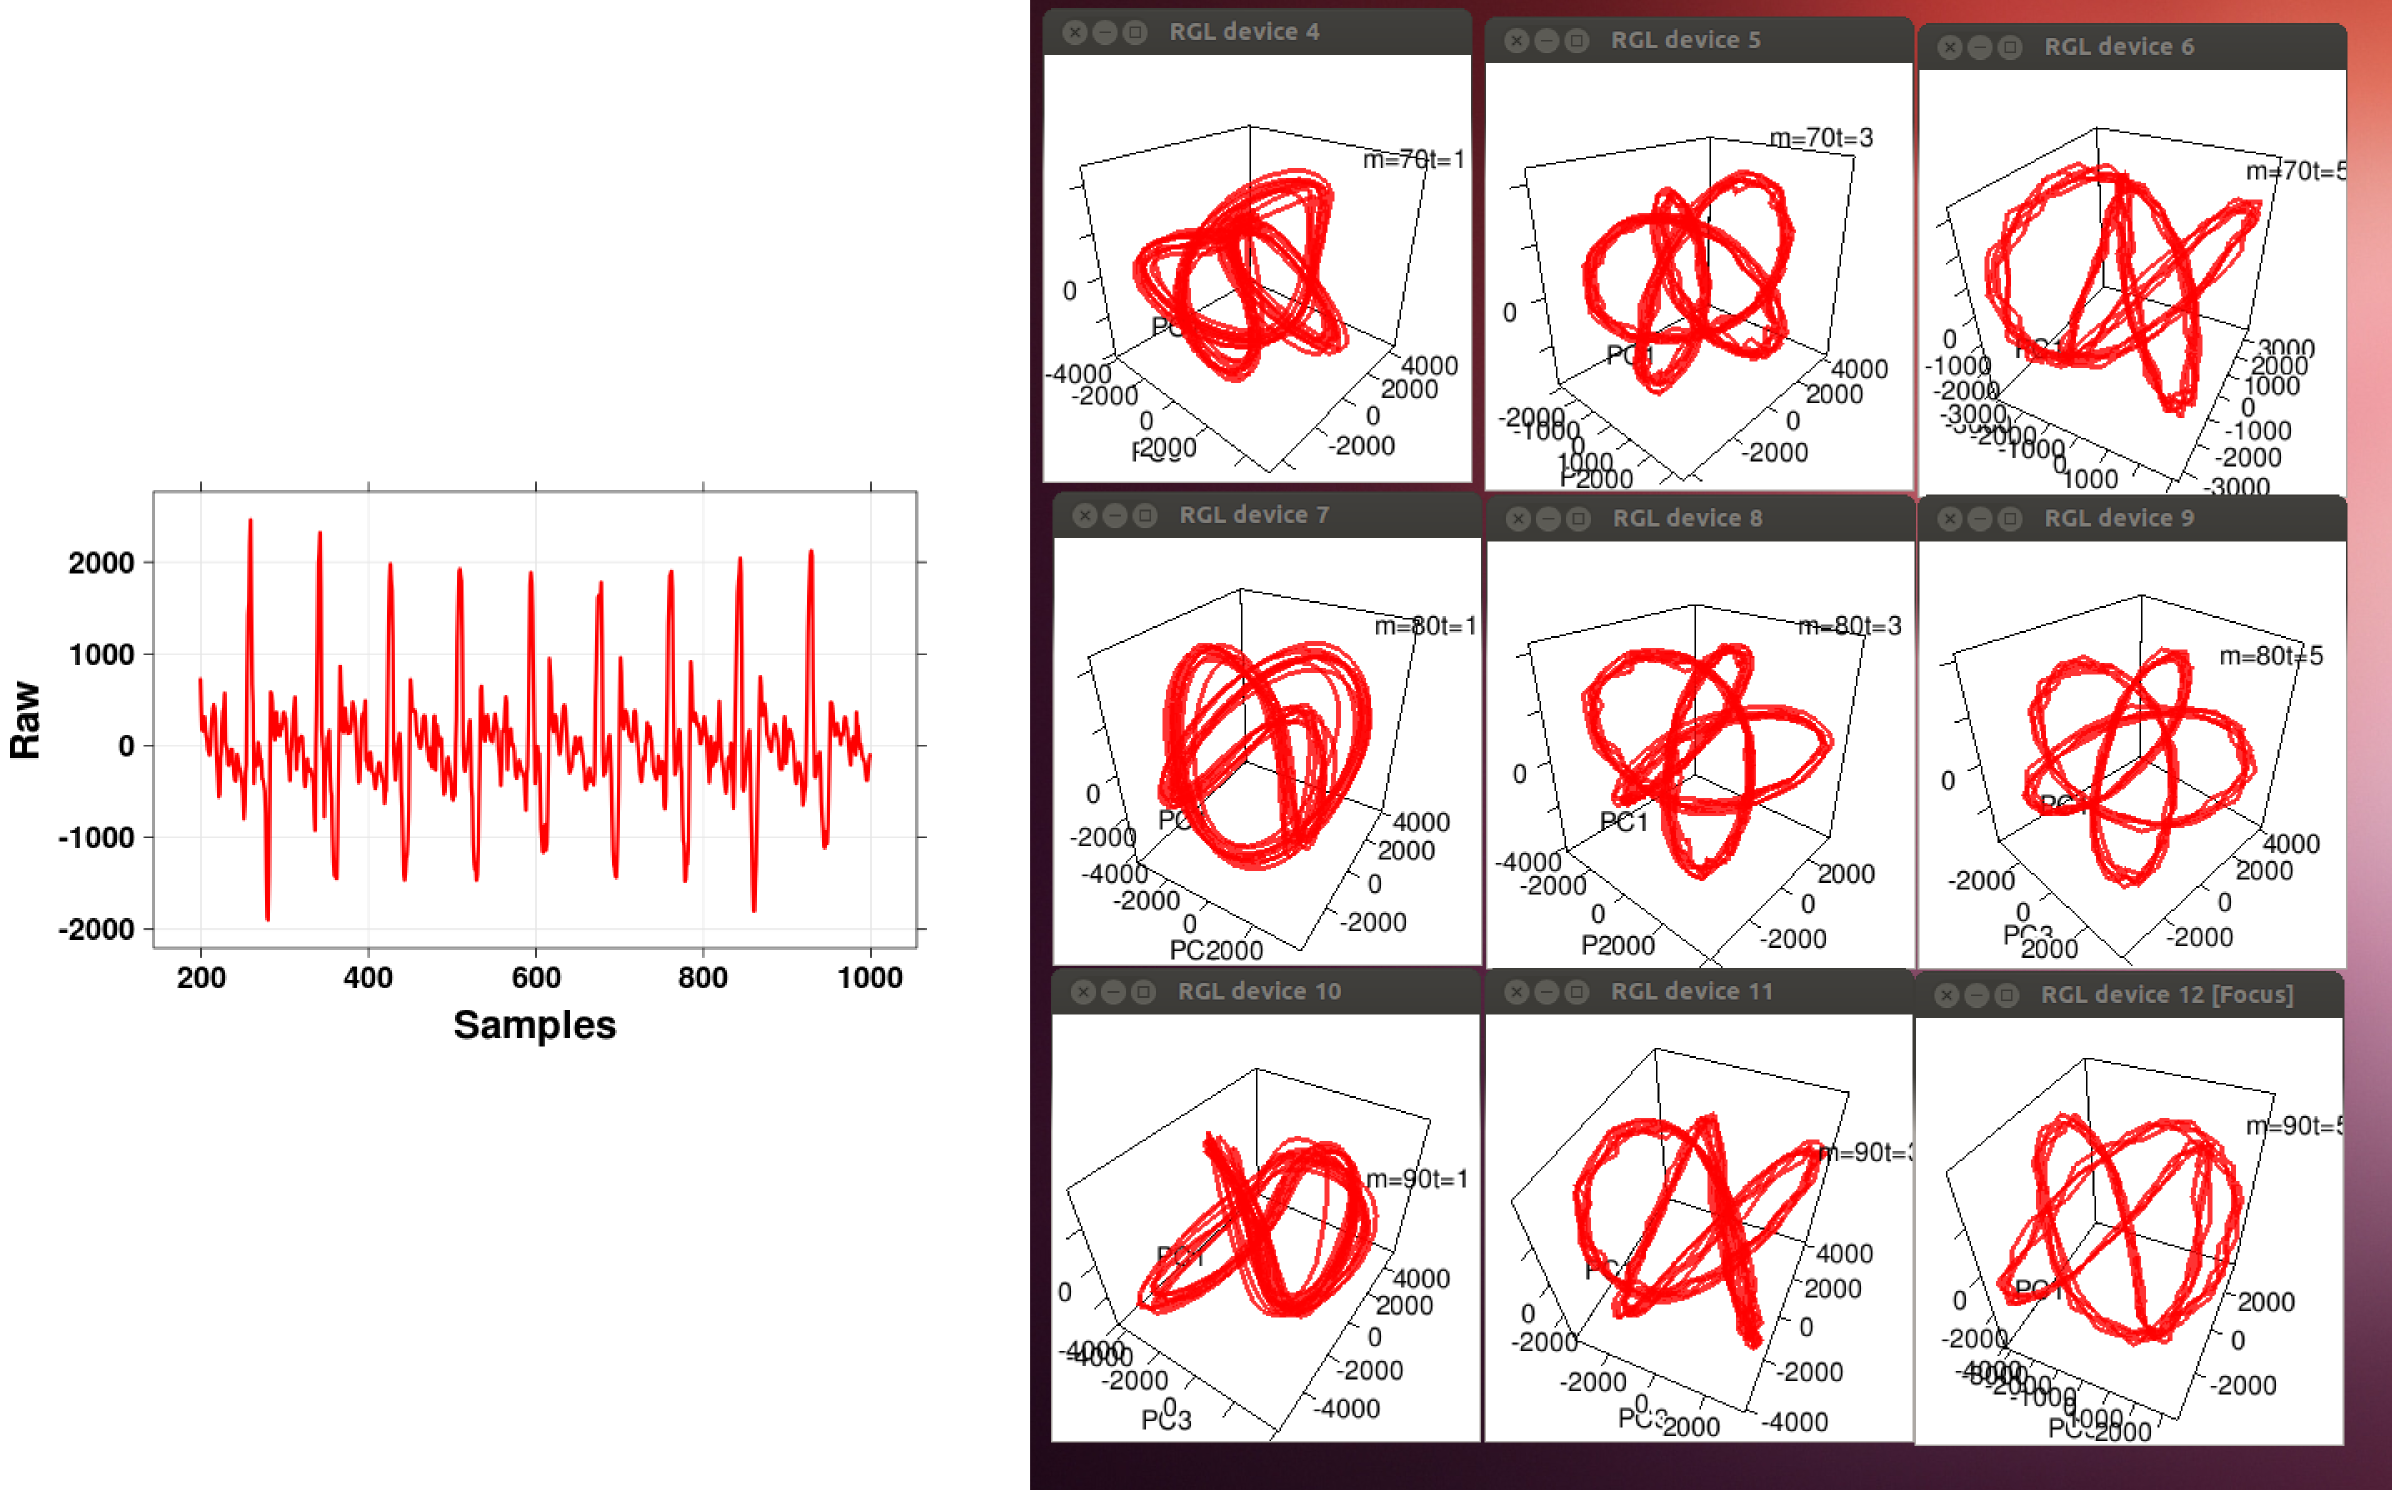
\includegraphics[scale=0.25]{woman0} \\
% \end{figure}
% 
% \end{frame}
% %---------------------------------------------------
% 
% %+++++++++++++++++++++++++++++++++++++++++++++++++++
% \begin{frame}
% \frametitle{RSS for Feet Pattern 2 \\ Participan 1 (Woman) - IMU1 GYR Z }
% \vspace{-0.5cm}
% 
% \begin{figure}
% \centering 
% 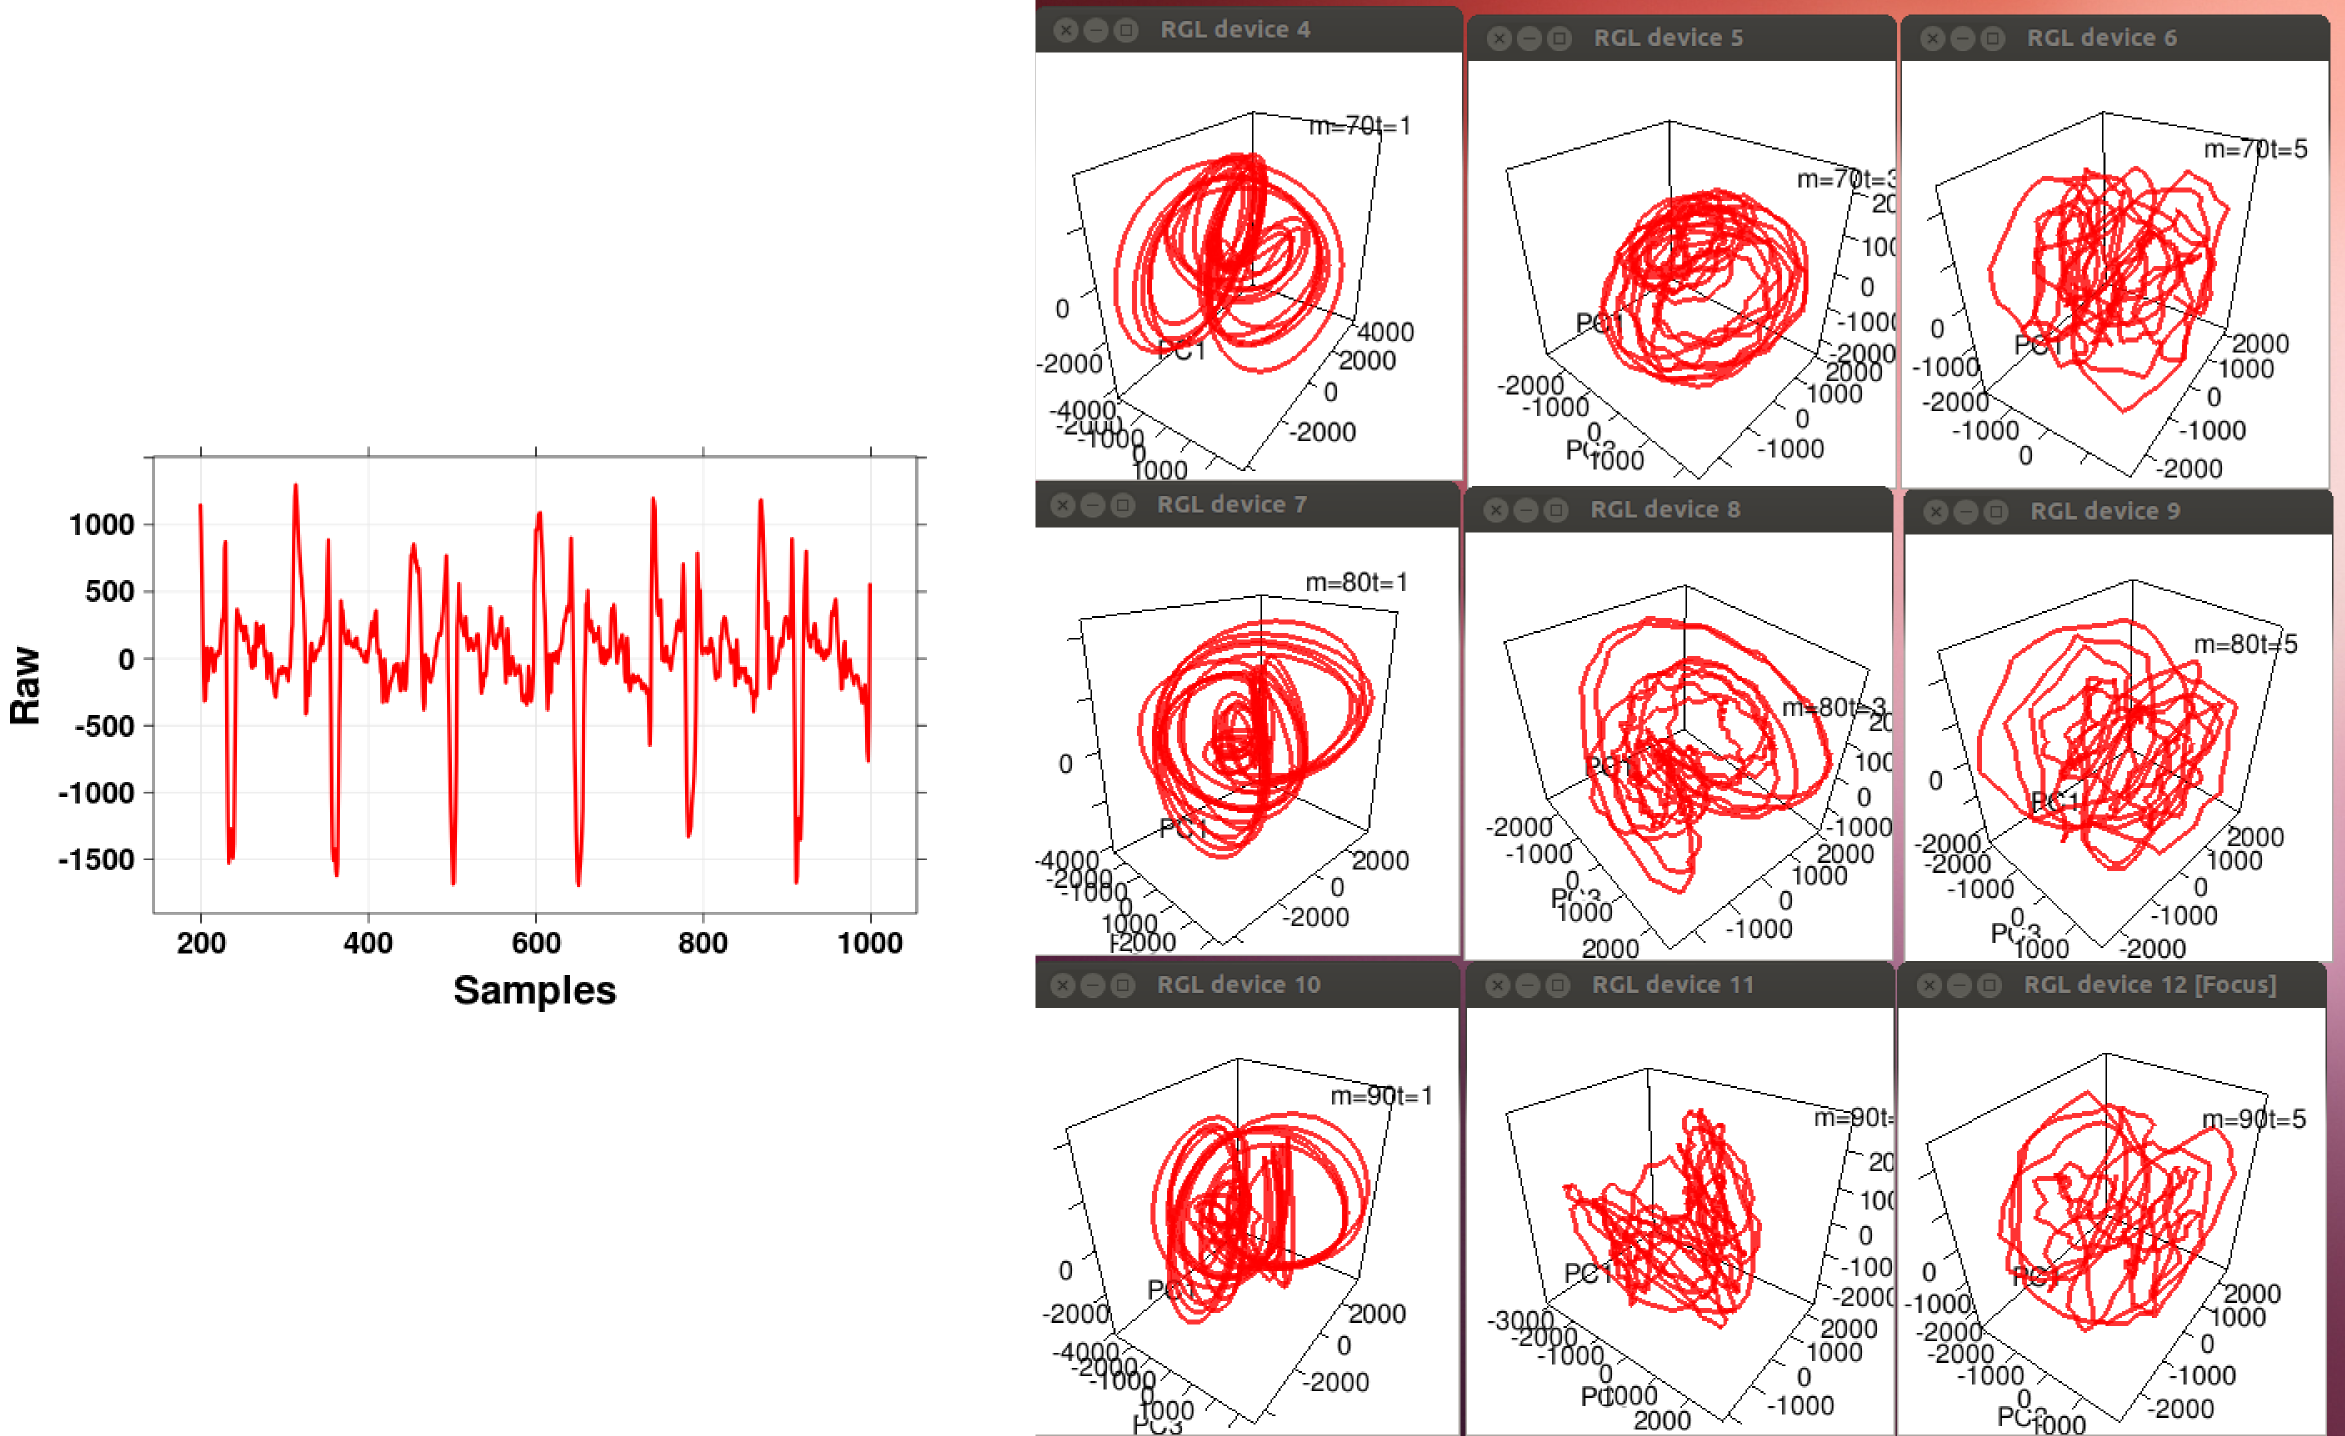
\includegraphics[scale=0.25]{woman1} \\
% \end{figure}
% 
% \end{frame}
% %---------------------------------------------------
% 
% %+++++++++++++++++++++++++++++++++++++++++++++++++++
% \begin{frame}
% \frametitle{RSS for Feet Pattern 2 \\ Participan 2 (Man) - IMU1 GYR Z }
% \vspace{-0.5cm}
% 
% \begin{figure}
% \centering 
% 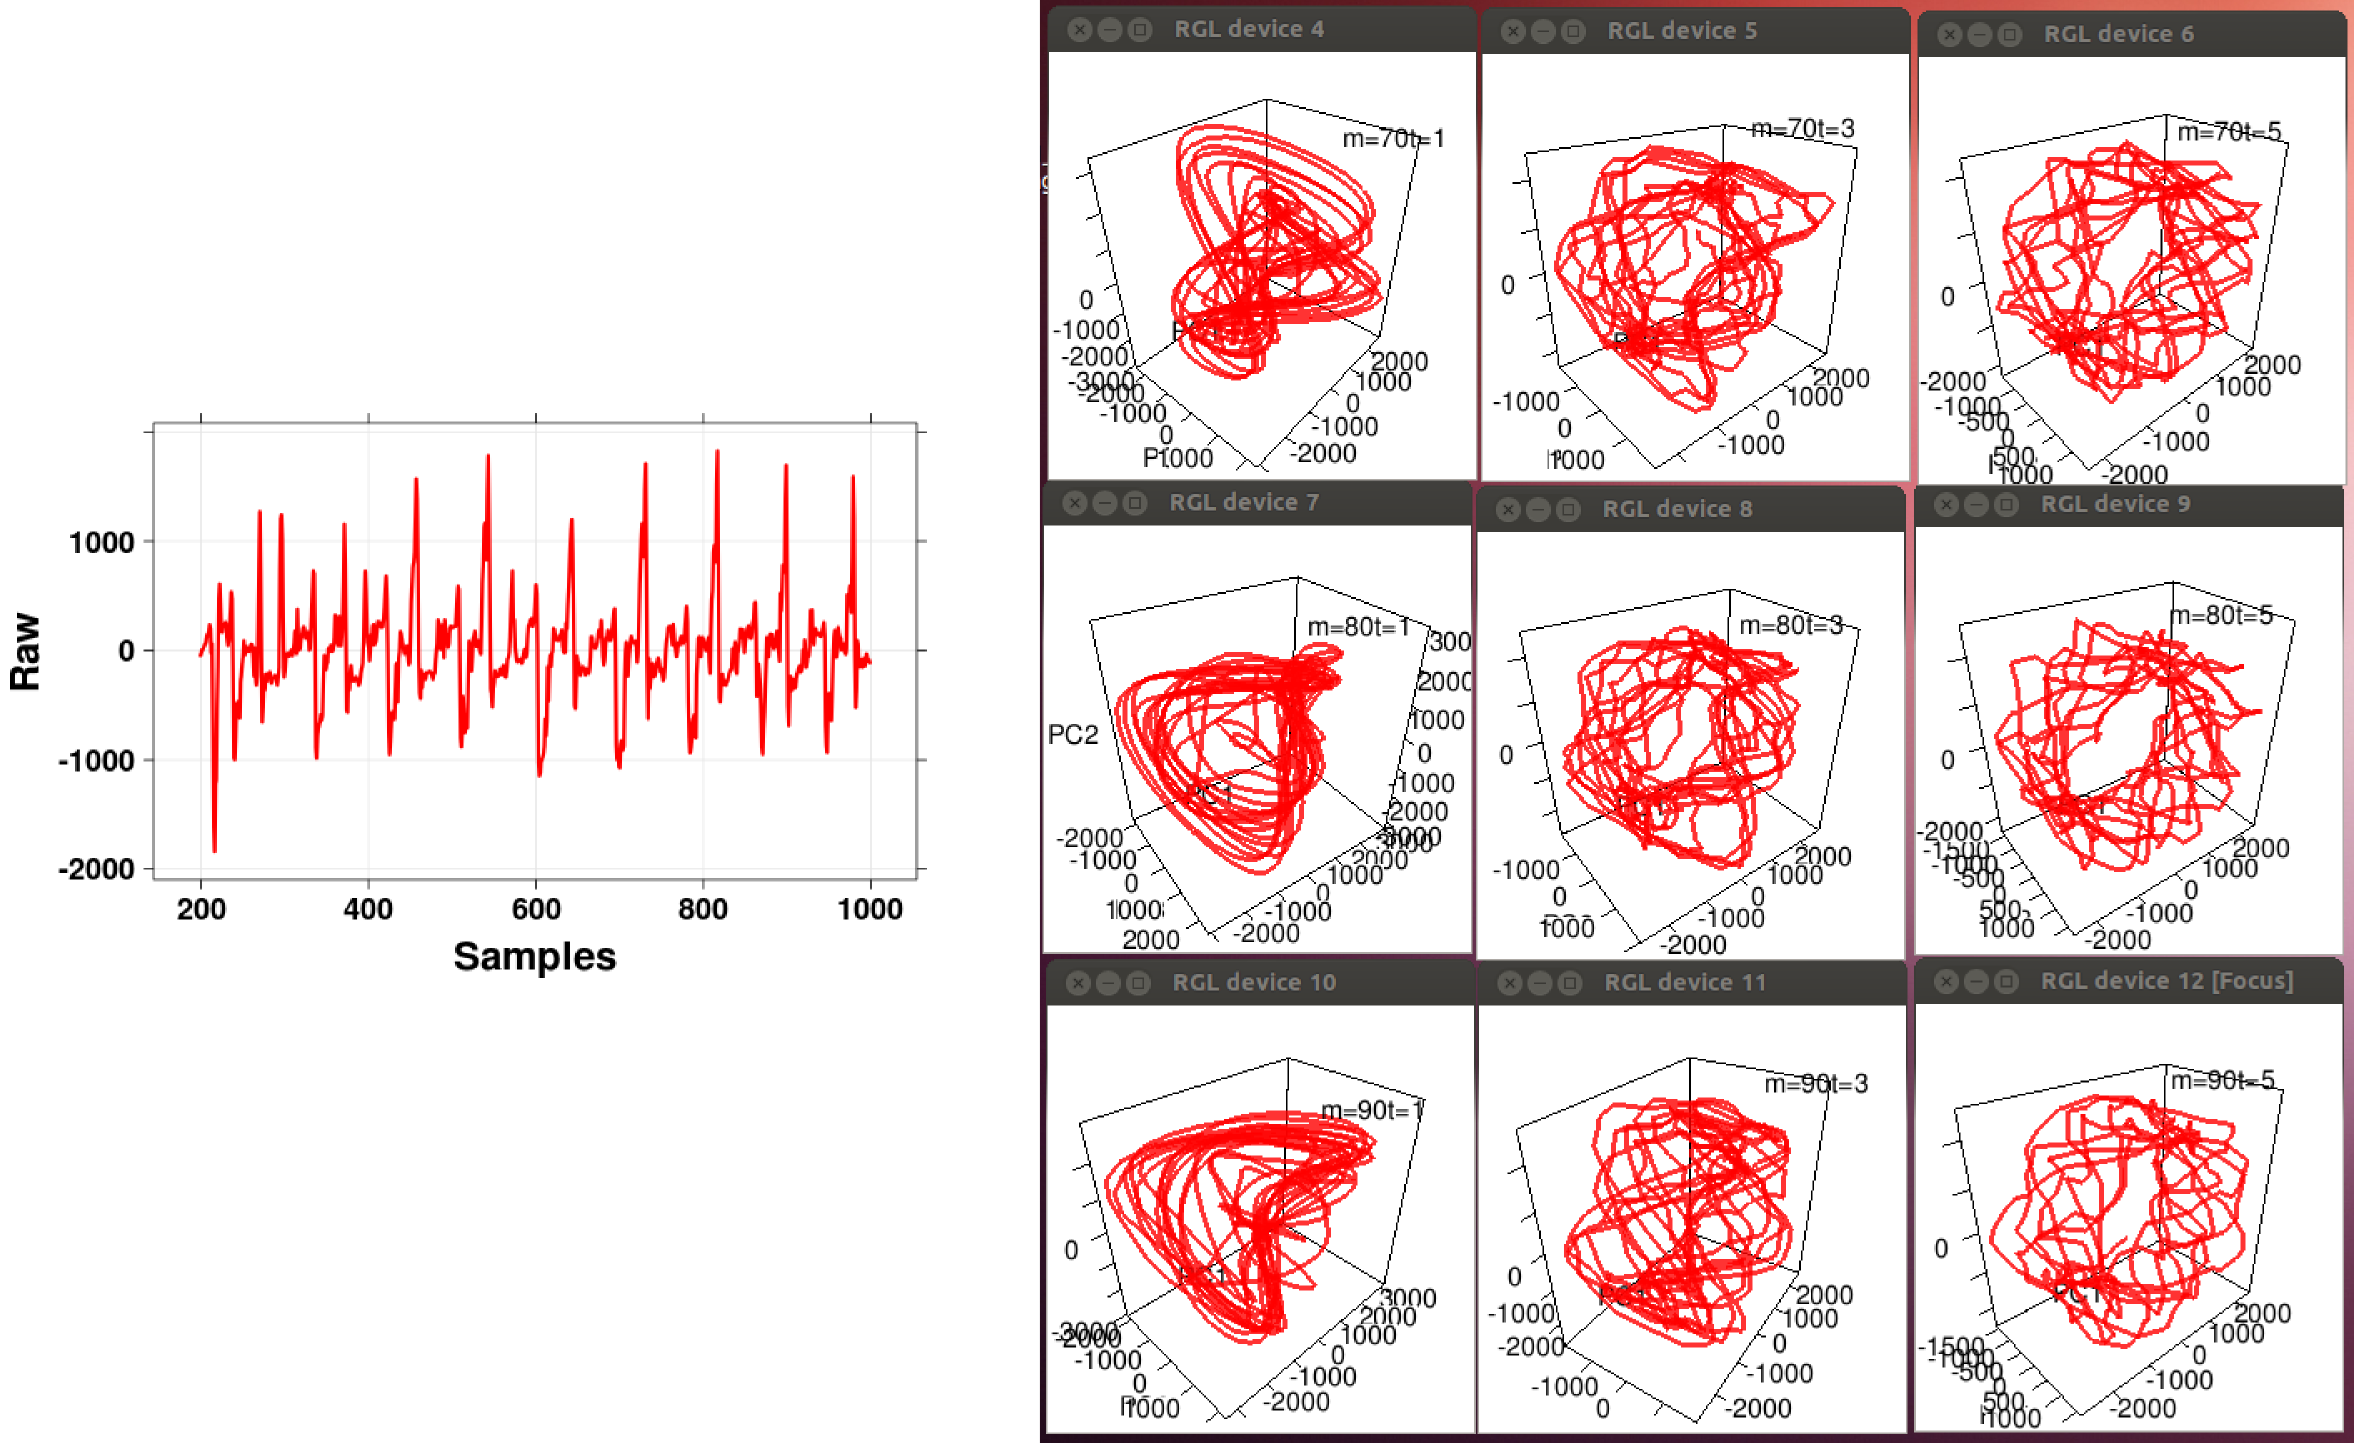
\includegraphics[scale=0.25]{man0} \\
% \end{figure}
% 
% \end{frame}
% %---------------------------------------------------
% 
% %+++++++++++++++++++++++++++++++++++++++++++++++++++
% \begin{frame}
% \frametitle{RSS for Feet Pattern 2 \\ Participan 3 (Man) - IMU1 GYR Z }
% \vspace{-0.5cm}
% 
% \begin{figure}
% \centering 
% 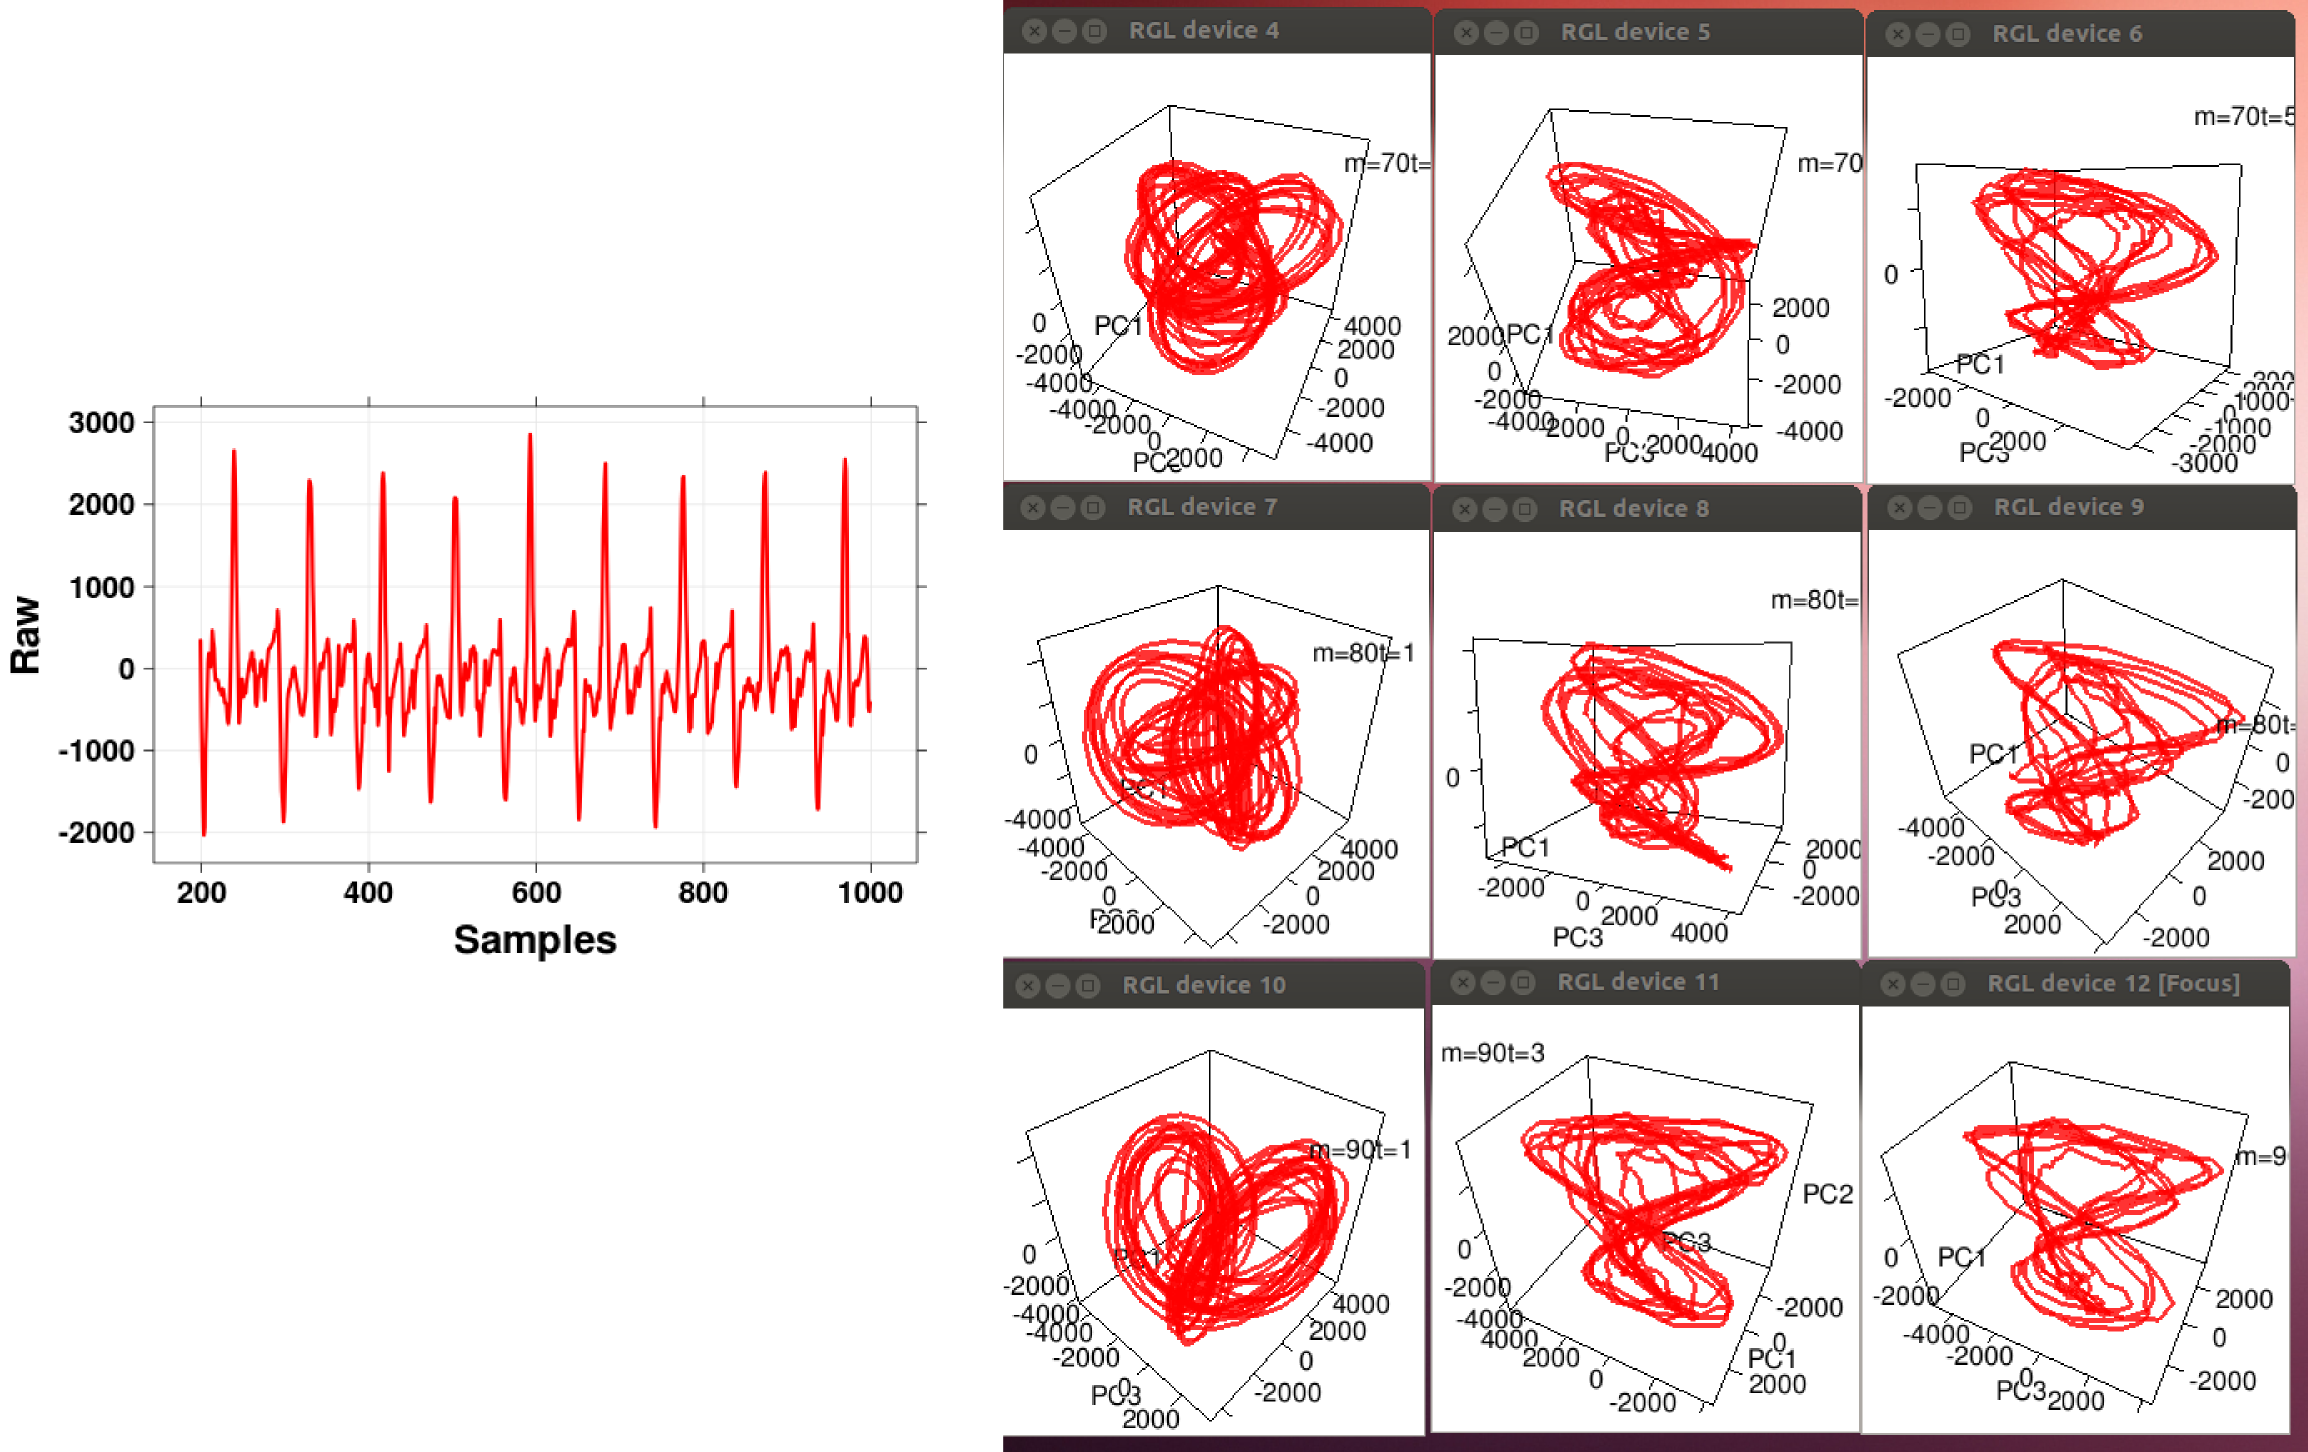
\includegraphics[scale=0.25]{man1} \\
% \end{figure}
% 
% \end{frame}
% %---------------------------------------------------
% 
% %+++++++++++++++++++++++++++++++++++++++++++++++++++
% \begin{frame}
% \frametitle{RSS for Pattern 2 \\ Participan 4 (Man) - IMU1 GYR Z }
% \vspace{-0.5cm}
% 
% \begin{figure}
% \centering 
% 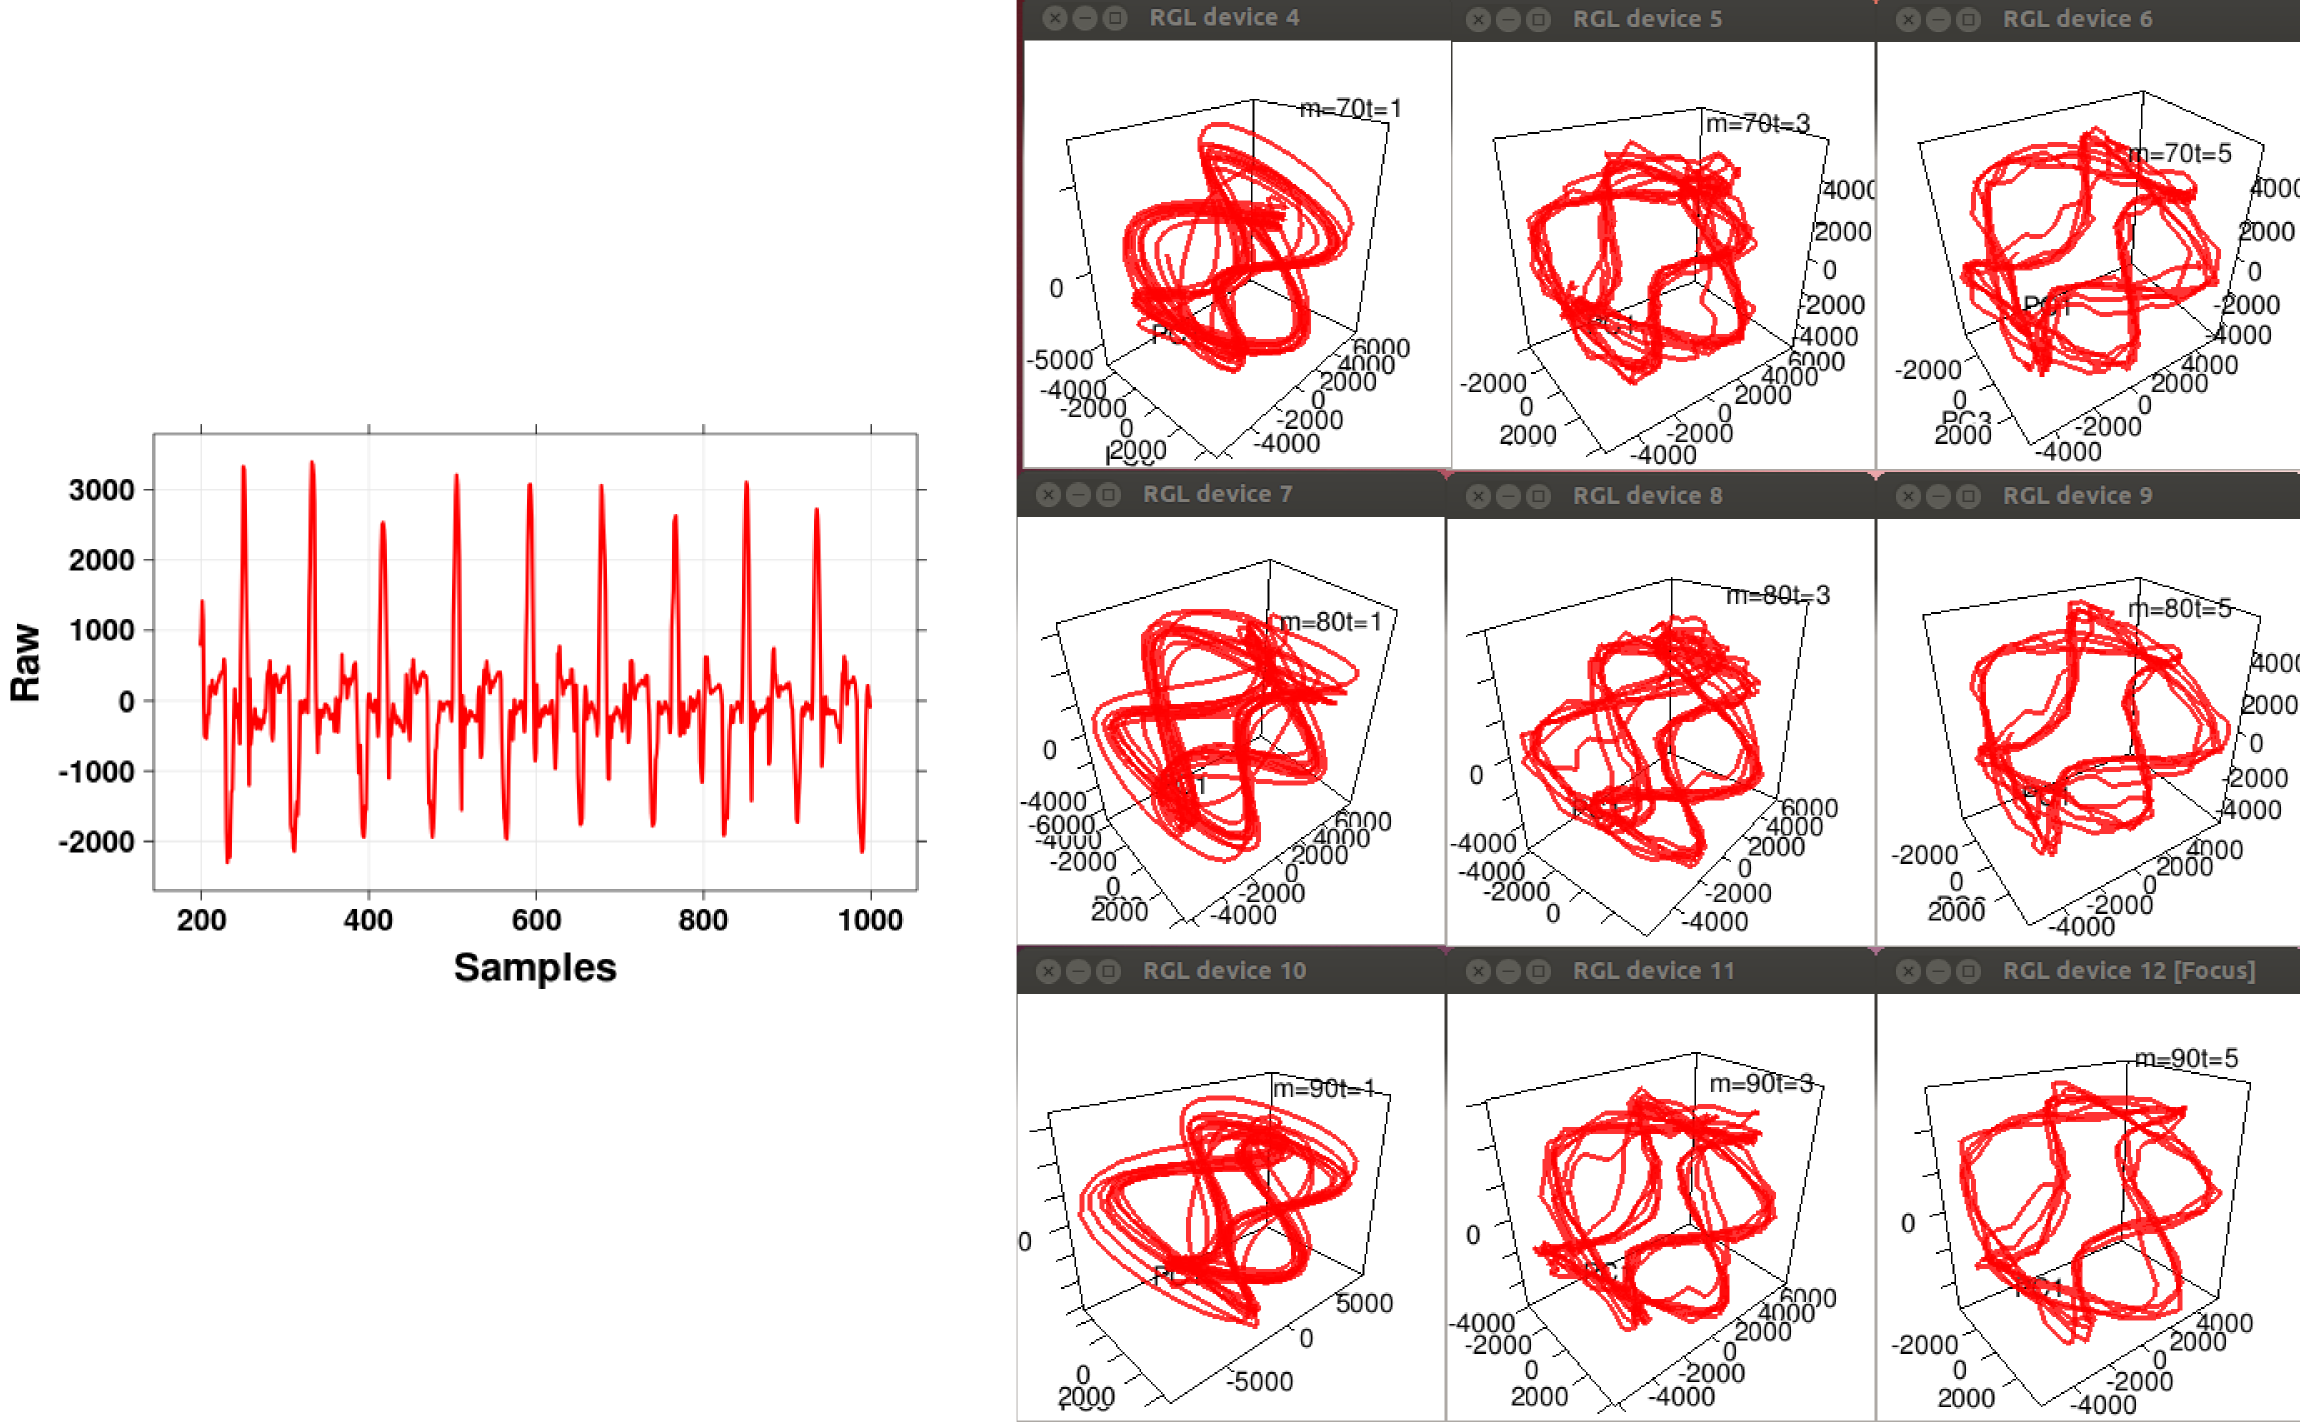
\includegraphics[scale=0.25]{man2} \\
% \end{figure}
% 
% \end{frame}

% %---------------------------------------------------




%+++++++++++++++++++++++++++++++++++++++++++++++++++
%+++++++++++++++++++++++++++++++++++++++++++++++++++
\section{Future Work}

%+++++++++++++++++++++++++++++++++++++++++++++++++++
\begin{frame}
\frametitle{PhD Framework}
\vspace{-0.7cm}

\begin{figure}
\centering 
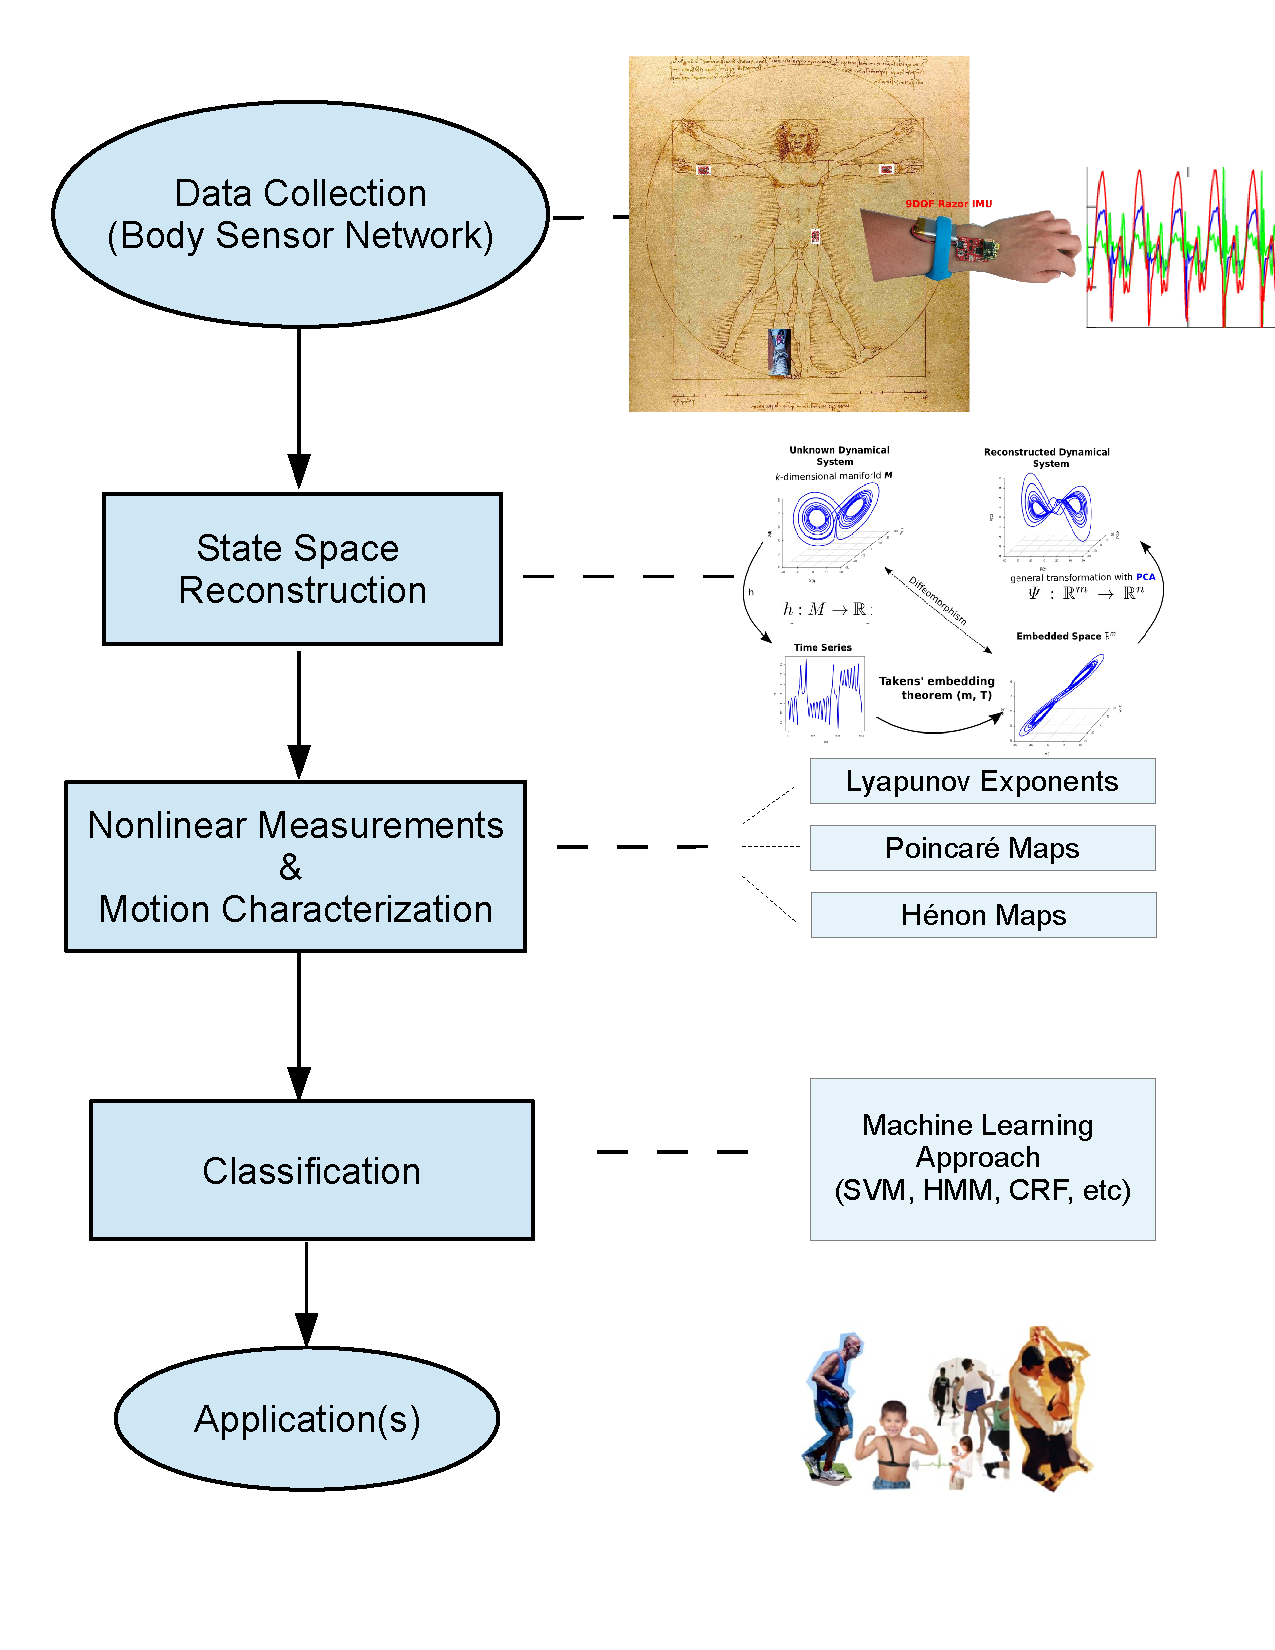
\includegraphics[scale=0.26]{proposedapproach_v1} \\
\end{figure}

\end{frame}
%---------------------------------------------------





%+++++++++++++++++++++++++++++++++++++++++++++++++++
\begin{frame}
\frametitle{}

\vspace{2cm}
\begin{center}
\LARGE{QUESTIONS?} 
\end{center}

\vspace{1cm}

\normalsize 
\textbf{Miguel Perez-Xochicale} \\

E-Mail: {\color{blue} \href{mailto:perez.xochicale@gmail.com}{perez.xochicale@gmail.com} } 

Homepage:
{\color{blue} \href{https://sites.google.com/site/perezxochicale/}{https://sites.google.com/site/perezxochicale/} }
\vspace{1cm}



\includegraphics[scale=.4]{CC4}
\tiny{ 
\textbf{My own pictures are release under CC BY-NC 4.0
{\color{blue} \href{http://creativecommons.org/licenses/by-nc/4.0/}{http://creativecommons.org/licenses/by-nc/4.0/} } \\
Give credits to: Miguel Perez-Xochicale
}
}

\end{frame}
%---------------------------------------------------

% 
% % Creates the cover page.
%  \frame{\titlepage}



\end{document}

